\documentclass[twoside]{book}

% Packages required by doxygen
\usepackage{fixltx2e}
\usepackage{calc}
\usepackage{doxygen}
\usepackage[export]{adjustbox} % also loads graphicx
\usepackage{graphicx}
\usepackage[utf8]{inputenc}
\usepackage{makeidx}
\usepackage{multicol}
\usepackage{multirow}
\PassOptionsToPackage{warn}{textcomp}
\usepackage{textcomp}
\usepackage[nointegrals]{wasysym}
\usepackage[table]{xcolor}

% Font selection
\usepackage[T1]{fontenc}
\usepackage[scaled=.90]{helvet}
\usepackage{courier}
\usepackage{amssymb}
\usepackage{sectsty}
\renewcommand{\familydefault}{\sfdefault}
\allsectionsfont{%
  \fontseries{bc}\selectfont%
  \color{darkgray}%
}
\renewcommand{\DoxyLabelFont}{%
  \fontseries{bc}\selectfont%
  \color{darkgray}%
}
\newcommand{\+}{\discretionary{\mbox{\scriptsize$\hookleftarrow$}}{}{}}

% Page & text layout
\usepackage{geometry}
\geometry{%
  a4paper,%
  top=2.5cm,%
  bottom=2.5cm,%
  left=2.5cm,%
  right=2.5cm%
}
\tolerance=750
\hfuzz=15pt
\hbadness=750
\setlength{\emergencystretch}{15pt}
\setlength{\parindent}{0cm}
\setlength{\parskip}{3ex plus 2ex minus 2ex}
\makeatletter
\renewcommand{\paragraph}{%
  \@startsection{paragraph}{4}{0ex}{-1.0ex}{1.0ex}{%
    \normalfont\normalsize\bfseries\SS@parafont%
  }%
}
\renewcommand{\subparagraph}{%
  \@startsection{subparagraph}{5}{0ex}{-1.0ex}{1.0ex}{%
    \normalfont\normalsize\bfseries\SS@subparafont%
  }%
}
\makeatother

% Headers & footers
\usepackage{fancyhdr}
\pagestyle{fancyplain}
\fancyhead[LE]{\fancyplain{}{\bfseries\thepage}}
\fancyhead[CE]{\fancyplain{}{}}
\fancyhead[RE]{\fancyplain{}{\bfseries\leftmark}}
\fancyhead[LO]{\fancyplain{}{\bfseries\rightmark}}
\fancyhead[CO]{\fancyplain{}{}}
\fancyhead[RO]{\fancyplain{}{\bfseries\thepage}}
\fancyfoot[LE]{\fancyplain{}{}}
\fancyfoot[CE]{\fancyplain{}{}}
\fancyfoot[RE]{\fancyplain{}{\bfseries\scriptsize Generated by Doxygen }}
\fancyfoot[LO]{\fancyplain{}{\bfseries\scriptsize Generated by Doxygen }}
\fancyfoot[CO]{\fancyplain{}{}}
\fancyfoot[RO]{\fancyplain{}{}}
\renewcommand{\footrulewidth}{0.4pt}
\renewcommand{\chaptermark}[1]{%
  \markboth{#1}{}%
}
\renewcommand{\sectionmark}[1]{%
  \markright{\thesection\ #1}%
}

% Indices & bibliography
\usepackage{natbib}
\usepackage[titles]{tocloft}
\setcounter{tocdepth}{3}
\setcounter{secnumdepth}{5}
\makeindex

% Hyperlinks (required, but should be loaded last)
\usepackage{ifpdf}
\ifpdf
  \usepackage[pdftex,pagebackref=true]{hyperref}
\else
  \usepackage[ps2pdf,pagebackref=true]{hyperref}
\fi
\hypersetup{%
  colorlinks=true,%
  linkcolor=blue,%
  citecolor=blue,%
  unicode%
}

% Custom commands
\newcommand{\clearemptydoublepage}{%
  \newpage{\pagestyle{empty}\cleardoublepage}%
}

\usepackage{caption}
\captionsetup{labelsep=space,justification=centering,font={bf},singlelinecheck=off,skip=4pt,position=top}

%===== C O N T E N T S =====

\begin{document}

% Titlepage & ToC
\hypersetup{pageanchor=false,
             bookmarksnumbered=true,
             pdfencoding=unicode
            }
\pagenumbering{alph}
\begin{titlepage}
\vspace*{7cm}
\begin{center}%
{\Large Pink\+\_\+server\+\_\+doxygen }\\
\vspace*{1cm}
{\large Generated by Doxygen 1.8.13}\\
\end{center}
\end{titlepage}
\clearemptydoublepage
\pagenumbering{roman}
\tableofcontents
\clearemptydoublepage
\pagenumbering{arabic}
\hypersetup{pageanchor=true}

%--- Begin generated contents ---
\chapter{架构与模块}
\label{md_knowledge_architecture}
\Hypertarget{md_knowledge_architecture}
{\bfseries Preview\+: 基于 Reactor 的半同步/半异步并发模式 + 同步 epoll (ET) 事件循环 + 多线程 (线程池)} 



\paragraph*{整体结构与详细工作流}

 



\subsubsection*{各大模块}

\paragraph*{1. Epoll 事件循环}

{\bfseries \hyperlink{pink__epoll_8h}{pink\+\_\+epoll.\+h}$\vert$cpp + \hyperlink{pink__epoll__tool_8h}{tools/pink\+\_\+epoll\+\_\+tool.\+h}$\vert$cpp}

在整体架构中,epoll 属于同步的部分,由主线程同步运行。


\begin{DoxyItemize}
\item {\bfseries 结构}
\end{DoxyItemize}
\begin{DoxyEnumerate}
\item 采用 ET 模式。(同时实现了 LT 模式。)
\item 注册的事件类型\+: (1)新连接请求到来(2)连接socket上读就绪(3)连接socket上写就绪
\item 只负责接受连接,分发读取/写出任务,以及定时器超时任务。
\item 定期处理超时事件\+: 目前每5秒。
\end{DoxyEnumerate}

\paragraph*{2. 连接池}

{\bfseries \hyperlink{pink__conn__pool_8h}{pink\+\_\+conn\+\_\+pool.\+h}}

为了节约连接体申请内存的时间开销,采用连接池进行优化。


\begin{DoxyItemize}
\item {\bfseries 结构}
\end{DoxyItemize}
\begin{DoxyEnumerate}
\item 通过预先分配 pre\+\_\+conn\+\_\+number 个连接体来构建连接池。
\item 核心\+: list$<$\+T$\ast$$>$ conn\+\_\+lst 连接体指针链表。
\item 每次从表头获取连接体指针(即原先的 new),每次归还连接体指针到表尾(即原先的 delete)。
\end{DoxyEnumerate}
\begin{DoxyItemize}
\item {\bfseries 题外话}
\end{DoxyItemize}
\begin{DoxyEnumerate}
\item 一开始实现连接池时,打算用连接体数组,并搭配最小堆来存放连接体下标,每次分配最小可用下标的连接体 O(log\+K)。分配连接的时间效率肯定不如现在的链表形式 O(1)。但是最小堆的内存局部性更强。
\item 实际上直接用连接体数组,并用 fd 来直接做下标也是可行的。但总觉得不够优雅。
\end{DoxyEnumerate}

\paragraph*{3. 时间堆}

{\bfseries \hyperlink{pink__conn__timer_8h}{pink\+\_\+conn\+\_\+timer.\+h} + \hyperlink{pink__epoll_8h}{pink\+\_\+epoll.\+h}$\vert$cpp}


\begin{DoxyItemize}
\item {\bfseries 结构}
\end{DoxyItemize}
\begin{DoxyEnumerate}
\item 采用自实现的最小堆,存放定时器的指针。
\item 每次处理时不断从顶部取出定时器,并判断是否超时。
\item 删除定时器采用懒惰删除,给定时器打上 cancled 标签。
\end{DoxyEnumerate}

\paragraph*{4. 线程池}

{\bfseries \hyperlink{pink__thread__pool_8h}{pink\+\_\+thread\+\_\+pool.\+h}}


\begin{DoxyItemize}
\item {\bfseries 结构}
\end{DoxyItemize}
\begin{DoxyEnumerate}
\item {\bfseries 半同步/半反应堆模式$\ast$$\ast$,工作队列($\ast$$\ast$同步})负责任务获取与分发,工作线程({\bfseries 异步})负责处理任务。
\item 工作队列\+: list$<$pair$<$\+T$\ast$, int$>$$>$,每个任务包含结构体和一个标签 flag,用于标记 R\+E\+A\+D/\+W\+R\+I\+TE 任务。
\item 工作线程\+: shared\+\_\+ptr$<$pthread\+\_\+t$>$ threads,线程线程标识符数组,预分配大小。
\end{DoxyEnumerate}
\begin{DoxyItemize}
\item {\bfseries 优点}
\end{DoxyItemize}
\begin{DoxyEnumerate}
\item 以空间换取时间效率。
\item 线程池适用于高并发多线程,但每个线程运行时间较短的情况。
\item 通用性高,比较 general,采用模板元编程。
\end{DoxyEnumerate}
\begin{DoxyItemize}
\item {\bfseries 限制}
\end{DoxyItemize}
\begin{DoxyEnumerate}
\item 要求客户请求都是无状态的,同一个连接上的不同请求可能由不同的线程处理。
\item 容易产生惊群效应,需要特殊处理。
\end{DoxyEnumerate}

\paragraph*{5. 工作线程}


\begin{DoxyEnumerate}
\item 工作线程取出读取/写出任务后,回调 H\+T\+TP 连接类的 process() 函数。
\item 回调一次 process() 函数负责\+:
\end{DoxyEnumerate}

(1)从内核缓冲区读取数据到用户缓冲区\+: 非阻塞 read,(遇到 E\+A\+G\+A\+IN 则返回)

(2)处理 H\+T\+TP 请求报文

(3)构建 H\+T\+TP 响应报文

(4)把响应报文写入到内核缓冲区\+: 非阻塞 write,(遇到 E\+A\+G\+A\+IN 则返回)


\begin{DoxyEnumerate}
\item {\bfseries 如果能一次性处理完则不再通知 epoll} 
\end{DoxyEnumerate}
\chapter{基础知识}
\label{md_knowledge_basic}
\Hypertarget{md_knowledge_basic}




\paragraph*{服务器并发模式分析}

{\bfseries 1. 单进程多线程模式}

通过在单进程内创建线程池,使工作线程异步并行地为客户的请求服务。

{\bfseries 优点:}

(1)工作线程之间数据共享方便(全局、静态变量)。

(2)线程的上下文切换开销较小(不切换地址空间,不刷新 T\+L\+B,只修改部分 C\+PU 寄存器),善于处理高并发。

(3)线程创建速度较快。

{\bfseries 缺点:}

(1)一个线程挂了,其他线程也就挂了。(虽然能写守护进程来重启,但是会有宕机期。)

(2)编程时需要考虑资源的同步问题,稍显复杂。

{\bfseries 2. 多进程单线程模式}

{\bfseries 优点:}

(1)一个进程崩溃可以被 master 重启,并不会使整个服务器挂掉。因此 master 安全隔离了工作进程。

(2)数据隔离和错误隔离。

(3)编程相对简单,通常不同考虑资源同步的问题。

{\bfseries 缺点:}

(1)进程切换开销大,对高并发的处理能力不如多线程模式。

{\bfseries 3. 多进程多线程模式}

在每个子进程内开多个线程。在支持高并发的情况下,避免了单进程多线程的宕机问题。

{\bfseries 4. Pink server 的模式}

目前的 Pink 为单进程多线程模式(更像单进程版的 Apache event M\+PM 模式)。实现这个模式一是为了熟悉多线程编程、资源同步方式,二是觉得从多线程到多进程的过度相对容易。(下一个 server 实现多进程。) 



\paragraph*{主流的 Web 服务器分析}

{\bfseries 1. Apache}

Apache 有三种稳定的 M\+P\+M(multi-\/processing module),即多进程处理模块。分别是 prefork、worker和 event。

(1)prefork(\+Linux 下的默认模式)

很古老但十分稳定。通过预先 fork 一些子进程等待请求。一个子进程一个线程,处理一个请求。

优点:不需要考虑线程安全问题。成熟稳定。

缺点:子进程数量有上限,不能 handle 高并发的情况。进程的内存开销大。

(2)worker

在 prefork 的基础上,每个子进程中创建多个线程。(这里使用多进程是为了服务器的稳定性。)

优点:高并发下比 prefork 更优秀,占据更少内存。

缺点:由于用了多线程,则需要考虑线程安全问题。

(3)event

把工作线程和连接分离开来,从而解决 keep-\/alive 连接总是占据一个工作线程的问题。以事件的形式触发线程。(基于 linux epoll)

优点:处理了 keep-\/alive 连接的情况。更高的并发量。事件驱动使得更适合于 IO 密集型服务。

缺点:对于 H\+T\+T\+PS 连接,仍然是类似 worker 模式,线程会一直被占用的。

{\bfseries 2. Tomcat}

Tomcat 服务器是一个免费的开放源代码的\+Web 应用服务器,属于轻量级应用服务器。由于技术先进、性能稳定,而且免费,因而深受\+Java 爱好者的喜爱并得到了部分软件开发商的认可,成为目前比较流行的 Web 应用服务器。

实际上\+Tomcat是\+Apache 服务器的扩展,但运行时它是独立运行的,所以当你运行tomcat 时,它实际上作为一个与\+Apache 独立的进程单独运行的。



{\bfseries 3. NginX}

参考1:https\+://www.jianshu.\+com/p/a253d21e4b16

参考2(阿里云天基blog):http\+://tengine.taobao.\+org/book/\#id4

轻量级的异步非阻塞高性能 H\+T\+T\+P/ 反向代理 服务器。(也可以作为邮件服务器)

{\bfseries 1. Structure\+:}



{\bfseries 2. Work flow\+:}

(1)master进程会接收来自外界发来的信号,再根据信号做不同的事情。

(2)在master进程里面,先建立好 listenfd 之后,然后再 fork 出多个 worker 进程。

(3)为保证只有一个进程处理该连接,所有 worker 进程事先抢 accept\+\_\+mutex,抢到互斥锁的那个进程注册 listenfd 读事件,在读事件里调用 accept 接受该连接。

(4)worker 读取请求,解析请求,处理请求,产生数据后,再返回给客户端,最后才断开连接一个请求,完全由 worker 进程来处理,而且只在一个 worker 进程中处理。(worker 进程之间互不影响。)

(5)

{\bfseries 3. Features\+:}

(1) 多进程,分为 master 和多个 worker 进程。

(2)每个进程单线程,因此省去了线程切换的开销,可以看成单线程循环处理一系列准备好的任务,十分高效。

(3)定时器处理方法:每次 epoll\+\_\+wait 的超时时间设置为最近要超时的定时器到现在的时间差。

伪代码(逻辑为先处理 task 任务,再处理超时任务,最后 epoll): 
\begin{DoxyCode}
\textcolor{keywordflow}{while} (\textcolor{keyword}{true}) \{
    \textcolor{keywordflow}{for} t in run\_tasks:
        t.handler();
    update\_time(&now);
    timeout = ETERNITY;
    \textcolor{keywordflow}{for} t in wait\_tasks: \textcolor{comment}{/* sorted already */}
        \textcolor{keywordflow}{if} (t.time <= now) \{
            t.timeout\_handler();
        \} \textcolor{keywordflow}{else} \{
            timeout = t.time - now;
            \textcolor{keywordflow}{break};
        \}
    nevents = poll\_function(\hyperlink{pink__epoll_8cpp_a18bcd14e4d4cab5184d3b046754cd248}{events}, timeout);
    \textcolor{keywordflow}{for} i in nevents:
        task t;
        \textcolor{keywordflow}{if} (\hyperlink{pink__epoll_8cpp_a18bcd14e4d4cab5184d3b046754cd248}{events}[i].type == READ) \{
            t.handler = read\_handler;
        \} \textcolor{keywordflow}{else} \{ \textcolor{comment}{/* events[i].type == WRITE */}
            t.handler = write\_handler;
        \}
        run\_tasks\_add(t);
\}
\end{DoxyCode}


(4)解析 H\+T\+TP 请求报文中的 method 时,将四个字符转换成一个整型,然后一次比较以减少cpu的指令数。

{\bfseries 4. Components\+:}

(1)ngx\+\_\+connection\+\_\+t

对tcp连接的封装,其中包括连接的socket,读事件,写事件。建立连接,发送与接受数据。

worker\+\_\+connections

(2)ngx\+\_\+http\+\_\+request\+\_\+t

(3)ngx\+\_\+pool\+\_\+t

(4)ngx\+\_\+array\+\_\+t

ngx\+\_\+hash\+\_\+t

ngx\+\_\+hash\+\_\+wildcard\+\_\+t

ngx\+\_\+hash\+\_\+combined\+\_\+t

ngx\+\_\+hash\+\_\+keys\+\_\+arrays\+\_\+t

ngx\+\_\+chain\+\_\+t

ngx\+\_\+buf\+\_\+t

ngx\+\_\+list\+\_\+t

ngx\+\_\+queue\+\_\+t

nginx.\+conf

{\bfseries 5. Advantages\+:}

(1)轻量级,比 apache 占用更少的内存资源。

(2)高度模块化的设计。

(3)性能强大,静态处理性能比 apache 高三倍以上。





\paragraph*{H\+T\+TP 1.\+0、\+H\+T\+TP 1.\+1、\+H\+T\+TP 2.\+0}

参考1:https\+://www.cnblogs.\+com/heluan/p/8620312.html


\begin{DoxyEnumerate}
\item H\+T\+TP 1.\+0(1996)
\item H\+T\+TP 1.\+1(1999)
\end{DoxyEnumerate}

比 1.\+0 版本多了:

(1)$\ast$$\ast$缓存处理$\ast$$\ast$,在\+H\+T\+T\+P1.0中主要使用header里的\+If-\/\+Modified-\/\+Since,Expires来做为缓存判断的标准,\+H\+T\+T\+P1.1则引入了更多的缓存控制策略例如\+Entity tag,\+If-\/\+Unmodified-\/\+Since, If-\/\+Match, If-\/\+None-\/\+Match等更多可供选择的$\ast$$\ast$缓存头$\ast$$\ast$来控制缓存策略。

(2)$\ast$$\ast$带宽优化及网络连接的使用$\ast$$\ast$,\+H\+T\+T\+P1.0中,存在一些浪费带宽的现象,例如客户端只是需要某个对象的一部分,而服务器却将整个对象送过来了,并且$\ast$$\ast$不支持断点续传$\ast$$\ast$功能,\+H\+T\+T\+P1.1则在请求头引入了$\ast$$\ast$range头域$\ast$$\ast$,它允许只请求资源的某个部分,即返回码是206(\+Partial Content),这样就方便了开发者自由的选择以便于充分利用带宽和连接。

(3)$\ast$$\ast$错误通知的管理$\ast$$\ast$,在\+H\+T\+T\+P1.1中新增了24个$\ast$$\ast$错误状态响应码$\ast$$\ast$,如409(\+Conflict)表示请求的资源与资源的当前状态发生冲突;410(\+Gone)表示服务器上的某个资源被永久性的删除。

(4)$\ast$$\ast$\+Host头处理$\ast$$\ast$,在\+H\+T\+T\+P1.0中认为每台服务器都绑定一个唯一的\+I\+P地址,因此,请求消息中的\+U\+R\+L并没有传递主机名(hostname)。但随着虚拟主机技术的发展,在一台物理服务器上可以存在多个虚拟主机(\+Multi-\/homed Web Servers),并且它们共享一个\+I\+P地址。\+H\+T\+T\+P1.1的请求消息和响应消息都应支持\+Host头域,且$\ast$$\ast$请求消息中如果没有\+Host头域会报告一个错误$\ast$$\ast$(400 Bad Request)。

(5)$\ast$$\ast$长连接$\ast$$\ast$,\+H\+T\+TP 1.\+1支持长连接(\+Persistent\+Connection)和请求的流水线(\+Pipelining)处理,在一个\+T\+C\+P连接上可以传送多个\+H\+T\+T\+P请求和响应,减少了建立和关闭连接的消耗和延迟,在\+H\+T\+T\+P1.1中默认开启$\ast$$\ast$\+Connection: keep-\/alive$\ast$$\ast$,一定程度上弥补了\+H\+T\+T\+P1.0每次请求都要创建连接的缺点。


\begin{DoxyEnumerate}
\item H\+T\+TP 2.\+0(2015)
\end{DoxyEnumerate}

基于 google 2012 年提出的 S\+P\+DY 设计的。

(1)$\ast$$\ast$新的二进制格式(\+Binary Format)$\ast$$\ast$,\+H\+T\+T\+P1.x的解析是基于文本。基于文本协议的格式解析存在天然缺陷,文本的表现形式有多样性,要做到健壮性考虑的场景必然很多,二进制则不同,只认0和1的组合。基于这种考虑\+H\+T\+T\+P2.0的协议解析决定采用二进制格式,实现方便且健壮。

(2)$\ast$$\ast$多路复用(\+Multi\+Plexing)$\ast$$\ast$,即连接共享,即每一个request都是是用作连接共享机制的。一个request对应一个id,这样一个连接上可以有多个request,每个连接的request可以随机的混杂在一起,接收方可以根据request的 id将request再归属到各自不同的服务端请求里面。({\bfseries More}\+: H\+T\+T\+P/2引入二进制数据帧和流的概念,其中帧对数据进行顺序标识,如下图所示,这样浏览器收到数据之后,就可以按照序列对数据进行合并,而不会出现合并后数据错乱的情况。)

(3)$\ast$$\ast$header压缩$\ast$$\ast$,如上文中所言,对前面提到过\+H\+T\+T\+P1.x的header带有大量信息,而且每次都要重复发送,\+H\+T\+T\+P2.0使用encoder来减少需要传输的header大小,通讯双方各自cache一份header fields表,既避免了重复header的传输,又减小了需要传输的大小。

(4)$\ast$$\ast$服务端推送(server push)$\ast$$\ast$,实现了类似\+S\+P\+D\+Y的功能:采用了\+S\+P\+D\+Y的网页,例如我的网页有一个sytle.css的请求,在客户端收到sytle.\+css数据的同时,服务端会将sytle.\+js的文件推送给客户端,当客户端再次尝试获取sytle.\+js时就可以直接从缓存中获取到,不用再发请求了。

{\bfseries 多路复用带来的优化:}

H\+T\+TP 性能优化的关键并不在于高带宽,而是低延迟。\+T\+CP 连接会随着时间进行自我「调谐」,起初会限制连接的最大速度,如果数据成功传输,会随着时间的推移提高传输的速度。这种调谐则被称为 T\+CP 慢启动。由于这种原因,让原本就具有突发性和短时性的 H\+T\+TP 连接变的十分低效。 H\+T\+T\+P/2 通过让所有数据流共用同一个连接,可以更有效地使用 T\+CP 连接,让高带宽也能真正的服务于 H\+T\+TP 的性能提升。

 



\paragraph*{H\+T\+TP Web 服务器基础概念}



(1)建立连接

(2)接收请求(从网络中读取\+H\+T\+T\+P请求报文)

(3)处理请求(对请求报文进行解释,并采取行动)

(4)访问资源(访问报文中指定的资源)

(5)构建响应(创建带有正确首部的\+H\+T\+T\+P响应报文)

(6)发送响应(将响应回送给客户端)

(7)记录事务处理过程(将与已完成事务有关的内容记录在一个日志文件中) 
\chapter{压力测试}
\label{md_knowledge_evaluation}
\Hypertarget{md_knowledge_evaluation}

\begin{DoxyItemize}
\item C\+PU\+: 满载3.4\+G\+Hz $\ast$ 8
\item 测试工具1\+: {\bfseries \href{http://home.tiscali.cz/~cz210552/webbench.html}{\tt webbench}}\+: 轻量、源码简单方便修改,$\ast$$\ast$原理$\ast$$\ast$\+: 利用 fork() 实现多进程并发访问
\item 测试工具2\+: {\bfseries \href{https://github.com/wg/wrk}{\tt wrk}}\+: 支持多线程、分析结果精细、架构卓越,$\ast$$\ast$原理$\ast$$\ast$\+: 基于 epoll (结合了redis内部的ae事件循环) + 异步非阻塞\+I/O + 多线程,可以极限施压
\item 测试的\+H\+T\+T\+P请求\+: G\+ET
\item {\bfseries 网页大小\+: index.\+html (172字节), baidu.\+html (2.\+5\+KB)}
\item epoll\+: 监听 socket ET + 连接 socket ET
\item 工作线程数\+: 4
\end{DoxyItemize}





{\bfseries 采用本地运行 wrk,并给它开 2 线程,测试时间 20秒。}

\paragraph*{1000个客户并发}

{\bfseries W\+RK\+: G\+ET index.\+html ---$>$ 约5万页面/秒, 平均延时 5.\+53ms}



{\bfseries W\+RK\+: G\+ET baidu.\+html ---$>$ 约4.9万页面/秒, 平均延时 5.\+57ms}

 



\paragraph*{10\+K个客户并发}

{\bfseries 此时,已经出现 socket errors,主要为 connect 错误。}

{\bfseries W\+RK\+: G\+ET index.\+html ---$>$ 约2.2万页面/秒,平均延时 5.\+05ms} 

{\bfseries W\+RK\+: G\+ET baidu.\+html ---$>$ 约1.1万页面/秒,平均延时 5.\+08ms}  

 
\chapter{碰到的问题}
\label{md_knowledge_problems}
\Hypertarget{md_knowledge_problems}
\subsubsection*{1. 指针的引用}

在 \hyperlink{pink__http__machine_8cpp}{pink\+\_\+http\+\_\+machine.\+cpp} 中,传递给工具函数 \hyperlink{pink__http__machine_8cpp_a9a6484ca3021c09b306a1752e8d2f2d7}{check\+\_\+and\+\_\+move()} 的 text 指针必须是引用形式,否则无法在函数内对其本身的值进行更改

\subsubsection*{2. 静态常量类成员的类外声明}

在 \hyperlink{pink__http__machine_8h}{pink\+\_\+http\+\_\+machine.\+h} 中,静态成员 F\+I\+L\+E\+N\+A\+M\+E\+\_\+\+L\+EN 由于声明为常量型,所以可以在类内直接初始化,但是还应该在类外声明以下(此时不用带 static)。

\subsubsection*{3. 类内 enum 的声明}

在 \hyperlink{pink__http__machine_8h}{pink\+\_\+http\+\_\+machine.\+h} 中,类内写的 enum 只是一种声明,并非定义,所以它们不占内存。

\subsubsection*{4. 使用 using std\+::xxx 简化代码}

在 \hyperlink{main_8cpp}{main.\+cpp} 以及其他代码中,可以考虑多使用 using 来简化代码

\subsubsection*{5. 使用 swap 来释放 vector 所占内存}

在 \hyperlink{main_8cpp}{main.\+cpp} 中,用 swap 来释放 user 指向的 vector,并且在交换后记得令 user=nullptr,防止出现野指针。

\subsubsection*{6. switch 的判断变量}

只能用表达式,整形/布尔型/字符型/枚举型。

\subsubsection*{7. size\+\_\+t}

其类型为 unsigned int / unsigned long

\subsubsection*{8. goto 语句}

goto 有一个非常致命的缺点:不能跳过变量初始化。否则有\+:crosses initialization of ... 错误。

\subsubsection*{9. perror}

作用\+:将上一个函数发生的错误原因,输出到标准设备。

\subsubsection*{10. extern 变量的初始化}

在变量初始化的文件中不要用 extern 了,否则会报错(或者警告)。

\subsubsection*{11. webbench 的请求报文格式}

由于 H\+T\+T\+P/1.\+1 普遍采用 Host 字段,所以原来的 U\+RL 只是即相对资源路径。~\newline
 Host 是 H\+T\+T\+P/1.\+1 特有的,具体和 1.\+0 的区别可以参考:https\+://www.cnblogs.\+com/sue7/p/9414311.html

\subsubsection*{12. webbench 中的 write 和 read 为阻塞}

在第一次测试的时候 webbench 一直卡住,查了源码发现是其用了 read 阻塞读。

\subsubsection*{13. 关闭连接时忘记 close(fd)}

\subsubsection*{14. E\+P\+O\+L\+L\+R\+D\+H\+UP 不可靠!}

在给监听 socket 开启 E\+P\+O\+L\+L\+R\+D\+H\+UP 后,客户端一连接上并发数据,这个错误就跳出来。 E\+P\+O\+L\+L\+R\+D\+H\+UP indeed comes if you continue to poll after receiving a zero-\/byte read.

参考:https\+://stackoverflow.com/questions/27175281/epollrdhup-\/not-\/reliable

\subsubsection*{15. recv(, , 0) 返回 0,在尚未读入数据的情况下}

解决方法:给 recv() 的最后一个参数设置成 M\+S\+G\+\_\+\+W\+A\+I\+T\+A\+LL

\subsubsection*{16. epoll 中监听套接字的触发模式很重要}

E\+T/\+LT 的区别

\subsubsection*{17. shared\+\_\+ptr 操作数组的困难}

参考1:https\+://www.cnblogs.\+com/xiaoshiwang/p/9726511.html

数组的智能指针的限制\+: 1,unique\+\_\+ptr的数组智能指针,没有$\ast$和-\/$>$操作,但支持下标操作\mbox{[}\mbox{]} 2,shared\+\_\+ptr的数组智能指针,有$\ast$和-\/$>$操作,但不支持下标操作\mbox{[}\mbox{]},只能通过get()去访问数组的元素。 3,shared\+\_\+ptr的数组智能指针,必须要自定义deleter

\subsubsection*{18. 静态函数指针的初始化}

在 \hyperlink{classpink__http__conn}{pink\+\_\+http\+\_\+conn} 中设置的静态回调函数(用于放回连接到连接池)指针需要在 cpp 中进行初始化。

\subsubsection*{19. 连接池链表需要线程安全}

通过互斥锁实现连接体链表的线程安全

\subsubsection*{20. 如果将时间堆分离出一个头文件和cpp会出现 undefined referrence to 链接问题(待解决)}

\subsubsection*{21. unique\+\_\+ptr 的初始化方式与 shared\+\_\+ptr 不同}

可以先赋值为 nullptr,再用 unique\+\_\+ptr.\+reset(new object) 的形式

\subsubsection*{22. 工作线程逻辑的优化}

在解析完 H\+T\+TP 请求报文后尝试写出响应报文,只有当该次非阻塞 write 返回 E\+A\+G\+A\+IN 才注册 E\+P\+O\+L\+L\+O\+UT 事件,以提高效率。

\subsubsection*{23. 关闭连接体的操作应该采用统一的接口}

全部统一到 \hyperlink{classpink__http__conn_abdcd7c0da8072d62cb7212523f20298b}{pink\+\_\+http\+\_\+conn.\+close\+\_\+conn()} 函数中。

\subsubsection*{24.}
\chapter{参考书籍}
\label{md_knowledge__r_e_a_d_m_e}
\Hypertarget{md_knowledge__r_e_a_d_m_e}
(1)\+Linux高性能服务器编程

(2)\+H\+T\+T\+P权威指南

(3)\+C++ Primer

\subsection*{参数}


\begin{DoxyItemize}
\item {\bfseries Document Root}
\end{DoxyItemize}

/home/naturain/\+Pink\+\_\+server/web

(注意不能让 U\+RL 退到 docroot 之外,将文件系统暴露出来。) 
\chapter{各种同步方式的惊群问题探究}
\label{md_knowledge__xE6_x83_x8A_xE7_xBE_xA4_xE9_x97_xAE_xE9_xA2_x98}
\Hypertarget{md_knowledge__xE6_x83_x8A_xE7_xBE_xA4_xE9_x97_xAE_xE9_xA2_x98}

\begin{DoxyItemize}
\item {\bfseries 起因}
\end{DoxyItemize}

虽然 Pink 中采用单进程多线程,因此不存在 epoll\+\_\+wait() 惊群以及 accept() 惊群问题,但线程池内多个工作线程等待任务时,是否会产生惊群问题呢?

首先,$\ast$$\ast$线程池的结构为:工作队列 + 多线程等待。即:半同步/半异步的 reactor 模型$\ast$$\ast$


\begin{DoxyEnumerate}
\item 工作线程利用互斥锁保护,且后文已经发现互斥锁没有惊群问题
\item 目前的多线程等待任务采用信号量,那么信号量是否有惊群问题呢??如果换成条件变量肯定能解决问题,那么直接换成互斥锁呢??(待解决)
\end{DoxyEnumerate}
\begin{DoxyItemize}
\item {\bfseries 条件变量}
\end{DoxyItemize}

经过实验,实现正确的条件变量,在调用 pthread\+\_\+cond\+\_\+signal() 时,只会唤醒一个线程,因此可以规避惊群问题。(pthread\+\_\+cond\+\_\+broadcast() 当然会唤醒所有。)


\begin{DoxyItemize}
\item {\bfseries 信号量}
\item {\bfseries 线程互斥锁}
\end{DoxyItemize}

那么互斥锁是否会存在惊群问题呢???眼见为实!

{\bfseries 先说结论,不存在惊群问题。}

写一个双线程小程序实验了一下,并用 strace 查看系统调用。


\begin{DoxyCode}
\textcolor{preprocessor}{#include <stdio.h>}
\textcolor{preprocessor}{#include <vector>}
\textcolor{preprocessor}{#include <iostream>}
\textcolor{preprocessor}{#include <memory>}
\textcolor{preprocessor}{#include <time.h>}
\textcolor{preprocessor}{#include <unistd.h>}
\textcolor{preprocessor}{#include <list>}
\textcolor{preprocessor}{#include <pthread.h>}
\textcolor{keyword}{using namespace }std;

\textcolor{keyword}{static} pthread\_mutex\_t mtx = PTHREAD\_MUTEX\_INITIALIZER;

\textcolor{keyword}{static} \textcolor{keywordtype}{void}* func1(\textcolor{keywordtype}{void}* arg)\{
    cout << \textcolor{stringliteral}{"func1 start"} << endl;
    pthread\_mutex\_lock(&mtx);
    cout << \textcolor{stringliteral}{"fun1 locked mutex"} << endl;
    sleep(3);
    \textcolor{keywordflow}{return} NULL;
\}

\textcolor{keyword}{static} \textcolor{keywordtype}{void}* func2(\textcolor{keywordtype}{void}* arg)\{
    cout << \textcolor{stringliteral}{"func2 start"} << endl;
    pthread\_mutex\_lock(&mtx);
    cout << \textcolor{stringliteral}{"func2 locked mutex"} << endl;
    sleep(3);
    \textcolor{keywordflow}{return} NULL;
\}

\textcolor{keywordtype}{int} \hyperlink{main_8cpp_a0ddf1224851353fc92bfbff6f499fa97}{main}()\{

    sleep(10);

    pthread\_mutex\_lock(&mtx);

    pthread\_t t1, t2;

    cout << \textcolor{stringliteral}{"Creating threads"} << endl;
    pthread\_create(&t1, NULL, func1, NULL);
    pthread\_create(&t2, NULL, func2, NULL);

    sleep(2);

    cout << \textcolor{stringliteral}{"UNLOCK!!!"} << endl;
    pthread\_mutex\_unlock(&mtx);

    sleep(5);

    cout << \textcolor{stringliteral}{"join"} << endl;
    pthread\_join(t1, NULL);
    pthread\_join(t2, NULL);

    cout << \textcolor{stringliteral}{"end"} << endl;
    \textcolor{keywordflow}{return} 0;
\}
\end{DoxyCode}


结果当然是只有一个线程获得锁,但是在这个过程中唤醒了几个线程呢???让我们看看 strace 的结果


\begin{DoxyCode}
write(1, \textcolor{stringliteral}{"Creating threads\(\backslash\)n"}, 17)      = 17
mmap(NULL, 8392704, PROT\_NONE, MAP\_PRIVATE|MAP\_ANONYMOUS|MAP\_STACK, -1, 0) = 0x7f79b85dd000
mprotect(0x7f79b85de000, 8388608, PROT\_READ|PROT\_WRITE) = 0
clone(child\_stack=0x7f79b8ddcfb0, flags=CLONE\_VM|CLONE\_FS|CLONE\_FILES|CLONE\_SIGHAND|CLONE\_THREAD|
      CLONE\_SYSVSEM|CLONE\_SETTLS|CLONE\_PARENT\_SETTID|CLONE\_CHILD\_CLEARTID, parent\_tidptr=0x7f79b8ddd9d0, tls=0x7f79b8ddd700,
       child\_tidptr=0x7f79b8ddd9d0) = 15199
mmap(NULL, 8392704, PROT\_NONE, MAP\_PRIVATE|MAP\_ANONYMOUS|MAP\_STACK, -1, 0) = 0x7f79b7ddc000
mprotect(0x7f79b7ddd000, 8388608, PROT\_READ|PROT\_WRITE) = 0
clone(child\_stack=0x7f79b85dbfb0, flags=CLONE\_VM|CLONE\_FS|CLONE\_FILES|CLONE\_SIGHAND|CLONE\_THREAD|
      CLONE\_SYSVSEM|CLONE\_SETTLS|CLONE\_PARENT\_SETTID|CLONE\_CHILD\_CLEARTID, parent\_tidptr=0x7f79b85dc9d0, tls=0x7f79b85dc700,
       child\_tidptr=0x7f79b85dc9d0) = 15200
nanosleep(\{tv\_sec=2, tv\_nsec=0\}, 0x7ffc60d081f0) = 0
write(1, \textcolor{stringliteral}{"UNLOCK!!!\(\backslash\)n"}, 10)             = 10
futex(0x55d7f89bc160, FUTEX\_WAKE\_PRIVATE, 1) = 1
nanosleep(\{tv\_sec=5, tv\_nsec=0\}, 0x7ffc60d081f0) = 0
write(1, \textcolor{stringliteral}{"join\(\backslash\)n"}, 5)                   = 5
futex(0x7f79b85dc9d0, FUTEX\_WAIT, 15200, NULL) = ? ERESTARTSYS (To be restarted \textcolor{keywordflow}{if} SA\_RESTART is \textcolor{keyword}{set})
--- SIGINT \{si\_signo=SIGINT, si\_code=SI\_KERNEL\} ---
+++ killed by SIGINT +++
\end{DoxyCode}


可以看到 write(1, \char`\"{}\+U\+N\+L\+O\+C\+K!!!\textbackslash{}n\char`\"{}, 10) 之后调用了 futex(.., F\+U\+T\+E\+X\+\_\+\+W\+A\+K\+E\+\_\+\+P\+R\+I\+V\+A\+TE, 1) 函数。

查看定义 F\+U\+T\+E\+X\+\_\+\+W\+A\+KE\+: This operation wakes at most val processes waiting on this futex address。

于是于是我们知道 pthread\+\_\+mutex\+\_\+t 的底层调用了 futex 并唤醒了一个线程! 但是 futex 是如何唤醒线程的呢?继续查看其具体实现(kernel/futex.c):

(注释参考1:https\+://www.jianshu.\+com/p/604d277cbc6f )


\begin{DoxyCode}
\textcolor{keyword}{static} \textcolor{keywordtype}{int} futex\_wake(u32 \_\_user *uaddr, \textcolor{keywordtype}{int} fshared, \textcolor{keywordtype}{int} nr\_wake, u32 bitset)
\{
    \textcolor{keyword}{struct }futex\_hash\_bucket *hb;
    \textcolor{keyword}{struct }futex\_q *\textcolor{keyword}{this}, *next;
    \textcolor{keyword}{struct }plist\_head *head;
    \textcolor{keyword}{union }futex\_key key = FUTEX\_KEY\_INIT;
    \textcolor{keywordtype}{int} ret;

    ...
    \textcolor{comment}{//根据uaddr的值填充&key的内容}
    ret = get\_futex\_key(uaddr, fshared, &key, VERIFY\_READ);
    \textcolor{keywordflow}{if} (unlikely(ret != 0))
        \textcolor{keywordflow}{goto} out;
    \textcolor{comment}{//根据&key获得对应uaddr所在的futex\_hash\_bucket}
    hb = hash\_futex(&key);
    \textcolor{comment}{//对该hb加自旋锁}
    spin\_lock(&hb->lock);
    head = &hb->chain;
    \textcolor{comment}{//遍历该hb的链表,注意链表中存储的节点是plist\_node类型,而而这里的this却是futex\_q类型,这种类型转换是通过c中的container\_of机制实现的}
    plist\_for\_each\_entry\_safe(\textcolor{keyword}{this}, next, head, list) \{
        \textcolor{keywordflow}{if} (match\_futex (&this->key, &key)) \{
            ...
            \textcolor{comment}{//唤醒对应进程}
            wake\_futex(\textcolor{keyword}{this});
            \textcolor{keywordflow}{if} (++ret >= nr\_wake)
                \textcolor{keywordflow}{break};
        \}
    \}
    \textcolor{comment}{//释放自旋锁}
    spin\_unlock(&hb->lock);
    put\_futex\_key(fshared, &key);
out:
    \textcolor{keywordflow}{return} ret;
\}
\end{DoxyCode}


我们看到 futex 用了一个自选锁保护了一个 futex\+\_\+hash\+\_\+bucket 链表,里面存放等待唤醒的线程,在唤醒过程中,遍历链表逐一唤醒,一旦唤醒数量达到需求的唤醒量就 break。

{\bfseries 综上所述,pthread\+\_\+mutex\+\_\+t 是不存在惊群问题的。} 
\chapter{Pink\+: A High Performance H\+T\+TP Server}
\label{md__r_e_a_d_m_e}
\Hypertarget{md__r_e_a_d_m_e}
{\bfseries Navigator}\+: {\bfseries https\+://github.com/\+Natureal/\+Pink\+\_\+server/blob/master/knowledge/architecture.\+md \char`\"{}架构与模块\char`\"{}} $\vert$$\vert$ {\bfseries https\+://github.com/\+Natureal/\+Pink\+\_\+server/blob/master/knowledge/evaluation.\+md \char`\"{}压力测试\char`\"{}} $\vert$$\vert$ {\bfseries https\+://github.com/\+Natureal/\+Pink\+\_\+server/blob/master/knowledge/problems.\+md \char`\"{}问题记录\char`\"{}} $\vert$$\vert$ {\bfseries https\+://github.com/\+Natureal/\+Pink\+\_\+server/blob/master/knowledge/basic.\+md \char`\"{}基础知识\char`\"{}}

{\bfseries Motivation}\+: 翻阅了书本以及学习了一些开源项目后,决定自己写一个 server,串联知识,探索一些小想法。 



\subsubsection*{Tools}


\begin{DoxyItemize}
\item {\bfseries 1. 开发环境}
\end{DoxyItemize}

(1) Ubuntu 18.\+04 (Linux Core 4.\+15)

(2) Intel i5-\/8250U (1.\+6(max\+: 3.\+4)G\+Hz $\ast$ 8)


\begin{DoxyItemize}
\item {\bfseries 2. 开发工具}
\end{DoxyItemize}

(1) Vim + Sublime Text 3

(2) C\+Make + ctags (源码定位器)

(3) doxygen (强大的调用关系图工具) \href{https://blog.csdn.net/ZeroLiko/article/details/78162408}{\tt Reference}


\begin{DoxyItemize}
\item {\bfseries 3. 测压工具}
\end{DoxyItemize}

(1) 单线程 I/O 复用方式\+: ./test/pressure\+\_\+test.cpp

(2) 多进程并发方法\+: {\bfseries \href{http://home.tiscali.cz/~cz210552/webbench.html}{\tt webbench}}

(3) 多线程 I/O 复用方式 (最高压力)\+: {\bfseries \href{https://github.com/wg/wrk}{\tt wrk}} 



\subsubsection*{Configuration}


\begin{DoxyItemize}
\item 端口号\+: 7777
\item 页面根目录\+: ./web
\item 连接池初始连接数\+: 2000(最大\+: 10\+K)
\item 线程池线程数量\+: 4
\item 非活动连接超时时间\+: 10s
\item 定期处理超时事件\+: 5s
\item Epoll 模式\+: E\+T/\+LT 


\end{DoxyItemize}

\subsubsection*{To do list\+:}


\begin{DoxyEnumerate}
\item 实现自销毁的线程池(智能指针) {\bfseries Finished v1.\+0}
\item 添加定时器,实现自销毁的时间堆 {\bfseries Finished v1.\+0}
\item 优化定时器触发机制,学习内核 hrtimer
\item 实现自销毁的连接池 {\bfseries Finished v1.\+0}
\item 实现内存池(学习 S\+TL memory pool/tcmalloc/jemalloc)$\ast$$\ast$doing$\ast$$\ast$
\item 优化并行模式 -\/$>$ 优化的 Reactor 模式,省略一次性完成的写完成事件注册 {\bfseries Finished v1.\+0}
\item 生产者消费者,降低耦合 {\bfseries Finished v1.\+0}
\item 守护进程配置
\item 在线修改配置参数
\item 实现负载均衡(学习\+Ngin\+X)
\item 考虑https\+://github.com/\+Natureal/\+Pink\+\_\+server/blob/master/knowledge/E6\%83\%8AE7BEA4E9\%97AEE9A2\%98.\+md \char`\"{}线程池惊群问题\char`\"{} {\bfseries doing}
\item 探索 Proactor 模式\+: 完全异步 + 非阻塞模式 (A\+IO)
\item 考虑 pipeline 技术
\item 日志系统 
\end{DoxyEnumerate}
\chapter{Class Index}
\section{Class List}
Here are the classes, structs, unions and interfaces with brief descriptions\+:\begin{DoxyCompactList}
\item\contentsline{section}{\hyperlink{classcond}{cond} }{\pageref{classcond}}{}
\item\contentsline{section}{\hyperlink{structconfiguration}{configuration} }{\pageref{structconfiguration}}{}
\item\contentsline{section}{\hyperlink{classconn__timer}{conn\+\_\+timer} }{\pageref{classconn__timer}}{}
\item\contentsline{section}{\hyperlink{classmutex}{mutex} }{\pageref{classmutex}}{}
\item\contentsline{section}{\hyperlink{classpink__conn__pool}{pink\+\_\+conn\+\_\+pool$<$ T $>$} }{\pageref{classpink__conn__pool}}{}
\item\contentsline{section}{\hyperlink{classpink__http__conn}{pink\+\_\+http\+\_\+conn} }{\pageref{classpink__http__conn}}{}
\item\contentsline{section}{\hyperlink{classpink__http__machine}{pink\+\_\+http\+\_\+machine} }{\pageref{classpink__http__machine}}{}
\item\contentsline{section}{\hyperlink{classpink__threadpool}{pink\+\_\+threadpool$<$ T $>$} }{\pageref{classpink__threadpool}}{}
\item\contentsline{section}{\hyperlink{classpink__time__heap}{pink\+\_\+time\+\_\+heap} }{\pageref{classpink__time__heap}}{}
\item\contentsline{section}{\hyperlink{classsem}{sem} }{\pageref{classsem}}{}
\end{DoxyCompactList}

\chapter{File Index}
\section{File List}
Here is a list of all files with brief descriptions\+:\begin{DoxyCompactList}
\item\contentsline{section}{\hyperlink{main_8cpp}{main.\+cpp} }{\pageref{main_8cpp}}{}
\item\contentsline{section}{\hyperlink{pink__conn__pool_8h}{pink\+\_\+conn\+\_\+pool.\+h} }{\pageref{pink__conn__pool_8h}}{}
\item\contentsline{section}{\hyperlink{pink__conn__timer_8h}{pink\+\_\+conn\+\_\+timer.\+h} }{\pageref{pink__conn__timer_8h}}{}
\item\contentsline{section}{\hyperlink{pink__epoll_8cpp}{pink\+\_\+epoll.\+cpp} }{\pageref{pink__epoll_8cpp}}{}
\item\contentsline{section}{\hyperlink{pink__epoll_8h}{pink\+\_\+epoll.\+h} }{\pageref{pink__epoll_8h}}{}
\item\contentsline{section}{\hyperlink{pink__http__conn_8cpp}{pink\+\_\+http\+\_\+conn.\+cpp} }{\pageref{pink__http__conn_8cpp}}{}
\item\contentsline{section}{\hyperlink{pink__http__conn_8h}{pink\+\_\+http\+\_\+conn.\+h} }{\pageref{pink__http__conn_8h}}{}
\item\contentsline{section}{\hyperlink{pink__http__machine_8cpp}{pink\+\_\+http\+\_\+machine.\+cpp} }{\pageref{pink__http__machine_8cpp}}{}
\item\contentsline{section}{\hyperlink{pink__http__machine_8h}{pink\+\_\+http\+\_\+machine.\+h} }{\pageref{pink__http__machine_8h}}{}
\item\contentsline{section}{\hyperlink{pink__mem__pool_8h}{pink\+\_\+mem\+\_\+pool.\+h} }{\pageref{pink__mem__pool_8h}}{}
\item\contentsline{section}{\hyperlink{pink__thread__pool_8h}{pink\+\_\+thread\+\_\+pool.\+h} }{\pageref{pink__thread__pool_8h}}{}
\item\contentsline{section}{test/\hyperlink{pressure__test_8cpp}{pressure\+\_\+test.\+cpp} }{\pageref{pressure__test_8cpp}}{}
\item\contentsline{section}{tools/\hyperlink{basic__tool_8cpp}{basic\+\_\+tool.\+cpp} }{\pageref{basic__tool_8cpp}}{}
\item\contentsline{section}{tools/\hyperlink{basic__tool_8h}{basic\+\_\+tool.\+h} }{\pageref{basic__tool_8h}}{}
\item\contentsline{section}{tools/\hyperlink{_i_p_c__tool_8h}{I\+P\+C\+\_\+tool.\+h} }{\pageref{_i_p_c__tool_8h}}{}
\item\contentsline{section}{tools/\hyperlink{pink__epoll__tool_8cpp}{pink\+\_\+epoll\+\_\+tool.\+cpp} }{\pageref{pink__epoll__tool_8cpp}}{}
\item\contentsline{section}{tools/\hyperlink{pink__epoll__tool_8h}{pink\+\_\+epoll\+\_\+tool.\+h} }{\pageref{pink__epoll__tool_8h}}{}
\item\contentsline{section}{tools/\hyperlink{socket__tool_8cpp}{socket\+\_\+tool.\+cpp} }{\pageref{socket__tool_8cpp}}{}
\item\contentsline{section}{tools/\hyperlink{socket__tool_8h}{socket\+\_\+tool.\+h} }{\pageref{socket__tool_8h}}{}
\end{DoxyCompactList}

\chapter{Class Documentation}
\hypertarget{classcond}{}\section{cond Class Reference}
\label{classcond}\index{cond@{cond}}


{\ttfamily \#include $<$I\+P\+C\+\_\+tool.\+h$>$}

\subsection*{Public Member Functions}
\begin{DoxyCompactItemize}
\item 
\hyperlink{classcond_ae2a80e12e8ebf1d0a61b7c59e6c01d0d}{cond} ()
\item 
\hyperlink{classcond_ab33755bcd72bcd35d42853c4b9c05902}{$\sim$cond} ()
\item 
bool \hyperlink{classcond_ae495616f19927b2a063e5be336cbe610}{wait} ()
\item 
bool \hyperlink{classcond_a29d17ca3d304fbce1d4abe3a335b7a6a}{signal} ()
\end{DoxyCompactItemize}


\subsection{Detailed Description}


Definition at line 57 of file I\+P\+C\+\_\+tool.\+h.



\subsection{Constructor \& Destructor Documentation}
\mbox{\Hypertarget{classcond_ae2a80e12e8ebf1d0a61b7c59e6c01d0d}\label{classcond_ae2a80e12e8ebf1d0a61b7c59e6c01d0d}} 
\index{cond@{cond}!cond@{cond}}
\index{cond@{cond}!cond@{cond}}
\subsubsection{\texorpdfstring{cond()}{cond()}}
{\footnotesize\ttfamily cond\+::cond (\begin{DoxyParamCaption}{ }\end{DoxyParamCaption})\hspace{0.3cm}{\ttfamily [inline]}}



Definition at line 59 of file I\+P\+C\+\_\+tool.\+h.

\mbox{\Hypertarget{classcond_ab33755bcd72bcd35d42853c4b9c05902}\label{classcond_ab33755bcd72bcd35d42853c4b9c05902}} 
\index{cond@{cond}!````~cond@{$\sim$cond}}
\index{````~cond@{$\sim$cond}!cond@{cond}}
\subsubsection{\texorpdfstring{$\sim$cond()}{~cond()}}
{\footnotesize\ttfamily cond\+::$\sim$cond (\begin{DoxyParamCaption}{ }\end{DoxyParamCaption})\hspace{0.3cm}{\ttfamily [inline]}}



Definition at line 69 of file I\+P\+C\+\_\+tool.\+h.



\subsection{Member Function Documentation}
\mbox{\Hypertarget{classcond_a29d17ca3d304fbce1d4abe3a335b7a6a}\label{classcond_a29d17ca3d304fbce1d4abe3a335b7a6a}} 
\index{cond@{cond}!signal@{signal}}
\index{signal@{signal}!cond@{cond}}
\subsubsection{\texorpdfstring{signal()}{signal()}}
{\footnotesize\ttfamily bool cond\+::signal (\begin{DoxyParamCaption}{ }\end{DoxyParamCaption})\hspace{0.3cm}{\ttfamily [inline]}}



Definition at line 80 of file I\+P\+C\+\_\+tool.\+h.

\mbox{\Hypertarget{classcond_ae495616f19927b2a063e5be336cbe610}\label{classcond_ae495616f19927b2a063e5be336cbe610}} 
\index{cond@{cond}!wait@{wait}}
\index{wait@{wait}!cond@{cond}}
\subsubsection{\texorpdfstring{wait()}{wait()}}
{\footnotesize\ttfamily bool cond\+::wait (\begin{DoxyParamCaption}{ }\end{DoxyParamCaption})\hspace{0.3cm}{\ttfamily [inline]}}



Definition at line 73 of file I\+P\+C\+\_\+tool.\+h.



The documentation for this class was generated from the following file\+:\begin{DoxyCompactItemize}
\item 
tools/\hyperlink{_i_p_c__tool_8h}{I\+P\+C\+\_\+tool.\+h}\end{DoxyCompactItemize}

\hypertarget{structconfiguration}{}\section{configuration Struct Reference}
\label{structconfiguration}\index{configuration@{configuration}}


{\ttfamily \#include $<$basic\+\_\+tool.\+h$>$}

\subsection*{Public Attributes}
\begin{DoxyCompactItemize}
\item 
char \hyperlink{structconfiguration_a482e552476305ad16d1d517f4d87e3af}{doc\+\_\+root} \mbox{[}\hyperlink{basic__tool_8h_aac8fbc596a0261f72b1c34bec8fc40a6}{P\+A\+T\+H\+\_\+\+L\+EN}\mbox{]}
\item 
int \hyperlink{structconfiguration_a3f66b5ac4a31c99fca0743748e14efd9}{port}
\item 
int \hyperlink{structconfiguration_ab226ae89d4a24a48c4dacad3fbbd36c7}{pre\+\_\+conn\+\_\+number}
\item 
int \hyperlink{structconfiguration_ae9218aebfb7459d0bb8f400496d222ee}{max\+\_\+conn\+\_\+number}
\item 
int \hyperlink{structconfiguration_a5188009afa1e40fbbcb15d475da4b3e6}{max\+\_\+thread\+\_\+number}
\item 
int \hyperlink{structconfiguration_ad8f17212159a29d8ee87f3c9b8a4d0e3}{timeslot}
\item 
int \hyperlink{structconfiguration_aaf7e0fb1ff9ba2922fae1a2b4a3f3c02}{conn\+\_\+timeout}
\item 
bool \hyperlink{structconfiguration_a95c4d9c8e2e28f0418b2848a050c1e62}{epoll\+\_\+et}
\end{DoxyCompactItemize}


\subsection{Detailed Description}


Definition at line 20 of file basic\+\_\+tool.\+h.



\subsection{Member Data Documentation}
\mbox{\Hypertarget{structconfiguration_aaf7e0fb1ff9ba2922fae1a2b4a3f3c02}\label{structconfiguration_aaf7e0fb1ff9ba2922fae1a2b4a3f3c02}} 
\index{configuration@{configuration}!conn\+\_\+timeout@{conn\+\_\+timeout}}
\index{conn\+\_\+timeout@{conn\+\_\+timeout}!configuration@{configuration}}
\subsubsection{\texorpdfstring{conn\+\_\+timeout}{conn\_timeout}}
{\footnotesize\ttfamily int configuration\+::conn\+\_\+timeout}



Definition at line 27 of file basic\+\_\+tool.\+h.

\mbox{\Hypertarget{structconfiguration_a482e552476305ad16d1d517f4d87e3af}\label{structconfiguration_a482e552476305ad16d1d517f4d87e3af}} 
\index{configuration@{configuration}!doc\+\_\+root@{doc\+\_\+root}}
\index{doc\+\_\+root@{doc\+\_\+root}!configuration@{configuration}}
\subsubsection{\texorpdfstring{doc\+\_\+root}{doc\_root}}
{\footnotesize\ttfamily char configuration\+::doc\+\_\+root\mbox{[}\hyperlink{basic__tool_8h_aac8fbc596a0261f72b1c34bec8fc40a6}{P\+A\+T\+H\+\_\+\+L\+EN}\mbox{]}}



Definition at line 21 of file basic\+\_\+tool.\+h.

\mbox{\Hypertarget{structconfiguration_a95c4d9c8e2e28f0418b2848a050c1e62}\label{structconfiguration_a95c4d9c8e2e28f0418b2848a050c1e62}} 
\index{configuration@{configuration}!epoll\+\_\+et@{epoll\+\_\+et}}
\index{epoll\+\_\+et@{epoll\+\_\+et}!configuration@{configuration}}
\subsubsection{\texorpdfstring{epoll\+\_\+et}{epoll\_et}}
{\footnotesize\ttfamily bool configuration\+::epoll\+\_\+et}



Definition at line 28 of file basic\+\_\+tool.\+h.

\mbox{\Hypertarget{structconfiguration_ae9218aebfb7459d0bb8f400496d222ee}\label{structconfiguration_ae9218aebfb7459d0bb8f400496d222ee}} 
\index{configuration@{configuration}!max\+\_\+conn\+\_\+number@{max\+\_\+conn\+\_\+number}}
\index{max\+\_\+conn\+\_\+number@{max\+\_\+conn\+\_\+number}!configuration@{configuration}}
\subsubsection{\texorpdfstring{max\+\_\+conn\+\_\+number}{max\_conn\_number}}
{\footnotesize\ttfamily int configuration\+::max\+\_\+conn\+\_\+number}



Definition at line 24 of file basic\+\_\+tool.\+h.

\mbox{\Hypertarget{structconfiguration_a5188009afa1e40fbbcb15d475da4b3e6}\label{structconfiguration_a5188009afa1e40fbbcb15d475da4b3e6}} 
\index{configuration@{configuration}!max\+\_\+thread\+\_\+number@{max\+\_\+thread\+\_\+number}}
\index{max\+\_\+thread\+\_\+number@{max\+\_\+thread\+\_\+number}!configuration@{configuration}}
\subsubsection{\texorpdfstring{max\+\_\+thread\+\_\+number}{max\_thread\_number}}
{\footnotesize\ttfamily int configuration\+::max\+\_\+thread\+\_\+number}



Definition at line 25 of file basic\+\_\+tool.\+h.

\mbox{\Hypertarget{structconfiguration_a3f66b5ac4a31c99fca0743748e14efd9}\label{structconfiguration_a3f66b5ac4a31c99fca0743748e14efd9}} 
\index{configuration@{configuration}!port@{port}}
\index{port@{port}!configuration@{configuration}}
\subsubsection{\texorpdfstring{port}{port}}
{\footnotesize\ttfamily int configuration\+::port}



Definition at line 22 of file basic\+\_\+tool.\+h.

\mbox{\Hypertarget{structconfiguration_ab226ae89d4a24a48c4dacad3fbbd36c7}\label{structconfiguration_ab226ae89d4a24a48c4dacad3fbbd36c7}} 
\index{configuration@{configuration}!pre\+\_\+conn\+\_\+number@{pre\+\_\+conn\+\_\+number}}
\index{pre\+\_\+conn\+\_\+number@{pre\+\_\+conn\+\_\+number}!configuration@{configuration}}
\subsubsection{\texorpdfstring{pre\+\_\+conn\+\_\+number}{pre\_conn\_number}}
{\footnotesize\ttfamily int configuration\+::pre\+\_\+conn\+\_\+number}



Definition at line 23 of file basic\+\_\+tool.\+h.

\mbox{\Hypertarget{structconfiguration_ad8f17212159a29d8ee87f3c9b8a4d0e3}\label{structconfiguration_ad8f17212159a29d8ee87f3c9b8a4d0e3}} 
\index{configuration@{configuration}!timeslot@{timeslot}}
\index{timeslot@{timeslot}!configuration@{configuration}}
\subsubsection{\texorpdfstring{timeslot}{timeslot}}
{\footnotesize\ttfamily int configuration\+::timeslot}



Definition at line 26 of file basic\+\_\+tool.\+h.



The documentation for this struct was generated from the following file\+:\begin{DoxyCompactItemize}
\item 
tools/\hyperlink{basic__tool_8h}{basic\+\_\+tool.\+h}\end{DoxyCompactItemize}

\hypertarget{classconn__timer}{}\section{conn\+\_\+timer Class Reference}
\label{classconn__timer}\index{conn\+\_\+timer@{conn\+\_\+timer}}


{\ttfamily \#include $<$pink\+\_\+conn\+\_\+timer.\+h$>$}

\subsection*{Public Member Functions}
\begin{DoxyCompactItemize}
\item 
\hyperlink{classconn__timer_a0779436b23e1b67636349fb7c08cdf45}{conn\+\_\+timer} ()=default
\item 
\hyperlink{classconn__timer_a1f4ceab01f4274ab66147f4bb9fec535}{conn\+\_\+timer} (int delay, bool $\ast$init\+\_\+timeout)
\item 
void \hyperlink{classconn__timer_a543102358beb1bc590006310556182de}{cancel} ()
\item 
void \hyperlink{classconn__timer_a86d7a0d33b7423368bba281a0d0eaab9}{cb\+\_\+func} ()
\item 
void \hyperlink{classconn__timer_a6cb5ef510c4022acd31b002e15758d60}{reset} (int delay)
\end{DoxyCompactItemize}
\subsection*{Public Attributes}
\begin{DoxyCompactItemize}
\item 
time\+\_\+t \hyperlink{classconn__timer_a2c71b17e51d75dc27a4e0f1f7e443ec5}{expire}
\item 
bool \hyperlink{classconn__timer_a51dd2abd61d07bd63c37551404851bf5}{canceled}
\item 
bool $\ast$ \hyperlink{classconn__timer_a0f3fbb63bdf0764fffe4b5fd0fedc3db}{conn\+\_\+timeout}
\end{DoxyCompactItemize}


\subsection{Detailed Description}


Definition at line 7 of file pink\+\_\+conn\+\_\+timer.\+h.



\subsection{Constructor \& Destructor Documentation}
\mbox{\Hypertarget{classconn__timer_a0779436b23e1b67636349fb7c08cdf45}\label{classconn__timer_a0779436b23e1b67636349fb7c08cdf45}} 
\index{conn\+\_\+timer@{conn\+\_\+timer}!conn\+\_\+timer@{conn\+\_\+timer}}
\index{conn\+\_\+timer@{conn\+\_\+timer}!conn\+\_\+timer@{conn\+\_\+timer}}
\subsubsection{\texorpdfstring{conn\+\_\+timer()}{conn\_timer()}\hspace{0.1cm}{\footnotesize\ttfamily [1/2]}}
{\footnotesize\ttfamily conn\+\_\+timer\+::conn\+\_\+timer (\begin{DoxyParamCaption}{ }\end{DoxyParamCaption})\hspace{0.3cm}{\ttfamily [default]}}

\mbox{\Hypertarget{classconn__timer_a1f4ceab01f4274ab66147f4bb9fec535}\label{classconn__timer_a1f4ceab01f4274ab66147f4bb9fec535}} 
\index{conn\+\_\+timer@{conn\+\_\+timer}!conn\+\_\+timer@{conn\+\_\+timer}}
\index{conn\+\_\+timer@{conn\+\_\+timer}!conn\+\_\+timer@{conn\+\_\+timer}}
\subsubsection{\texorpdfstring{conn\+\_\+timer()}{conn\_timer()}\hspace{0.1cm}{\footnotesize\ttfamily [2/2]}}
{\footnotesize\ttfamily conn\+\_\+timer\+::conn\+\_\+timer (\begin{DoxyParamCaption}\item[{int}]{delay,  }\item[{bool $\ast$}]{init\+\_\+timeout }\end{DoxyParamCaption})\hspace{0.3cm}{\ttfamily [inline]}}



Definition at line 10 of file pink\+\_\+conn\+\_\+timer.\+h.



\subsection{Member Function Documentation}
\mbox{\Hypertarget{classconn__timer_a543102358beb1bc590006310556182de}\label{classconn__timer_a543102358beb1bc590006310556182de}} 
\index{conn\+\_\+timer@{conn\+\_\+timer}!cancel@{cancel}}
\index{cancel@{cancel}!conn\+\_\+timer@{conn\+\_\+timer}}
\subsubsection{\texorpdfstring{cancel()}{cancel()}}
{\footnotesize\ttfamily void conn\+\_\+timer\+::cancel (\begin{DoxyParamCaption}{ }\end{DoxyParamCaption})\hspace{0.3cm}{\ttfamily [inline]}}



Definition at line 15 of file pink\+\_\+conn\+\_\+timer.\+h.

Here is the caller graph for this function\+:
\nopagebreak
\begin{figure}[H]
\begin{center}
\leavevmode
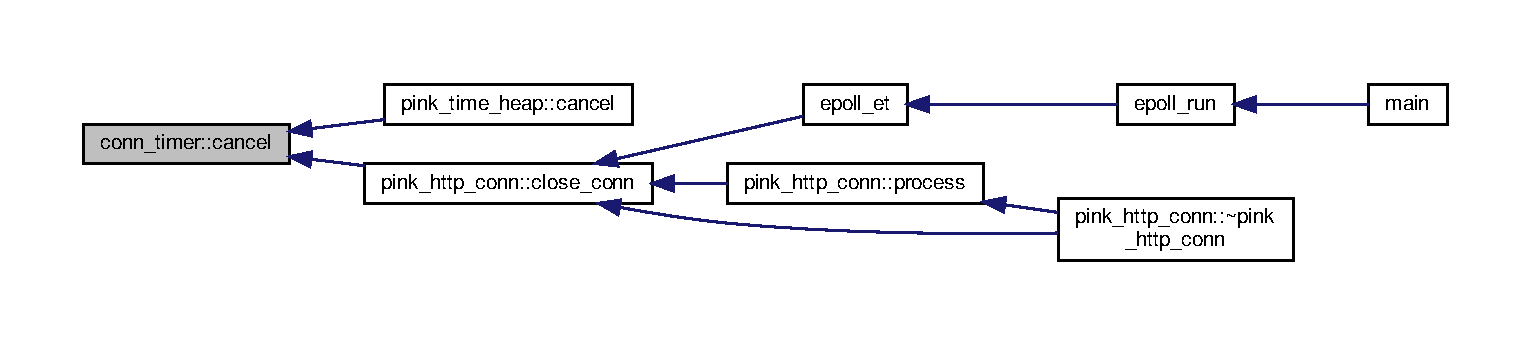
\includegraphics[width=350pt]{classconn__timer_a543102358beb1bc590006310556182de_icgraph}
\end{center}
\end{figure}
\mbox{\Hypertarget{classconn__timer_a86d7a0d33b7423368bba281a0d0eaab9}\label{classconn__timer_a86d7a0d33b7423368bba281a0d0eaab9}} 
\index{conn\+\_\+timer@{conn\+\_\+timer}!cb\+\_\+func@{cb\+\_\+func}}
\index{cb\+\_\+func@{cb\+\_\+func}!conn\+\_\+timer@{conn\+\_\+timer}}
\subsubsection{\texorpdfstring{cb\+\_\+func()}{cb\_func()}}
{\footnotesize\ttfamily void conn\+\_\+timer\+::cb\+\_\+func (\begin{DoxyParamCaption}{ }\end{DoxyParamCaption})\hspace{0.3cm}{\ttfamily [inline]}}



Definition at line 16 of file pink\+\_\+conn\+\_\+timer.\+h.

Here is the caller graph for this function\+:
\nopagebreak
\begin{figure}[H]
\begin{center}
\leavevmode
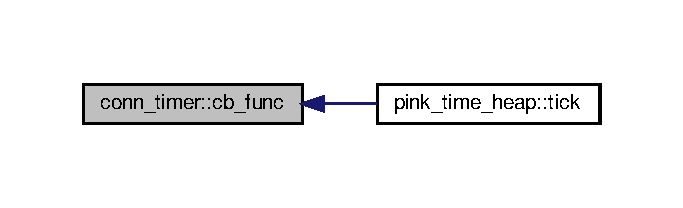
\includegraphics[width=328pt]{classconn__timer_a86d7a0d33b7423368bba281a0d0eaab9_icgraph}
\end{center}
\end{figure}
\mbox{\Hypertarget{classconn__timer_a6cb5ef510c4022acd31b002e15758d60}\label{classconn__timer_a6cb5ef510c4022acd31b002e15758d60}} 
\index{conn\+\_\+timer@{conn\+\_\+timer}!reset@{reset}}
\index{reset@{reset}!conn\+\_\+timer@{conn\+\_\+timer}}
\subsubsection{\texorpdfstring{reset()}{reset()}}
{\footnotesize\ttfamily void conn\+\_\+timer\+::reset (\begin{DoxyParamCaption}\item[{int}]{delay }\end{DoxyParamCaption})\hspace{0.3cm}{\ttfamily [inline]}}



Definition at line 17 of file pink\+\_\+conn\+\_\+timer.\+h.

Here is the caller graph for this function\+:
\nopagebreak
\begin{figure}[H]
\begin{center}
\leavevmode
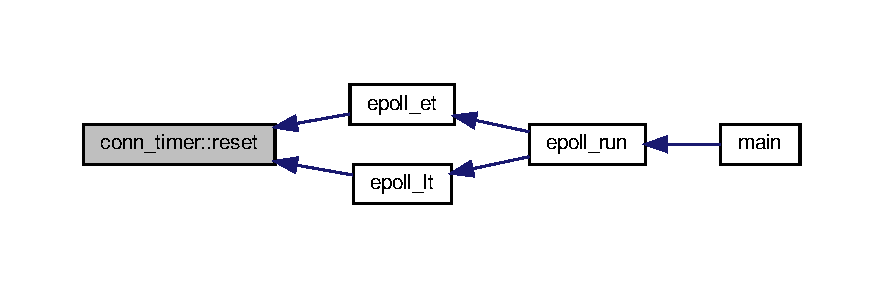
\includegraphics[width=350pt]{classconn__timer_a6cb5ef510c4022acd31b002e15758d60_icgraph}
\end{center}
\end{figure}


\subsection{Member Data Documentation}
\mbox{\Hypertarget{classconn__timer_a51dd2abd61d07bd63c37551404851bf5}\label{classconn__timer_a51dd2abd61d07bd63c37551404851bf5}} 
\index{conn\+\_\+timer@{conn\+\_\+timer}!canceled@{canceled}}
\index{canceled@{canceled}!conn\+\_\+timer@{conn\+\_\+timer}}
\subsubsection{\texorpdfstring{canceled}{canceled}}
{\footnotesize\ttfamily bool conn\+\_\+timer\+::canceled}



Definition at line 23 of file pink\+\_\+conn\+\_\+timer.\+h.

\mbox{\Hypertarget{classconn__timer_a0f3fbb63bdf0764fffe4b5fd0fedc3db}\label{classconn__timer_a0f3fbb63bdf0764fffe4b5fd0fedc3db}} 
\index{conn\+\_\+timer@{conn\+\_\+timer}!conn\+\_\+timeout@{conn\+\_\+timeout}}
\index{conn\+\_\+timeout@{conn\+\_\+timeout}!conn\+\_\+timer@{conn\+\_\+timer}}
\subsubsection{\texorpdfstring{conn\+\_\+timeout}{conn\_timeout}}
{\footnotesize\ttfamily bool$\ast$ conn\+\_\+timer\+::conn\+\_\+timeout}



Definition at line 24 of file pink\+\_\+conn\+\_\+timer.\+h.

\mbox{\Hypertarget{classconn__timer_a2c71b17e51d75dc27a4e0f1f7e443ec5}\label{classconn__timer_a2c71b17e51d75dc27a4e0f1f7e443ec5}} 
\index{conn\+\_\+timer@{conn\+\_\+timer}!expire@{expire}}
\index{expire@{expire}!conn\+\_\+timer@{conn\+\_\+timer}}
\subsubsection{\texorpdfstring{expire}{expire}}
{\footnotesize\ttfamily time\+\_\+t conn\+\_\+timer\+::expire}



Definition at line 22 of file pink\+\_\+conn\+\_\+timer.\+h.



The documentation for this class was generated from the following file\+:\begin{DoxyCompactItemize}
\item 
\hyperlink{pink__conn__timer_8h}{pink\+\_\+conn\+\_\+timer.\+h}\end{DoxyCompactItemize}

\hypertarget{classmutex}{}\section{mutex Class Reference}
\label{classmutex}\index{mutex@{mutex}}


{\ttfamily \#include $<$I\+P\+C\+\_\+tool.\+h$>$}

\subsection*{Public Member Functions}
\begin{DoxyCompactItemize}
\item 
\hyperlink{classmutex_a6b7350155befa79a8c6ad27c4c794b1e}{mutex} ()
\item 
\hyperlink{classmutex_ae30185d87a48c5451a04c2861ba3d034}{$\sim$mutex} ()
\item 
bool \hyperlink{classmutex_afc56ba139d699d2d9d388141209c6e43}{lock} ()
\item 
bool \hyperlink{classmutex_a47bc4d60f08056af411b57e321959fe1}{unlock} ()
\end{DoxyCompactItemize}


\subsection{Detailed Description}


Definition at line 33 of file I\+P\+C\+\_\+tool.\+h.



\subsection{Constructor \& Destructor Documentation}
\mbox{\Hypertarget{classmutex_a6b7350155befa79a8c6ad27c4c794b1e}\label{classmutex_a6b7350155befa79a8c6ad27c4c794b1e}} 
\index{mutex@{mutex}!mutex@{mutex}}
\index{mutex@{mutex}!mutex@{mutex}}
\subsubsection{\texorpdfstring{mutex()}{mutex()}}
{\footnotesize\ttfamily mutex\+::mutex (\begin{DoxyParamCaption}{ }\end{DoxyParamCaption})\hspace{0.3cm}{\ttfamily [inline]}}



Definition at line 35 of file I\+P\+C\+\_\+tool.\+h.

\mbox{\Hypertarget{classmutex_ae30185d87a48c5451a04c2861ba3d034}\label{classmutex_ae30185d87a48c5451a04c2861ba3d034}} 
\index{mutex@{mutex}!````~mutex@{$\sim$mutex}}
\index{````~mutex@{$\sim$mutex}!mutex@{mutex}}
\subsubsection{\texorpdfstring{$\sim$mutex()}{~mutex()}}
{\footnotesize\ttfamily mutex\+::$\sim$mutex (\begin{DoxyParamCaption}{ }\end{DoxyParamCaption})\hspace{0.3cm}{\ttfamily [inline]}}



Definition at line 41 of file I\+P\+C\+\_\+tool.\+h.



\subsection{Member Function Documentation}
\mbox{\Hypertarget{classmutex_afc56ba139d699d2d9d388141209c6e43}\label{classmutex_afc56ba139d699d2d9d388141209c6e43}} 
\index{mutex@{mutex}!lock@{lock}}
\index{lock@{lock}!mutex@{mutex}}
\subsubsection{\texorpdfstring{lock()}{lock()}}
{\footnotesize\ttfamily bool mutex\+::lock (\begin{DoxyParamCaption}{ }\end{DoxyParamCaption})\hspace{0.3cm}{\ttfamily [inline]}}



Definition at line 44 of file I\+P\+C\+\_\+tool.\+h.

Here is the caller graph for this function\+:\nopagebreak
\begin{figure}[H]
\begin{center}
\leavevmode
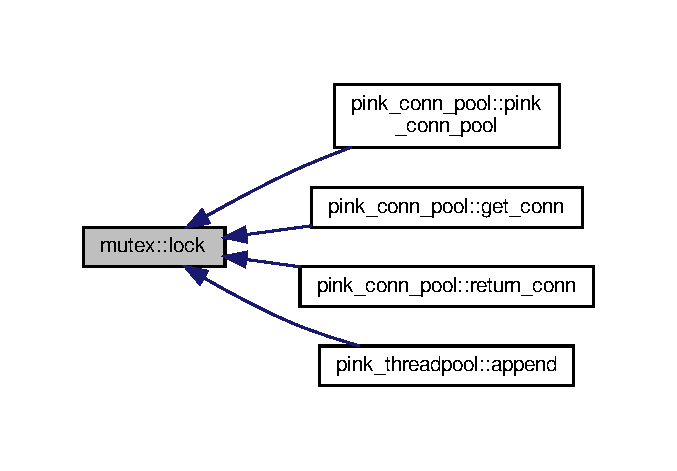
\includegraphics[width=325pt]{classmutex_afc56ba139d699d2d9d388141209c6e43_icgraph}
\end{center}
\end{figure}
\mbox{\Hypertarget{classmutex_a47bc4d60f08056af411b57e321959fe1}\label{classmutex_a47bc4d60f08056af411b57e321959fe1}} 
\index{mutex@{mutex}!unlock@{unlock}}
\index{unlock@{unlock}!mutex@{mutex}}
\subsubsection{\texorpdfstring{unlock()}{unlock()}}
{\footnotesize\ttfamily bool mutex\+::unlock (\begin{DoxyParamCaption}{ }\end{DoxyParamCaption})\hspace{0.3cm}{\ttfamily [inline]}}



Definition at line 47 of file I\+P\+C\+\_\+tool.\+h.

Here is the caller graph for this function\+:\nopagebreak
\begin{figure}[H]
\begin{center}
\leavevmode
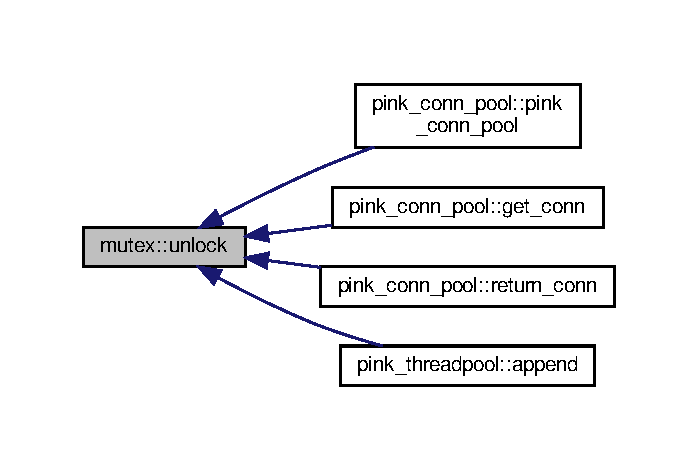
\includegraphics[width=335pt]{classmutex_a47bc4d60f08056af411b57e321959fe1_icgraph}
\end{center}
\end{figure}


The documentation for this class was generated from the following file\+:\begin{DoxyCompactItemize}
\item 
tools/\hyperlink{_i_p_c__tool_8h}{I\+P\+C\+\_\+tool.\+h}\end{DoxyCompactItemize}

\hypertarget{classpink__conn__pool}{}\section{pink\+\_\+conn\+\_\+pool$<$ T $>$ Class Template Reference}
\label{classpink__conn__pool}\index{pink\+\_\+conn\+\_\+pool$<$ T $>$@{pink\+\_\+conn\+\_\+pool$<$ T $>$}}
\subsection*{Public Member Functions}
\begin{DoxyCompactItemize}
\item 
\mbox{\Hypertarget{classpink__conn__pool_a5c557c48815d595f7897f6abc8e55758}\label{classpink__conn__pool_a5c557c48815d595f7897f6abc8e55758}} 
{\bfseries pink\+\_\+conn\+\_\+pool} (int init\+\_\+cur\+\_\+number, int init\+\_\+max\+\_\+number)
\item 
\mbox{\Hypertarget{classpink__conn__pool_a1b053641006c7f00fd4764fea40f410c}\label{classpink__conn__pool_a1b053641006c7f00fd4764fea40f410c}} 
T $\ast$ {\bfseries get\+\_\+conn} ()
\item 
\mbox{\Hypertarget{classpink__conn__pool_a331df25708f142559d051ab8859ed707}\label{classpink__conn__pool_a331df25708f142559d051ab8859ed707}} 
void {\bfseries return\+\_\+conn} (T $\ast$conn)
\item 
\mbox{\Hypertarget{classpink__conn__pool_a90965493d13fc28f0060ca6fed7d12a4}\label{classpink__conn__pool_a90965493d13fc28f0060ca6fed7d12a4}} 
int {\bfseries get\+\_\+used\+\_\+number} ()
\end{DoxyCompactItemize}


The documentation for this class was generated from the following file\+:\begin{DoxyCompactItemize}
\item 
pink\+\_\+conn\+\_\+pool.\+h\end{DoxyCompactItemize}

\hypertarget{classpink__http__conn}{}\section{pink\+\_\+http\+\_\+conn Class Reference}
\label{classpink__http__conn}\index{pink\+\_\+http\+\_\+conn@{pink\+\_\+http\+\_\+conn}}


{\ttfamily \#include $<$pink\+\_\+http\+\_\+conn.\+h$>$}



Collaboration diagram for pink\+\_\+http\+\_\+conn\+:\nopagebreak
\begin{figure}[H]
\begin{center}
\leavevmode
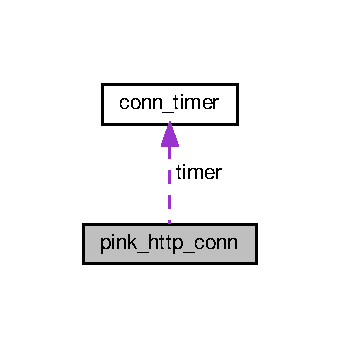
\includegraphics[width=163pt]{classpink__http__conn__coll__graph}
\end{center}
\end{figure}
\subsection*{Public Types}
\begin{DoxyCompactItemize}
\item 
enum \hyperlink{classpink__http__conn_a7959fd18f89efd188dcbc662ff65ddcb}{O\+P\+\_\+\+T\+Y\+PE} \{ \hyperlink{classpink__http__conn_a7959fd18f89efd188dcbc662ff65ddcba811e1ebb2bb8557c98390936e96af25e}{R\+E\+AD} = 0, 
\hyperlink{classpink__http__conn_a7959fd18f89efd188dcbc662ff65ddcba36bef4cc85522d8b97cabc2a031d5dfd}{W\+R\+I\+TE}
 \}
\end{DoxyCompactItemize}
\subsection*{Public Member Functions}
\begin{DoxyCompactItemize}
\item 
\hyperlink{classpink__http__conn_afd3fc76ed1b043d5041741081a2c38ee}{pink\+\_\+http\+\_\+conn} ()
\item 
\hyperlink{classpink__http__conn_a83eb4a1a4b8afdc6bfa0959da37f0e91}{$\sim$pink\+\_\+http\+\_\+conn} ()
\item 
void \hyperlink{classpink__http__conn_abff27697496d209cdc7375f99117f018}{init} (int sockfd, const sockaddr\+\_\+in \&addr)
\item 
void \hyperlink{classpink__http__conn_a14ed30d2643f52ec95c45b11b13b2411}{init\+\_\+listen} (int sockfd)
\item 
void \hyperlink{classpink__http__conn_abdcd7c0da8072d62cb7212523f20298b}{close\+\_\+conn} ()
\item 
void \hyperlink{classpink__http__conn_a41ca12d76d0056562633f27d456d0b62}{process} (int flag)
\item 
bool \hyperlink{classpink__http__conn_a254c09e8b962e5a0bc116f8da271b5ed}{read} ()
\item 
bool \hyperlink{classpink__http__conn_a362df085394bbf2818c8af93932c80d5}{write} ()
\item 
int \hyperlink{classpink__http__conn_aa304899ec9a7f6d7a2a9d738309a9570}{get\+\_\+fd} ()
\end{DoxyCompactItemize}
\subsection*{Public Attributes}
\begin{DoxyCompactItemize}
\item 
\hyperlink{classconn__timer}{conn\+\_\+timer} $\ast$ \hyperlink{classpink__http__conn_a0b34c6a8a6b8f65fa882adb109990e43}{timer}
\item 
bool \hyperlink{classpink__http__conn_a8687eb679249e4ae085c319dd2d4dfc7}{timeout}
\end{DoxyCompactItemize}
\subsection*{Static Public Attributes}
\begin{DoxyCompactItemize}
\item 
static void($\ast$ \hyperlink{classpink__http__conn_a36a48a19aa593001494eb51106628ebd}{delete\+\_\+cb\+\_\+func} )(\hyperlink{classpink__http__conn}{pink\+\_\+http\+\_\+conn} $\ast$conn) = nullptr
\item 
static const int \hyperlink{classpink__http__conn_a240ddaa8b2707d66601b1b82c002ef96}{R\+E\+A\+D\+\_\+\+B\+U\+F\+F\+E\+R\+\_\+\+S\+I\+ZE} = 2048
\item 
static const int \hyperlink{classpink__http__conn_a7764e0564be1e1ae66c44cf34550efea}{W\+R\+I\+T\+E\+\_\+\+B\+U\+F\+F\+E\+R\+\_\+\+S\+I\+ZE} = 1024
\item 
static int \hyperlink{classpink__http__conn_a106c011c818e2a80dbb14c61abbe9a2a}{epollfd} = -\/1
\item 
static int \hyperlink{classpink__http__conn_a4796952e9f7dc2a940e5681bc8f04139}{user\+\_\+count} = 0
\end{DoxyCompactItemize}


\subsection{Detailed Description}


Definition at line 15 of file pink\+\_\+http\+\_\+conn.\+h.



\subsection{Member Enumeration Documentation}
\mbox{\Hypertarget{classpink__http__conn_a7959fd18f89efd188dcbc662ff65ddcb}\label{classpink__http__conn_a7959fd18f89efd188dcbc662ff65ddcb}} 
\index{pink\+\_\+http\+\_\+conn@{pink\+\_\+http\+\_\+conn}!O\+P\+\_\+\+T\+Y\+PE@{O\+P\+\_\+\+T\+Y\+PE}}
\index{O\+P\+\_\+\+T\+Y\+PE@{O\+P\+\_\+\+T\+Y\+PE}!pink\+\_\+http\+\_\+conn@{pink\+\_\+http\+\_\+conn}}
\subsubsection{\texorpdfstring{O\+P\+\_\+\+T\+Y\+PE}{OP\_TYPE}}
{\footnotesize\ttfamily enum \hyperlink{classpink__http__conn_a7959fd18f89efd188dcbc662ff65ddcb}{pink\+\_\+http\+\_\+conn\+::\+O\+P\+\_\+\+T\+Y\+PE}}

\begin{DoxyEnumFields}{Enumerator}
\raisebox{\heightof{T}}[0pt][0pt]{\index{R\+E\+AD@{R\+E\+AD}!pink\+\_\+http\+\_\+conn@{pink\+\_\+http\+\_\+conn}}\index{pink\+\_\+http\+\_\+conn@{pink\+\_\+http\+\_\+conn}!R\+E\+AD@{R\+E\+AD}}}\mbox{\Hypertarget{classpink__http__conn_a7959fd18f89efd188dcbc662ff65ddcba811e1ebb2bb8557c98390936e96af25e}\label{classpink__http__conn_a7959fd18f89efd188dcbc662ff65ddcba811e1ebb2bb8557c98390936e96af25e}} 
R\+E\+AD&\\
\hline

\raisebox{\heightof{T}}[0pt][0pt]{\index{W\+R\+I\+TE@{W\+R\+I\+TE}!pink\+\_\+http\+\_\+conn@{pink\+\_\+http\+\_\+conn}}\index{pink\+\_\+http\+\_\+conn@{pink\+\_\+http\+\_\+conn}!W\+R\+I\+TE@{W\+R\+I\+TE}}}\mbox{\Hypertarget{classpink__http__conn_a7959fd18f89efd188dcbc662ff65ddcba36bef4cc85522d8b97cabc2a031d5dfd}\label{classpink__http__conn_a7959fd18f89efd188dcbc662ff65ddcba36bef4cc85522d8b97cabc2a031d5dfd}} 
W\+R\+I\+TE&\\
\hline

\end{DoxyEnumFields}


Definition at line 35 of file pink\+\_\+http\+\_\+conn.\+h.



\subsection{Constructor \& Destructor Documentation}
\mbox{\Hypertarget{classpink__http__conn_afd3fc76ed1b043d5041741081a2c38ee}\label{classpink__http__conn_afd3fc76ed1b043d5041741081a2c38ee}} 
\index{pink\+\_\+http\+\_\+conn@{pink\+\_\+http\+\_\+conn}!pink\+\_\+http\+\_\+conn@{pink\+\_\+http\+\_\+conn}}
\index{pink\+\_\+http\+\_\+conn@{pink\+\_\+http\+\_\+conn}!pink\+\_\+http\+\_\+conn@{pink\+\_\+http\+\_\+conn}}
\subsubsection{\texorpdfstring{pink\+\_\+http\+\_\+conn()}{pink\_http\_conn()}}
{\footnotesize\ttfamily pink\+\_\+http\+\_\+conn\+::pink\+\_\+http\+\_\+conn (\begin{DoxyParamCaption}{ }\end{DoxyParamCaption})\hspace{0.3cm}{\ttfamily [inline]}}



Definition at line 17 of file pink\+\_\+http\+\_\+conn.\+h.

\mbox{\Hypertarget{classpink__http__conn_a83eb4a1a4b8afdc6bfa0959da37f0e91}\label{classpink__http__conn_a83eb4a1a4b8afdc6bfa0959da37f0e91}} 
\index{pink\+\_\+http\+\_\+conn@{pink\+\_\+http\+\_\+conn}!````~pink\+\_\+http\+\_\+conn@{$\sim$pink\+\_\+http\+\_\+conn}}
\index{````~pink\+\_\+http\+\_\+conn@{$\sim$pink\+\_\+http\+\_\+conn}!pink\+\_\+http\+\_\+conn@{pink\+\_\+http\+\_\+conn}}
\subsubsection{\texorpdfstring{$\sim$pink\+\_\+http\+\_\+conn()}{~pink\_http\_conn()}}
{\footnotesize\ttfamily pink\+\_\+http\+\_\+conn\+::$\sim$pink\+\_\+http\+\_\+conn (\begin{DoxyParamCaption}{ }\end{DoxyParamCaption})\hspace{0.3cm}{\ttfamily [inline]}}



Definition at line 18 of file pink\+\_\+http\+\_\+conn.\+h.

Here is the call graph for this function\+:\nopagebreak
\begin{figure}[H]
\begin{center}
\leavevmode
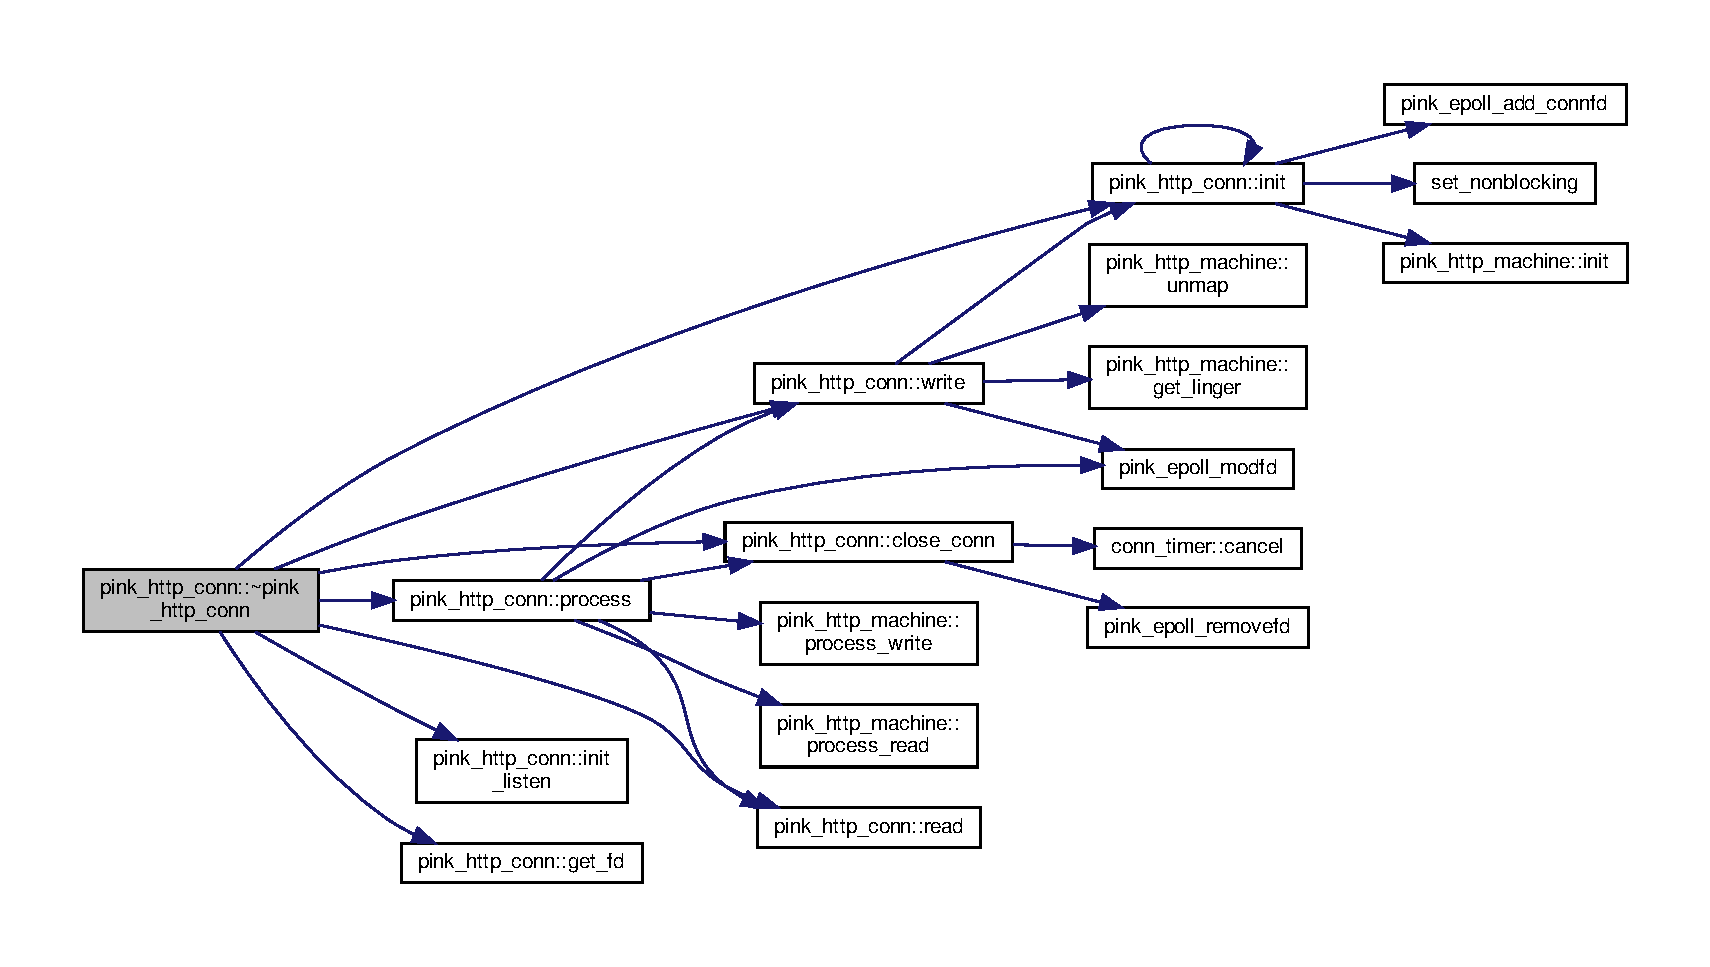
\includegraphics[width=350pt]{classpink__http__conn_a83eb4a1a4b8afdc6bfa0959da37f0e91_cgraph}
\end{center}
\end{figure}


\subsection{Member Function Documentation}
\mbox{\Hypertarget{classpink__http__conn_abdcd7c0da8072d62cb7212523f20298b}\label{classpink__http__conn_abdcd7c0da8072d62cb7212523f20298b}} 
\index{pink\+\_\+http\+\_\+conn@{pink\+\_\+http\+\_\+conn}!close\+\_\+conn@{close\+\_\+conn}}
\index{close\+\_\+conn@{close\+\_\+conn}!pink\+\_\+http\+\_\+conn@{pink\+\_\+http\+\_\+conn}}
\subsubsection{\texorpdfstring{close\+\_\+conn()}{close\_conn()}}
{\footnotesize\ttfamily void pink\+\_\+http\+\_\+conn\+::close\+\_\+conn (\begin{DoxyParamCaption}{ }\end{DoxyParamCaption})}



Definition at line 11 of file pink\+\_\+http\+\_\+conn.\+cpp.

Here is the call graph for this function\+:\nopagebreak
\begin{figure}[H]
\begin{center}
\leavevmode
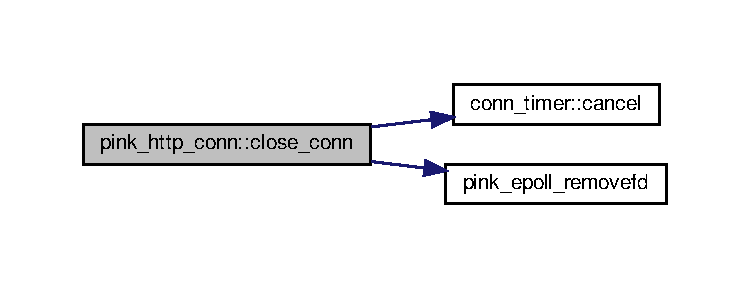
\includegraphics[width=350pt]{classpink__http__conn_abdcd7c0da8072d62cb7212523f20298b_cgraph}
\end{center}
\end{figure}
Here is the caller graph for this function\+:
\nopagebreak
\begin{figure}[H]
\begin{center}
\leavevmode
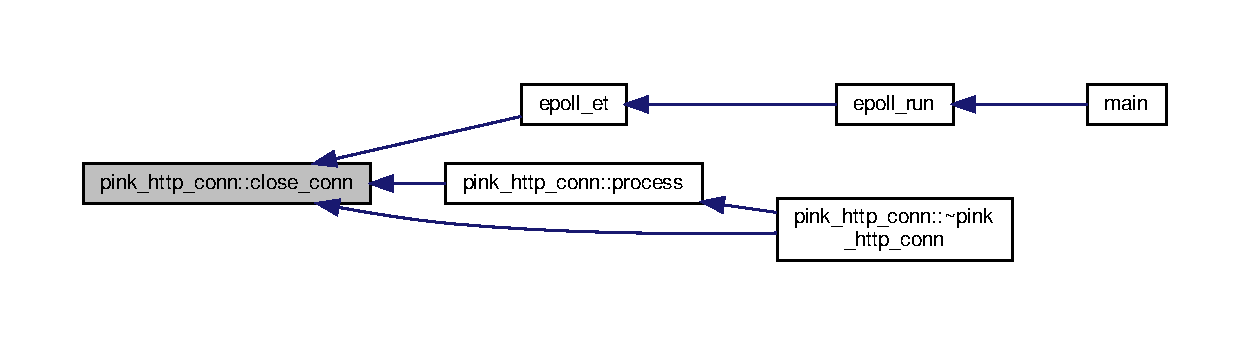
\includegraphics[width=350pt]{classpink__http__conn_abdcd7c0da8072d62cb7212523f20298b_icgraph}
\end{center}
\end{figure}
\mbox{\Hypertarget{classpink__http__conn_aa304899ec9a7f6d7a2a9d738309a9570}\label{classpink__http__conn_aa304899ec9a7f6d7a2a9d738309a9570}} 
\index{pink\+\_\+http\+\_\+conn@{pink\+\_\+http\+\_\+conn}!get\+\_\+fd@{get\+\_\+fd}}
\index{get\+\_\+fd@{get\+\_\+fd}!pink\+\_\+http\+\_\+conn@{pink\+\_\+http\+\_\+conn}}
\subsubsection{\texorpdfstring{get\+\_\+fd()}{get\_fd()}}
{\footnotesize\ttfamily int pink\+\_\+http\+\_\+conn\+::get\+\_\+fd (\begin{DoxyParamCaption}{ }\end{DoxyParamCaption})}



Definition at line 7 of file pink\+\_\+http\+\_\+conn.\+cpp.

Here is the caller graph for this function\+:
\nopagebreak
\begin{figure}[H]
\begin{center}
\leavevmode
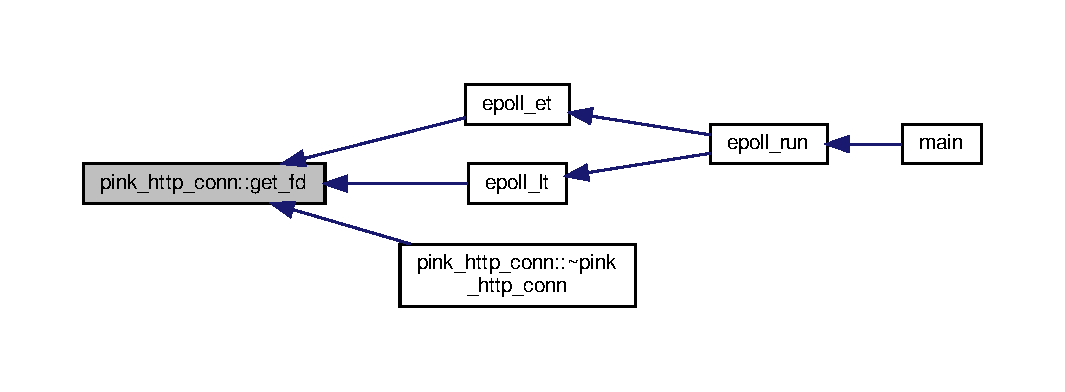
\includegraphics[width=350pt]{classpink__http__conn_aa304899ec9a7f6d7a2a9d738309a9570_icgraph}
\end{center}
\end{figure}
\mbox{\Hypertarget{classpink__http__conn_abff27697496d209cdc7375f99117f018}\label{classpink__http__conn_abff27697496d209cdc7375f99117f018}} 
\index{pink\+\_\+http\+\_\+conn@{pink\+\_\+http\+\_\+conn}!init@{init}}
\index{init@{init}!pink\+\_\+http\+\_\+conn@{pink\+\_\+http\+\_\+conn}}
\subsubsection{\texorpdfstring{init()}{init()}}
{\footnotesize\ttfamily void pink\+\_\+http\+\_\+conn\+::init (\begin{DoxyParamCaption}\item[{int}]{sockfd,  }\item[{const sockaddr\+\_\+in \&}]{addr }\end{DoxyParamCaption})}



Definition at line 25 of file pink\+\_\+http\+\_\+conn.\+cpp.

Here is the call graph for this function\+:
\nopagebreak
\begin{figure}[H]
\begin{center}
\leavevmode
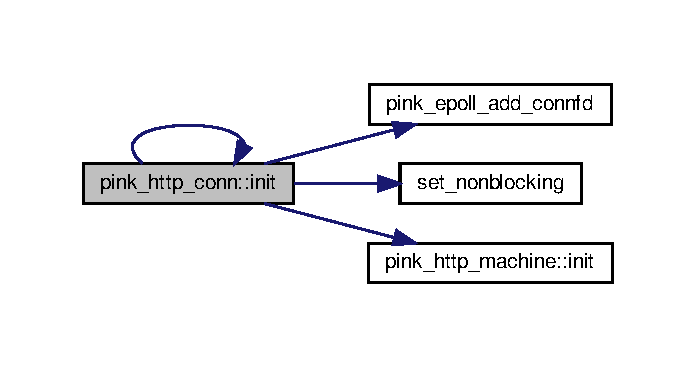
\includegraphics[width=334pt]{classpink__http__conn_abff27697496d209cdc7375f99117f018_cgraph}
\end{center}
\end{figure}
Here is the caller graph for this function\+:
\nopagebreak
\begin{figure}[H]
\begin{center}
\leavevmode
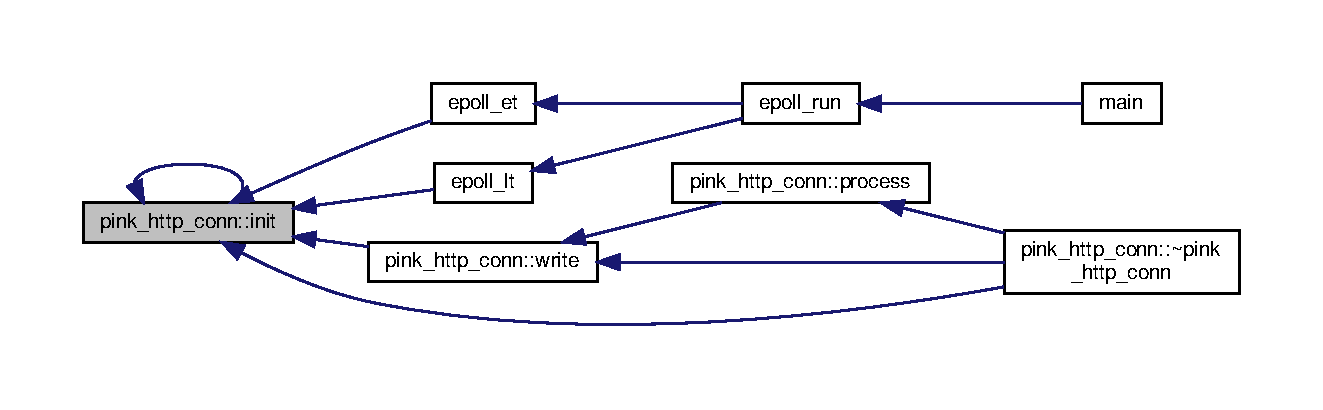
\includegraphics[width=350pt]{classpink__http__conn_abff27697496d209cdc7375f99117f018_icgraph}
\end{center}
\end{figure}
\mbox{\Hypertarget{classpink__http__conn_a14ed30d2643f52ec95c45b11b13b2411}\label{classpink__http__conn_a14ed30d2643f52ec95c45b11b13b2411}} 
\index{pink\+\_\+http\+\_\+conn@{pink\+\_\+http\+\_\+conn}!init\+\_\+listen@{init\+\_\+listen}}
\index{init\+\_\+listen@{init\+\_\+listen}!pink\+\_\+http\+\_\+conn@{pink\+\_\+http\+\_\+conn}}
\subsubsection{\texorpdfstring{init\+\_\+listen()}{init\_listen()}}
{\footnotesize\ttfamily void pink\+\_\+http\+\_\+conn\+::init\+\_\+listen (\begin{DoxyParamCaption}\item[{int}]{sockfd }\end{DoxyParamCaption})}



Definition at line 21 of file pink\+\_\+http\+\_\+conn.\+cpp.

Here is the caller graph for this function\+:
\nopagebreak
\begin{figure}[H]
\begin{center}
\leavevmode
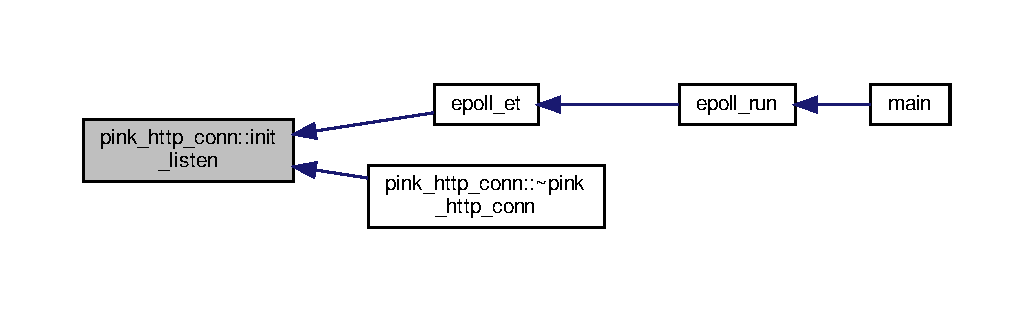
\includegraphics[width=350pt]{classpink__http__conn_a14ed30d2643f52ec95c45b11b13b2411_icgraph}
\end{center}
\end{figure}
\mbox{\Hypertarget{classpink__http__conn_a41ca12d76d0056562633f27d456d0b62}\label{classpink__http__conn_a41ca12d76d0056562633f27d456d0b62}} 
\index{pink\+\_\+http\+\_\+conn@{pink\+\_\+http\+\_\+conn}!process@{process}}
\index{process@{process}!pink\+\_\+http\+\_\+conn@{pink\+\_\+http\+\_\+conn}}
\subsubsection{\texorpdfstring{process()}{process()}}
{\footnotesize\ttfamily void pink\+\_\+http\+\_\+conn\+::process (\begin{DoxyParamCaption}\item[{int}]{flag }\end{DoxyParamCaption})}



Definition at line 54 of file pink\+\_\+http\+\_\+conn.\+cpp.

Here is the call graph for this function\+:
\nopagebreak
\begin{figure}[H]
\begin{center}
\leavevmode
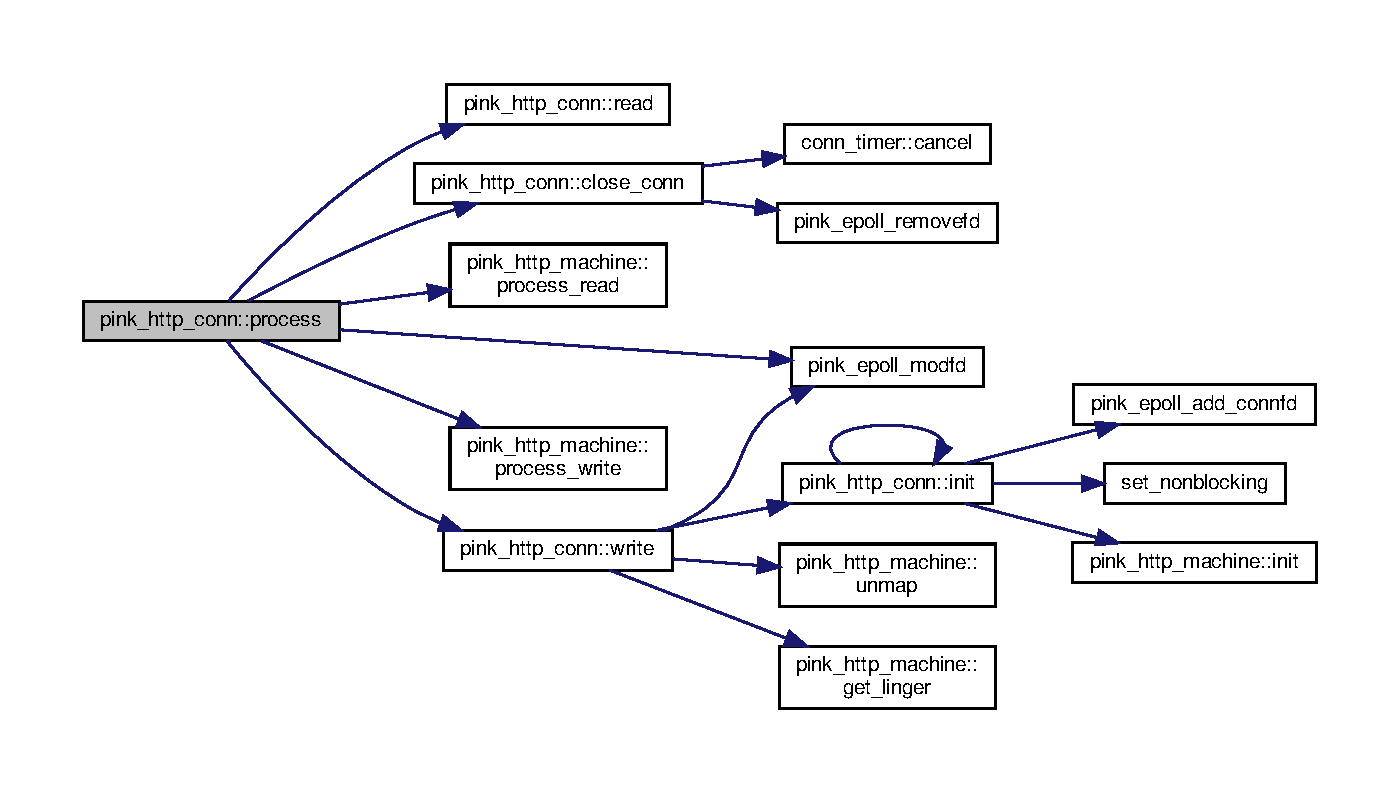
\includegraphics[width=350pt]{classpink__http__conn_a41ca12d76d0056562633f27d456d0b62_cgraph}
\end{center}
\end{figure}
Here is the caller graph for this function\+:
\nopagebreak
\begin{figure}[H]
\begin{center}
\leavevmode
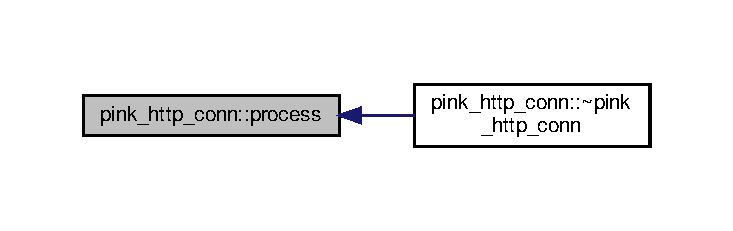
\includegraphics[width=350pt]{classpink__http__conn_a41ca12d76d0056562633f27d456d0b62_icgraph}
\end{center}
\end{figure}
\mbox{\Hypertarget{classpink__http__conn_a254c09e8b962e5a0bc116f8da271b5ed}\label{classpink__http__conn_a254c09e8b962e5a0bc116f8da271b5ed}} 
\index{pink\+\_\+http\+\_\+conn@{pink\+\_\+http\+\_\+conn}!read@{read}}
\index{read@{read}!pink\+\_\+http\+\_\+conn@{pink\+\_\+http\+\_\+conn}}
\subsubsection{\texorpdfstring{read()}{read()}}
{\footnotesize\ttfamily bool pink\+\_\+http\+\_\+conn\+::read (\begin{DoxyParamCaption}{ }\end{DoxyParamCaption})}



Definition at line 87 of file pink\+\_\+http\+\_\+conn.\+cpp.

Here is the caller graph for this function\+:
\nopagebreak
\begin{figure}[H]
\begin{center}
\leavevmode
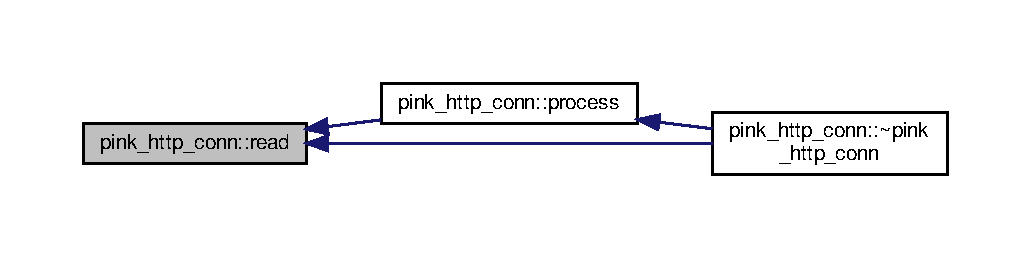
\includegraphics[width=350pt]{classpink__http__conn_a254c09e8b962e5a0bc116f8da271b5ed_icgraph}
\end{center}
\end{figure}
\mbox{\Hypertarget{classpink__http__conn_a362df085394bbf2818c8af93932c80d5}\label{classpink__http__conn_a362df085394bbf2818c8af93932c80d5}} 
\index{pink\+\_\+http\+\_\+conn@{pink\+\_\+http\+\_\+conn}!write@{write}}
\index{write@{write}!pink\+\_\+http\+\_\+conn@{pink\+\_\+http\+\_\+conn}}
\subsubsection{\texorpdfstring{write()}{write()}}
{\footnotesize\ttfamily bool pink\+\_\+http\+\_\+conn\+::write (\begin{DoxyParamCaption}{ }\end{DoxyParamCaption})}



Definition at line 112 of file pink\+\_\+http\+\_\+conn.\+cpp.

Here is the call graph for this function\+:
\nopagebreak
\begin{figure}[H]
\begin{center}
\leavevmode
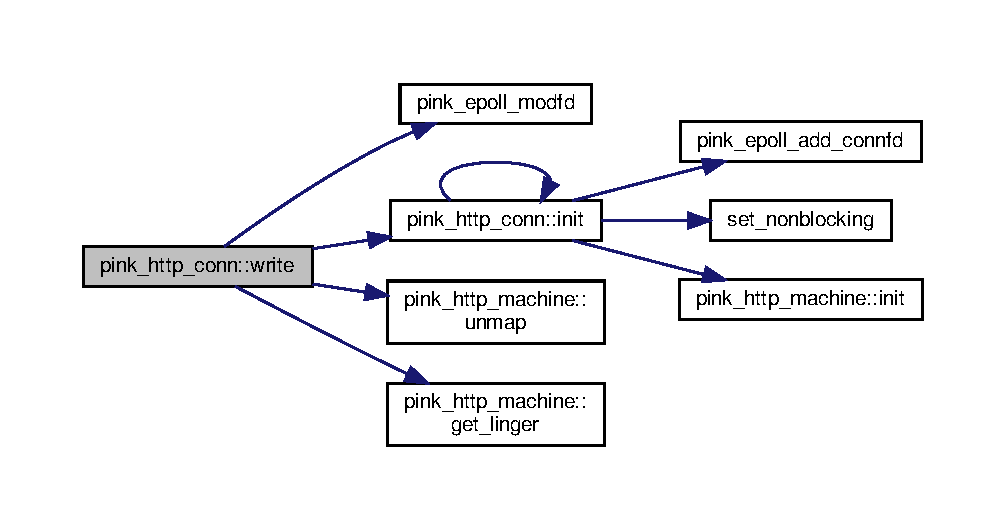
\includegraphics[width=350pt]{classpink__http__conn_a362df085394bbf2818c8af93932c80d5_cgraph}
\end{center}
\end{figure}
Here is the caller graph for this function\+:
\nopagebreak
\begin{figure}[H]
\begin{center}
\leavevmode
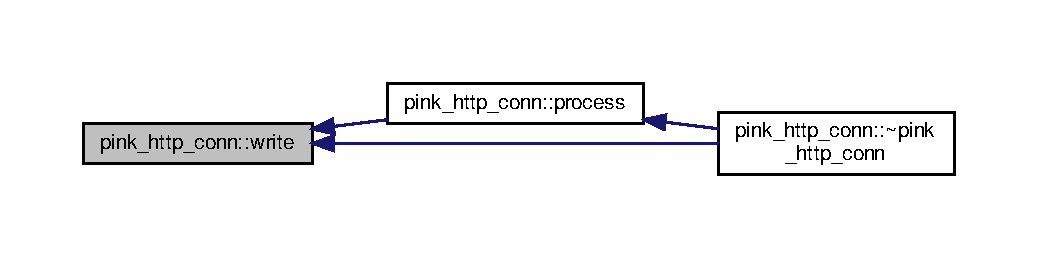
\includegraphics[width=350pt]{classpink__http__conn_a362df085394bbf2818c8af93932c80d5_icgraph}
\end{center}
\end{figure}


\subsection{Member Data Documentation}
\mbox{\Hypertarget{classpink__http__conn_a36a48a19aa593001494eb51106628ebd}\label{classpink__http__conn_a36a48a19aa593001494eb51106628ebd}} 
\index{pink\+\_\+http\+\_\+conn@{pink\+\_\+http\+\_\+conn}!delete\+\_\+cb\+\_\+func@{delete\+\_\+cb\+\_\+func}}
\index{delete\+\_\+cb\+\_\+func@{delete\+\_\+cb\+\_\+func}!pink\+\_\+http\+\_\+conn@{pink\+\_\+http\+\_\+conn}}
\subsubsection{\texorpdfstring{delete\+\_\+cb\+\_\+func}{delete\_cb\_func}}
{\footnotesize\ttfamily void($\ast$ pink\+\_\+http\+\_\+conn\+::delete\+\_\+cb\+\_\+func)(\hyperlink{classpink__http__conn}{pink\+\_\+http\+\_\+conn} $\ast$) = nullptr\hspace{0.3cm}{\ttfamily [static]}}



Definition at line 37 of file pink\+\_\+http\+\_\+conn.\+h.

\mbox{\Hypertarget{classpink__http__conn_a106c011c818e2a80dbb14c61abbe9a2a}\label{classpink__http__conn_a106c011c818e2a80dbb14c61abbe9a2a}} 
\index{pink\+\_\+http\+\_\+conn@{pink\+\_\+http\+\_\+conn}!epollfd@{epollfd}}
\index{epollfd@{epollfd}!pink\+\_\+http\+\_\+conn@{pink\+\_\+http\+\_\+conn}}
\subsubsection{\texorpdfstring{epollfd}{epollfd}}
{\footnotesize\ttfamily int pink\+\_\+http\+\_\+conn\+::epollfd = -\/1\hspace{0.3cm}{\ttfamily [static]}}



Definition at line 46 of file pink\+\_\+http\+\_\+conn.\+h.

\mbox{\Hypertarget{classpink__http__conn_a240ddaa8b2707d66601b1b82c002ef96}\label{classpink__http__conn_a240ddaa8b2707d66601b1b82c002ef96}} 
\index{pink\+\_\+http\+\_\+conn@{pink\+\_\+http\+\_\+conn}!R\+E\+A\+D\+\_\+\+B\+U\+F\+F\+E\+R\+\_\+\+S\+I\+ZE@{R\+E\+A\+D\+\_\+\+B\+U\+F\+F\+E\+R\+\_\+\+S\+I\+ZE}}
\index{R\+E\+A\+D\+\_\+\+B\+U\+F\+F\+E\+R\+\_\+\+S\+I\+ZE@{R\+E\+A\+D\+\_\+\+B\+U\+F\+F\+E\+R\+\_\+\+S\+I\+ZE}!pink\+\_\+http\+\_\+conn@{pink\+\_\+http\+\_\+conn}}
\subsubsection{\texorpdfstring{R\+E\+A\+D\+\_\+\+B\+U\+F\+F\+E\+R\+\_\+\+S\+I\+ZE}{READ\_BUFFER\_SIZE}}
{\footnotesize\ttfamily const int pink\+\_\+http\+\_\+conn\+::\+R\+E\+A\+D\+\_\+\+B\+U\+F\+F\+E\+R\+\_\+\+S\+I\+ZE = 2048\hspace{0.3cm}{\ttfamily [static]}}



Definition at line 44 of file pink\+\_\+http\+\_\+conn.\+h.

\mbox{\Hypertarget{classpink__http__conn_a8687eb679249e4ae085c319dd2d4dfc7}\label{classpink__http__conn_a8687eb679249e4ae085c319dd2d4dfc7}} 
\index{pink\+\_\+http\+\_\+conn@{pink\+\_\+http\+\_\+conn}!timeout@{timeout}}
\index{timeout@{timeout}!pink\+\_\+http\+\_\+conn@{pink\+\_\+http\+\_\+conn}}
\subsubsection{\texorpdfstring{timeout}{timeout}}
{\footnotesize\ttfamily bool pink\+\_\+http\+\_\+conn\+::timeout}



Definition at line 49 of file pink\+\_\+http\+\_\+conn.\+h.

\mbox{\Hypertarget{classpink__http__conn_a0b34c6a8a6b8f65fa882adb109990e43}\label{classpink__http__conn_a0b34c6a8a6b8f65fa882adb109990e43}} 
\index{pink\+\_\+http\+\_\+conn@{pink\+\_\+http\+\_\+conn}!timer@{timer}}
\index{timer@{timer}!pink\+\_\+http\+\_\+conn@{pink\+\_\+http\+\_\+conn}}
\subsubsection{\texorpdfstring{timer}{timer}}
{\footnotesize\ttfamily \hyperlink{classconn__timer}{conn\+\_\+timer}$\ast$ pink\+\_\+http\+\_\+conn\+::timer}



Definition at line 48 of file pink\+\_\+http\+\_\+conn.\+h.

\mbox{\Hypertarget{classpink__http__conn_a4796952e9f7dc2a940e5681bc8f04139}\label{classpink__http__conn_a4796952e9f7dc2a940e5681bc8f04139}} 
\index{pink\+\_\+http\+\_\+conn@{pink\+\_\+http\+\_\+conn}!user\+\_\+count@{user\+\_\+count}}
\index{user\+\_\+count@{user\+\_\+count}!pink\+\_\+http\+\_\+conn@{pink\+\_\+http\+\_\+conn}}
\subsubsection{\texorpdfstring{user\+\_\+count}{user\_count}}
{\footnotesize\ttfamily int pink\+\_\+http\+\_\+conn\+::user\+\_\+count = 0\hspace{0.3cm}{\ttfamily [static]}}



Definition at line 47 of file pink\+\_\+http\+\_\+conn.\+h.

\mbox{\Hypertarget{classpink__http__conn_a7764e0564be1e1ae66c44cf34550efea}\label{classpink__http__conn_a7764e0564be1e1ae66c44cf34550efea}} 
\index{pink\+\_\+http\+\_\+conn@{pink\+\_\+http\+\_\+conn}!W\+R\+I\+T\+E\+\_\+\+B\+U\+F\+F\+E\+R\+\_\+\+S\+I\+ZE@{W\+R\+I\+T\+E\+\_\+\+B\+U\+F\+F\+E\+R\+\_\+\+S\+I\+ZE}}
\index{W\+R\+I\+T\+E\+\_\+\+B\+U\+F\+F\+E\+R\+\_\+\+S\+I\+ZE@{W\+R\+I\+T\+E\+\_\+\+B\+U\+F\+F\+E\+R\+\_\+\+S\+I\+ZE}!pink\+\_\+http\+\_\+conn@{pink\+\_\+http\+\_\+conn}}
\subsubsection{\texorpdfstring{W\+R\+I\+T\+E\+\_\+\+B\+U\+F\+F\+E\+R\+\_\+\+S\+I\+ZE}{WRITE\_BUFFER\_SIZE}}
{\footnotesize\ttfamily const int pink\+\_\+http\+\_\+conn\+::\+W\+R\+I\+T\+E\+\_\+\+B\+U\+F\+F\+E\+R\+\_\+\+S\+I\+ZE = 1024\hspace{0.3cm}{\ttfamily [static]}}



Definition at line 45 of file pink\+\_\+http\+\_\+conn.\+h.



The documentation for this class was generated from the following files\+:\begin{DoxyCompactItemize}
\item 
\hyperlink{pink__http__conn_8h}{pink\+\_\+http\+\_\+conn.\+h}\item 
\hyperlink{pink__http__conn_8cpp}{pink\+\_\+http\+\_\+conn.\+cpp}\end{DoxyCompactItemize}

\hypertarget{classpink__http__machine}{}\section{pink\+\_\+http\+\_\+machine Class Reference}
\label{classpink__http__machine}\index{pink\+\_\+http\+\_\+machine@{pink\+\_\+http\+\_\+machine}}


{\ttfamily \#include $<$pink\+\_\+http\+\_\+machine.\+h$>$}



Collaboration diagram for pink\+\_\+http\+\_\+machine\+:
\nopagebreak
\begin{figure}[H]
\begin{center}
\leavevmode
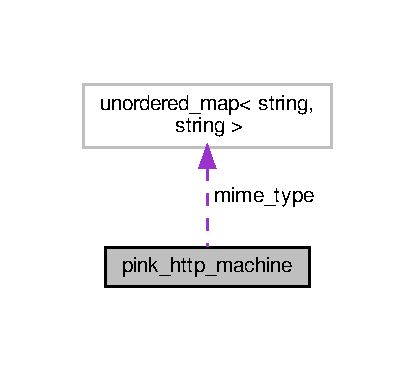
\includegraphics[width=199pt]{classpink__http__machine__coll__graph}
\end{center}
\end{figure}
\subsection*{Public Types}
\begin{DoxyCompactItemize}
\item 
enum \hyperlink{classpink__http__machine_a64bc87fde84112f9e18a09c7d439aa2b}{M\+E\+T\+H\+OD} \{ \newline
\hyperlink{classpink__http__machine_a64bc87fde84112f9e18a09c7d439aa2ba941353ab7fbe8de7c3e211613c832521}{G\+ET} =0, 
\hyperlink{classpink__http__machine_a64bc87fde84112f9e18a09c7d439aa2ba9aac7af48a218454e17ff29dba82f0be}{P\+O\+ST}, 
\hyperlink{classpink__http__machine_a64bc87fde84112f9e18a09c7d439aa2ba32337e87e4cf7dbe8de6241d55b2674b}{H\+E\+AD}, 
\hyperlink{classpink__http__machine_a64bc87fde84112f9e18a09c7d439aa2badee80adbc5551abbeb1bb4c0674f322a}{P\+UT}, 
\newline
\hyperlink{classpink__http__machine_a64bc87fde84112f9e18a09c7d439aa2ba8774cb5bcde90169f21fa72e5d618de7}{D\+E\+L\+E\+TE}, 
\hyperlink{classpink__http__machine_a64bc87fde84112f9e18a09c7d439aa2badcdb9de10fe7689ba1cf313c0de85229}{T\+R\+A\+CE}, 
\hyperlink{classpink__http__machine_a64bc87fde84112f9e18a09c7d439aa2ba0dc30f9df08eed397e07be7cf43af2ea}{O\+P\+T\+I\+O\+NS}, 
\hyperlink{classpink__http__machine_a64bc87fde84112f9e18a09c7d439aa2baeb9d3fcb973b6922d8b1ddb1e6290204}{C\+O\+N\+N\+E\+CT}, 
\newline
\hyperlink{classpink__http__machine_a64bc87fde84112f9e18a09c7d439aa2bad1fda1b7588701be35981d2bdffd3959}{P\+A\+T\+CH}, 
\hyperlink{classpink__http__machine_a64bc87fde84112f9e18a09c7d439aa2bac9ca94619d2ce5c718356d251c7a5127}{U\+N\+K\+N\+O\+W\+N\+\_\+\+M\+E\+T\+H\+OD}
 \}
\item 
enum \hyperlink{classpink__http__machine_aeb5dafe8258708065e5c09565dd37f9e}{C\+H\+E\+C\+K\+\_\+\+S\+T\+A\+TE} \{ \hyperlink{classpink__http__machine_aeb5dafe8258708065e5c09565dd37f9ea45849c7923cca06d5e7a8c2024cb2d1e}{C\+H\+E\+C\+K\+\_\+\+S\+T\+A\+T\+E\+\_\+\+R\+E\+Q\+U\+E\+S\+T\+L\+I\+NE} = 0, 
\hyperlink{classpink__http__machine_aeb5dafe8258708065e5c09565dd37f9eaadc3fa37b117c846fc9bc7b188ce2bfe}{C\+H\+E\+C\+K\+\_\+\+S\+T\+A\+T\+E\+\_\+\+H\+E\+A\+D\+ER}, 
\hyperlink{classpink__http__machine_aeb5dafe8258708065e5c09565dd37f9eac27eaf6929e26d60c742247caf03d0ee}{C\+H\+E\+C\+K\+\_\+\+S\+T\+A\+T\+E\+\_\+\+C\+O\+N\+T\+E\+NT}
 \}
\item 
enum \hyperlink{classpink__http__machine_afb1e590cd61676c2f8859c4e01e5b150}{H\+T\+T\+P\+\_\+\+C\+O\+DE} \{ \newline
\hyperlink{classpink__http__machine_afb1e590cd61676c2f8859c4e01e5b150ab2ca25354e96b87e666a892a1ac8c35c}{N\+O\+T\+\_\+\+C\+O\+M\+P\+L\+E\+T\+ED}, 
\hyperlink{classpink__http__machine_afb1e590cd61676c2f8859c4e01e5b150af80968b6c39c54dff2e5d5541658a374}{G\+E\+T\+\_\+\+R\+E\+Q\+U\+E\+ST}, 
\hyperlink{classpink__http__machine_afb1e590cd61676c2f8859c4e01e5b150a593a224a7435a2c69aec97d827efbb8b}{B\+A\+D\+\_\+\+R\+E\+Q\+U\+E\+ST}, 
\hyperlink{classpink__http__machine_afb1e590cd61676c2f8859c4e01e5b150a0b325eacf5b65952576b6197785e86b9}{N\+O\+\_\+\+R\+E\+S\+O\+U\+R\+CE}, 
\newline
\hyperlink{classpink__http__machine_afb1e590cd61676c2f8859c4e01e5b150aef6f8e15b18fb0bad605acba3ddfd4ad}{F\+O\+R\+B\+I\+D\+D\+E\+N\+\_\+\+R\+E\+Q\+U\+E\+ST}, 
\hyperlink{classpink__http__machine_afb1e590cd61676c2f8859c4e01e5b150a44149cde43145b42953c4825f5d51107}{F\+I\+L\+E\+\_\+\+R\+E\+Q\+U\+E\+ST}, 
\hyperlink{classpink__http__machine_afb1e590cd61676c2f8859c4e01e5b150aa4e2f23c9ddc8e39742256ed3f1725d7}{I\+N\+T\+E\+R\+N\+A\+L\+\_\+\+E\+R\+R\+OR}, 
\hyperlink{classpink__http__machine_afb1e590cd61676c2f8859c4e01e5b150ab3925c78bae06472d9317e9b5e5b68fa}{C\+L\+O\+S\+E\+D\+\_\+\+C\+O\+N\+N\+E\+C\+T\+I\+ON}
 \}
\item 
enum \hyperlink{classpink__http__machine_ab93a9e606b05f96c1b4b0f7079d1e279}{L\+I\+N\+E\+\_\+\+S\+T\+A\+T\+US} \{ \hyperlink{classpink__http__machine_ab93a9e606b05f96c1b4b0f7079d1e279a20dc04aa8adadcff78c8a123f5c311a4}{L\+I\+N\+E\+\_\+\+OK} = 0, 
\hyperlink{classpink__http__machine_ab93a9e606b05f96c1b4b0f7079d1e279a6bf5713029c7f488f44cc8f9ae94ac25}{L\+I\+N\+E\+\_\+\+B\+AD}, 
\hyperlink{classpink__http__machine_ab93a9e606b05f96c1b4b0f7079d1e279a42889372cee61ec858a6ae605284f4f2}{L\+I\+N\+E\+\_\+\+O\+P\+EN}
 \}
\end{DoxyCompactItemize}
\subsection*{Public Member Functions}
\begin{DoxyCompactItemize}
\item 
\hyperlink{classpink__http__machine_a8f5a3d6283cb4e9237cf1deb01548826}{pink\+\_\+http\+\_\+machine} ()
\item 
\hyperlink{classpink__http__machine_a38d1d6228955fc97c752d330d4c126c2}{$\sim$pink\+\_\+http\+\_\+machine} ()
\item 
void \hyperlink{classpink__http__machine_a32b0ee47de1b90467d17194fa83b4eb0}{init} (char $\ast$read\+\_\+buf, char $\ast$write\+\_\+buf, int $\ast$read\+\_\+idx, int $\ast$write\+\_\+idx, const int read\+\_\+buf\+\_\+size, const int write\+\_\+buf\+\_\+size)
\item 
\hyperlink{classpink__http__machine_afb1e590cd61676c2f8859c4e01e5b150}{H\+T\+T\+P\+\_\+\+C\+O\+DE} \hyperlink{classpink__http__machine_a7c937bd8da6bdfbf4894e6af9a712d60}{process\+\_\+read} ()
\item 
bool \hyperlink{classpink__http__machine_a7144e4279cd09ab8ce56873bd3906f24}{process\+\_\+write} (\hyperlink{classpink__http__machine_afb1e590cd61676c2f8859c4e01e5b150}{H\+T\+T\+P\+\_\+\+C\+O\+DE} ret, struct iovec $\ast$iv, int \&iv\+\_\+count)
\item 
void \hyperlink{classpink__http__machine_a26debab8c361df5c79966f11e2b2dd17}{unmap} ()
\item 
bool \hyperlink{classpink__http__machine_a01dcf59a537c21d5a4a92c1c25fbf3ab}{get\+\_\+linger} ()
\end{DoxyCompactItemize}
\subsection*{Static Public Member Functions}
\begin{DoxyCompactItemize}
\item 
static unordered\+\_\+map$<$ string, string $>$ \hyperlink{classpink__http__machine_ad6d404392628f4b2c94a4b30fefb62f8}{mime\+\_\+map\+\_\+init} ()
\end{DoxyCompactItemize}
\subsection*{Static Public Attributes}
\begin{DoxyCompactItemize}
\item 
static constexpr int \hyperlink{classpink__http__machine_a33993ee83910b37ae5672c6e6c94cac3}{F\+I\+L\+E\+N\+A\+M\+E\+\_\+\+L\+EN} = 1024
\item 
static unordered\+\_\+map$<$ string, string $>$ \hyperlink{classpink__http__machine_a4373363c5bd675e182f502d300157aa9}{mime\+\_\+type}
\end{DoxyCompactItemize}


\subsection{Detailed Description}


Definition at line 33 of file pink\+\_\+http\+\_\+machine.\+h.



\subsection{Member Enumeration Documentation}
\mbox{\Hypertarget{classpink__http__machine_aeb5dafe8258708065e5c09565dd37f9e}\label{classpink__http__machine_aeb5dafe8258708065e5c09565dd37f9e}} 
\index{pink\+\_\+http\+\_\+machine@{pink\+\_\+http\+\_\+machine}!C\+H\+E\+C\+K\+\_\+\+S\+T\+A\+TE@{C\+H\+E\+C\+K\+\_\+\+S\+T\+A\+TE}}
\index{C\+H\+E\+C\+K\+\_\+\+S\+T\+A\+TE@{C\+H\+E\+C\+K\+\_\+\+S\+T\+A\+TE}!pink\+\_\+http\+\_\+machine@{pink\+\_\+http\+\_\+machine}}
\subsubsection{\texorpdfstring{C\+H\+E\+C\+K\+\_\+\+S\+T\+A\+TE}{CHECK\_STATE}}
{\footnotesize\ttfamily enum \hyperlink{classpink__http__machine_aeb5dafe8258708065e5c09565dd37f9e}{pink\+\_\+http\+\_\+machine\+::\+C\+H\+E\+C\+K\+\_\+\+S\+T\+A\+TE}}

\begin{DoxyEnumFields}{Enumerator}
\raisebox{\heightof{T}}[0pt][0pt]{\index{C\+H\+E\+C\+K\+\_\+\+S\+T\+A\+T\+E\+\_\+\+R\+E\+Q\+U\+E\+S\+T\+L\+I\+NE@{C\+H\+E\+C\+K\+\_\+\+S\+T\+A\+T\+E\+\_\+\+R\+E\+Q\+U\+E\+S\+T\+L\+I\+NE}!pink\+\_\+http\+\_\+machine@{pink\+\_\+http\+\_\+machine}}\index{pink\+\_\+http\+\_\+machine@{pink\+\_\+http\+\_\+machine}!C\+H\+E\+C\+K\+\_\+\+S\+T\+A\+T\+E\+\_\+\+R\+E\+Q\+U\+E\+S\+T\+L\+I\+NE@{C\+H\+E\+C\+K\+\_\+\+S\+T\+A\+T\+E\+\_\+\+R\+E\+Q\+U\+E\+S\+T\+L\+I\+NE}}}\mbox{\Hypertarget{classpink__http__machine_aeb5dafe8258708065e5c09565dd37f9ea45849c7923cca06d5e7a8c2024cb2d1e}\label{classpink__http__machine_aeb5dafe8258708065e5c09565dd37f9ea45849c7923cca06d5e7a8c2024cb2d1e}} 
C\+H\+E\+C\+K\+\_\+\+S\+T\+A\+T\+E\+\_\+\+R\+E\+Q\+U\+E\+S\+T\+L\+I\+NE&\\
\hline

\raisebox{\heightof{T}}[0pt][0pt]{\index{C\+H\+E\+C\+K\+\_\+\+S\+T\+A\+T\+E\+\_\+\+H\+E\+A\+D\+ER@{C\+H\+E\+C\+K\+\_\+\+S\+T\+A\+T\+E\+\_\+\+H\+E\+A\+D\+ER}!pink\+\_\+http\+\_\+machine@{pink\+\_\+http\+\_\+machine}}\index{pink\+\_\+http\+\_\+machine@{pink\+\_\+http\+\_\+machine}!C\+H\+E\+C\+K\+\_\+\+S\+T\+A\+T\+E\+\_\+\+H\+E\+A\+D\+ER@{C\+H\+E\+C\+K\+\_\+\+S\+T\+A\+T\+E\+\_\+\+H\+E\+A\+D\+ER}}}\mbox{\Hypertarget{classpink__http__machine_aeb5dafe8258708065e5c09565dd37f9eaadc3fa37b117c846fc9bc7b188ce2bfe}\label{classpink__http__machine_aeb5dafe8258708065e5c09565dd37f9eaadc3fa37b117c846fc9bc7b188ce2bfe}} 
C\+H\+E\+C\+K\+\_\+\+S\+T\+A\+T\+E\+\_\+\+H\+E\+A\+D\+ER&\\
\hline

\raisebox{\heightof{T}}[0pt][0pt]{\index{C\+H\+E\+C\+K\+\_\+\+S\+T\+A\+T\+E\+\_\+\+C\+O\+N\+T\+E\+NT@{C\+H\+E\+C\+K\+\_\+\+S\+T\+A\+T\+E\+\_\+\+C\+O\+N\+T\+E\+NT}!pink\+\_\+http\+\_\+machine@{pink\+\_\+http\+\_\+machine}}\index{pink\+\_\+http\+\_\+machine@{pink\+\_\+http\+\_\+machine}!C\+H\+E\+C\+K\+\_\+\+S\+T\+A\+T\+E\+\_\+\+C\+O\+N\+T\+E\+NT@{C\+H\+E\+C\+K\+\_\+\+S\+T\+A\+T\+E\+\_\+\+C\+O\+N\+T\+E\+NT}}}\mbox{\Hypertarget{classpink__http__machine_aeb5dafe8258708065e5c09565dd37f9eac27eaf6929e26d60c742247caf03d0ee}\label{classpink__http__machine_aeb5dafe8258708065e5c09565dd37f9eac27eaf6929e26d60c742247caf03d0ee}} 
C\+H\+E\+C\+K\+\_\+\+S\+T\+A\+T\+E\+\_\+\+C\+O\+N\+T\+E\+NT&\\
\hline

\end{DoxyEnumFields}


Definition at line 40 of file pink\+\_\+http\+\_\+machine.\+h.

\mbox{\Hypertarget{classpink__http__machine_afb1e590cd61676c2f8859c4e01e5b150}\label{classpink__http__machine_afb1e590cd61676c2f8859c4e01e5b150}} 
\index{pink\+\_\+http\+\_\+machine@{pink\+\_\+http\+\_\+machine}!H\+T\+T\+P\+\_\+\+C\+O\+DE@{H\+T\+T\+P\+\_\+\+C\+O\+DE}}
\index{H\+T\+T\+P\+\_\+\+C\+O\+DE@{H\+T\+T\+P\+\_\+\+C\+O\+DE}!pink\+\_\+http\+\_\+machine@{pink\+\_\+http\+\_\+machine}}
\subsubsection{\texorpdfstring{H\+T\+T\+P\+\_\+\+C\+O\+DE}{HTTP\_CODE}}
{\footnotesize\ttfamily enum \hyperlink{classpink__http__machine_afb1e590cd61676c2f8859c4e01e5b150}{pink\+\_\+http\+\_\+machine\+::\+H\+T\+T\+P\+\_\+\+C\+O\+DE}}

\begin{DoxyEnumFields}{Enumerator}
\raisebox{\heightof{T}}[0pt][0pt]{\index{N\+O\+T\+\_\+\+C\+O\+M\+P\+L\+E\+T\+ED@{N\+O\+T\+\_\+\+C\+O\+M\+P\+L\+E\+T\+ED}!pink\+\_\+http\+\_\+machine@{pink\+\_\+http\+\_\+machine}}\index{pink\+\_\+http\+\_\+machine@{pink\+\_\+http\+\_\+machine}!N\+O\+T\+\_\+\+C\+O\+M\+P\+L\+E\+T\+ED@{N\+O\+T\+\_\+\+C\+O\+M\+P\+L\+E\+T\+ED}}}\mbox{\Hypertarget{classpink__http__machine_afb1e590cd61676c2f8859c4e01e5b150ab2ca25354e96b87e666a892a1ac8c35c}\label{classpink__http__machine_afb1e590cd61676c2f8859c4e01e5b150ab2ca25354e96b87e666a892a1ac8c35c}} 
N\+O\+T\+\_\+\+C\+O\+M\+P\+L\+E\+T\+ED&\\
\hline

\raisebox{\heightof{T}}[0pt][0pt]{\index{G\+E\+T\+\_\+\+R\+E\+Q\+U\+E\+ST@{G\+E\+T\+\_\+\+R\+E\+Q\+U\+E\+ST}!pink\+\_\+http\+\_\+machine@{pink\+\_\+http\+\_\+machine}}\index{pink\+\_\+http\+\_\+machine@{pink\+\_\+http\+\_\+machine}!G\+E\+T\+\_\+\+R\+E\+Q\+U\+E\+ST@{G\+E\+T\+\_\+\+R\+E\+Q\+U\+E\+ST}}}\mbox{\Hypertarget{classpink__http__machine_afb1e590cd61676c2f8859c4e01e5b150af80968b6c39c54dff2e5d5541658a374}\label{classpink__http__machine_afb1e590cd61676c2f8859c4e01e5b150af80968b6c39c54dff2e5d5541658a374}} 
G\+E\+T\+\_\+\+R\+E\+Q\+U\+E\+ST&\\
\hline

\raisebox{\heightof{T}}[0pt][0pt]{\index{B\+A\+D\+\_\+\+R\+E\+Q\+U\+E\+ST@{B\+A\+D\+\_\+\+R\+E\+Q\+U\+E\+ST}!pink\+\_\+http\+\_\+machine@{pink\+\_\+http\+\_\+machine}}\index{pink\+\_\+http\+\_\+machine@{pink\+\_\+http\+\_\+machine}!B\+A\+D\+\_\+\+R\+E\+Q\+U\+E\+ST@{B\+A\+D\+\_\+\+R\+E\+Q\+U\+E\+ST}}}\mbox{\Hypertarget{classpink__http__machine_afb1e590cd61676c2f8859c4e01e5b150a593a224a7435a2c69aec97d827efbb8b}\label{classpink__http__machine_afb1e590cd61676c2f8859c4e01e5b150a593a224a7435a2c69aec97d827efbb8b}} 
B\+A\+D\+\_\+\+R\+E\+Q\+U\+E\+ST&\\
\hline

\raisebox{\heightof{T}}[0pt][0pt]{\index{N\+O\+\_\+\+R\+E\+S\+O\+U\+R\+CE@{N\+O\+\_\+\+R\+E\+S\+O\+U\+R\+CE}!pink\+\_\+http\+\_\+machine@{pink\+\_\+http\+\_\+machine}}\index{pink\+\_\+http\+\_\+machine@{pink\+\_\+http\+\_\+machine}!N\+O\+\_\+\+R\+E\+S\+O\+U\+R\+CE@{N\+O\+\_\+\+R\+E\+S\+O\+U\+R\+CE}}}\mbox{\Hypertarget{classpink__http__machine_afb1e590cd61676c2f8859c4e01e5b150a0b325eacf5b65952576b6197785e86b9}\label{classpink__http__machine_afb1e590cd61676c2f8859c4e01e5b150a0b325eacf5b65952576b6197785e86b9}} 
N\+O\+\_\+\+R\+E\+S\+O\+U\+R\+CE&\\
\hline

\raisebox{\heightof{T}}[0pt][0pt]{\index{F\+O\+R\+B\+I\+D\+D\+E\+N\+\_\+\+R\+E\+Q\+U\+E\+ST@{F\+O\+R\+B\+I\+D\+D\+E\+N\+\_\+\+R\+E\+Q\+U\+E\+ST}!pink\+\_\+http\+\_\+machine@{pink\+\_\+http\+\_\+machine}}\index{pink\+\_\+http\+\_\+machine@{pink\+\_\+http\+\_\+machine}!F\+O\+R\+B\+I\+D\+D\+E\+N\+\_\+\+R\+E\+Q\+U\+E\+ST@{F\+O\+R\+B\+I\+D\+D\+E\+N\+\_\+\+R\+E\+Q\+U\+E\+ST}}}\mbox{\Hypertarget{classpink__http__machine_afb1e590cd61676c2f8859c4e01e5b150aef6f8e15b18fb0bad605acba3ddfd4ad}\label{classpink__http__machine_afb1e590cd61676c2f8859c4e01e5b150aef6f8e15b18fb0bad605acba3ddfd4ad}} 
F\+O\+R\+B\+I\+D\+D\+E\+N\+\_\+\+R\+E\+Q\+U\+E\+ST&\\
\hline

\raisebox{\heightof{T}}[0pt][0pt]{\index{F\+I\+L\+E\+\_\+\+R\+E\+Q\+U\+E\+ST@{F\+I\+L\+E\+\_\+\+R\+E\+Q\+U\+E\+ST}!pink\+\_\+http\+\_\+machine@{pink\+\_\+http\+\_\+machine}}\index{pink\+\_\+http\+\_\+machine@{pink\+\_\+http\+\_\+machine}!F\+I\+L\+E\+\_\+\+R\+E\+Q\+U\+E\+ST@{F\+I\+L\+E\+\_\+\+R\+E\+Q\+U\+E\+ST}}}\mbox{\Hypertarget{classpink__http__machine_afb1e590cd61676c2f8859c4e01e5b150a44149cde43145b42953c4825f5d51107}\label{classpink__http__machine_afb1e590cd61676c2f8859c4e01e5b150a44149cde43145b42953c4825f5d51107}} 
F\+I\+L\+E\+\_\+\+R\+E\+Q\+U\+E\+ST&\\
\hline

\raisebox{\heightof{T}}[0pt][0pt]{\index{I\+N\+T\+E\+R\+N\+A\+L\+\_\+\+E\+R\+R\+OR@{I\+N\+T\+E\+R\+N\+A\+L\+\_\+\+E\+R\+R\+OR}!pink\+\_\+http\+\_\+machine@{pink\+\_\+http\+\_\+machine}}\index{pink\+\_\+http\+\_\+machine@{pink\+\_\+http\+\_\+machine}!I\+N\+T\+E\+R\+N\+A\+L\+\_\+\+E\+R\+R\+OR@{I\+N\+T\+E\+R\+N\+A\+L\+\_\+\+E\+R\+R\+OR}}}\mbox{\Hypertarget{classpink__http__machine_afb1e590cd61676c2f8859c4e01e5b150aa4e2f23c9ddc8e39742256ed3f1725d7}\label{classpink__http__machine_afb1e590cd61676c2f8859c4e01e5b150aa4e2f23c9ddc8e39742256ed3f1725d7}} 
I\+N\+T\+E\+R\+N\+A\+L\+\_\+\+E\+R\+R\+OR&\\
\hline

\raisebox{\heightof{T}}[0pt][0pt]{\index{C\+L\+O\+S\+E\+D\+\_\+\+C\+O\+N\+N\+E\+C\+T\+I\+ON@{C\+L\+O\+S\+E\+D\+\_\+\+C\+O\+N\+N\+E\+C\+T\+I\+ON}!pink\+\_\+http\+\_\+machine@{pink\+\_\+http\+\_\+machine}}\index{pink\+\_\+http\+\_\+machine@{pink\+\_\+http\+\_\+machine}!C\+L\+O\+S\+E\+D\+\_\+\+C\+O\+N\+N\+E\+C\+T\+I\+ON@{C\+L\+O\+S\+E\+D\+\_\+\+C\+O\+N\+N\+E\+C\+T\+I\+ON}}}\mbox{\Hypertarget{classpink__http__machine_afb1e590cd61676c2f8859c4e01e5b150ab3925c78bae06472d9317e9b5e5b68fa}\label{classpink__http__machine_afb1e590cd61676c2f8859c4e01e5b150ab3925c78bae06472d9317e9b5e5b68fa}} 
C\+L\+O\+S\+E\+D\+\_\+\+C\+O\+N\+N\+E\+C\+T\+I\+ON&\\
\hline

\end{DoxyEnumFields}


Definition at line 45 of file pink\+\_\+http\+\_\+machine.\+h.

\mbox{\Hypertarget{classpink__http__machine_ab93a9e606b05f96c1b4b0f7079d1e279}\label{classpink__http__machine_ab93a9e606b05f96c1b4b0f7079d1e279}} 
\index{pink\+\_\+http\+\_\+machine@{pink\+\_\+http\+\_\+machine}!L\+I\+N\+E\+\_\+\+S\+T\+A\+T\+US@{L\+I\+N\+E\+\_\+\+S\+T\+A\+T\+US}}
\index{L\+I\+N\+E\+\_\+\+S\+T\+A\+T\+US@{L\+I\+N\+E\+\_\+\+S\+T\+A\+T\+US}!pink\+\_\+http\+\_\+machine@{pink\+\_\+http\+\_\+machine}}
\subsubsection{\texorpdfstring{L\+I\+N\+E\+\_\+\+S\+T\+A\+T\+US}{LINE\_STATUS}}
{\footnotesize\ttfamily enum \hyperlink{classpink__http__machine_ab93a9e606b05f96c1b4b0f7079d1e279}{pink\+\_\+http\+\_\+machine\+::\+L\+I\+N\+E\+\_\+\+S\+T\+A\+T\+US}}

\begin{DoxyEnumFields}{Enumerator}
\raisebox{\heightof{T}}[0pt][0pt]{\index{L\+I\+N\+E\+\_\+\+OK@{L\+I\+N\+E\+\_\+\+OK}!pink\+\_\+http\+\_\+machine@{pink\+\_\+http\+\_\+machine}}\index{pink\+\_\+http\+\_\+machine@{pink\+\_\+http\+\_\+machine}!L\+I\+N\+E\+\_\+\+OK@{L\+I\+N\+E\+\_\+\+OK}}}\mbox{\Hypertarget{classpink__http__machine_ab93a9e606b05f96c1b4b0f7079d1e279a20dc04aa8adadcff78c8a123f5c311a4}\label{classpink__http__machine_ab93a9e606b05f96c1b4b0f7079d1e279a20dc04aa8adadcff78c8a123f5c311a4}} 
L\+I\+N\+E\+\_\+\+OK&\\
\hline

\raisebox{\heightof{T}}[0pt][0pt]{\index{L\+I\+N\+E\+\_\+\+B\+AD@{L\+I\+N\+E\+\_\+\+B\+AD}!pink\+\_\+http\+\_\+machine@{pink\+\_\+http\+\_\+machine}}\index{pink\+\_\+http\+\_\+machine@{pink\+\_\+http\+\_\+machine}!L\+I\+N\+E\+\_\+\+B\+AD@{L\+I\+N\+E\+\_\+\+B\+AD}}}\mbox{\Hypertarget{classpink__http__machine_ab93a9e606b05f96c1b4b0f7079d1e279a6bf5713029c7f488f44cc8f9ae94ac25}\label{classpink__http__machine_ab93a9e606b05f96c1b4b0f7079d1e279a6bf5713029c7f488f44cc8f9ae94ac25}} 
L\+I\+N\+E\+\_\+\+B\+AD&\\
\hline

\raisebox{\heightof{T}}[0pt][0pt]{\index{L\+I\+N\+E\+\_\+\+O\+P\+EN@{L\+I\+N\+E\+\_\+\+O\+P\+EN}!pink\+\_\+http\+\_\+machine@{pink\+\_\+http\+\_\+machine}}\index{pink\+\_\+http\+\_\+machine@{pink\+\_\+http\+\_\+machine}!L\+I\+N\+E\+\_\+\+O\+P\+EN@{L\+I\+N\+E\+\_\+\+O\+P\+EN}}}\mbox{\Hypertarget{classpink__http__machine_ab93a9e606b05f96c1b4b0f7079d1e279a42889372cee61ec858a6ae605284f4f2}\label{classpink__http__machine_ab93a9e606b05f96c1b4b0f7079d1e279a42889372cee61ec858a6ae605284f4f2}} 
L\+I\+N\+E\+\_\+\+O\+P\+EN&\\
\hline

\end{DoxyEnumFields}


Definition at line 49 of file pink\+\_\+http\+\_\+machine.\+h.

\mbox{\Hypertarget{classpink__http__machine_a64bc87fde84112f9e18a09c7d439aa2b}\label{classpink__http__machine_a64bc87fde84112f9e18a09c7d439aa2b}} 
\index{pink\+\_\+http\+\_\+machine@{pink\+\_\+http\+\_\+machine}!M\+E\+T\+H\+OD@{M\+E\+T\+H\+OD}}
\index{M\+E\+T\+H\+OD@{M\+E\+T\+H\+OD}!pink\+\_\+http\+\_\+machine@{pink\+\_\+http\+\_\+machine}}
\subsubsection{\texorpdfstring{M\+E\+T\+H\+OD}{METHOD}}
{\footnotesize\ttfamily enum \hyperlink{classpink__http__machine_a64bc87fde84112f9e18a09c7d439aa2b}{pink\+\_\+http\+\_\+machine\+::\+M\+E\+T\+H\+OD}}

\begin{DoxyEnumFields}{Enumerator}
\raisebox{\heightof{T}}[0pt][0pt]{\index{G\+ET@{G\+ET}!pink\+\_\+http\+\_\+machine@{pink\+\_\+http\+\_\+machine}}\index{pink\+\_\+http\+\_\+machine@{pink\+\_\+http\+\_\+machine}!G\+ET@{G\+ET}}}\mbox{\Hypertarget{classpink__http__machine_a64bc87fde84112f9e18a09c7d439aa2ba941353ab7fbe8de7c3e211613c832521}\label{classpink__http__machine_a64bc87fde84112f9e18a09c7d439aa2ba941353ab7fbe8de7c3e211613c832521}} 
G\+ET&\\
\hline

\raisebox{\heightof{T}}[0pt][0pt]{\index{P\+O\+ST@{P\+O\+ST}!pink\+\_\+http\+\_\+machine@{pink\+\_\+http\+\_\+machine}}\index{pink\+\_\+http\+\_\+machine@{pink\+\_\+http\+\_\+machine}!P\+O\+ST@{P\+O\+ST}}}\mbox{\Hypertarget{classpink__http__machine_a64bc87fde84112f9e18a09c7d439aa2ba9aac7af48a218454e17ff29dba82f0be}\label{classpink__http__machine_a64bc87fde84112f9e18a09c7d439aa2ba9aac7af48a218454e17ff29dba82f0be}} 
P\+O\+ST&\\
\hline

\raisebox{\heightof{T}}[0pt][0pt]{\index{H\+E\+AD@{H\+E\+AD}!pink\+\_\+http\+\_\+machine@{pink\+\_\+http\+\_\+machine}}\index{pink\+\_\+http\+\_\+machine@{pink\+\_\+http\+\_\+machine}!H\+E\+AD@{H\+E\+AD}}}\mbox{\Hypertarget{classpink__http__machine_a64bc87fde84112f9e18a09c7d439aa2ba32337e87e4cf7dbe8de6241d55b2674b}\label{classpink__http__machine_a64bc87fde84112f9e18a09c7d439aa2ba32337e87e4cf7dbe8de6241d55b2674b}} 
H\+E\+AD&\\
\hline

\raisebox{\heightof{T}}[0pt][0pt]{\index{P\+UT@{P\+UT}!pink\+\_\+http\+\_\+machine@{pink\+\_\+http\+\_\+machine}}\index{pink\+\_\+http\+\_\+machine@{pink\+\_\+http\+\_\+machine}!P\+UT@{P\+UT}}}\mbox{\Hypertarget{classpink__http__machine_a64bc87fde84112f9e18a09c7d439aa2badee80adbc5551abbeb1bb4c0674f322a}\label{classpink__http__machine_a64bc87fde84112f9e18a09c7d439aa2badee80adbc5551abbeb1bb4c0674f322a}} 
P\+UT&\\
\hline

\raisebox{\heightof{T}}[0pt][0pt]{\index{D\+E\+L\+E\+TE@{D\+E\+L\+E\+TE}!pink\+\_\+http\+\_\+machine@{pink\+\_\+http\+\_\+machine}}\index{pink\+\_\+http\+\_\+machine@{pink\+\_\+http\+\_\+machine}!D\+E\+L\+E\+TE@{D\+E\+L\+E\+TE}}}\mbox{\Hypertarget{classpink__http__machine_a64bc87fde84112f9e18a09c7d439aa2ba8774cb5bcde90169f21fa72e5d618de7}\label{classpink__http__machine_a64bc87fde84112f9e18a09c7d439aa2ba8774cb5bcde90169f21fa72e5d618de7}} 
D\+E\+L\+E\+TE&\\
\hline

\raisebox{\heightof{T}}[0pt][0pt]{\index{T\+R\+A\+CE@{T\+R\+A\+CE}!pink\+\_\+http\+\_\+machine@{pink\+\_\+http\+\_\+machine}}\index{pink\+\_\+http\+\_\+machine@{pink\+\_\+http\+\_\+machine}!T\+R\+A\+CE@{T\+R\+A\+CE}}}\mbox{\Hypertarget{classpink__http__machine_a64bc87fde84112f9e18a09c7d439aa2badcdb9de10fe7689ba1cf313c0de85229}\label{classpink__http__machine_a64bc87fde84112f9e18a09c7d439aa2badcdb9de10fe7689ba1cf313c0de85229}} 
T\+R\+A\+CE&\\
\hline

\raisebox{\heightof{T}}[0pt][0pt]{\index{O\+P\+T\+I\+O\+NS@{O\+P\+T\+I\+O\+NS}!pink\+\_\+http\+\_\+machine@{pink\+\_\+http\+\_\+machine}}\index{pink\+\_\+http\+\_\+machine@{pink\+\_\+http\+\_\+machine}!O\+P\+T\+I\+O\+NS@{O\+P\+T\+I\+O\+NS}}}\mbox{\Hypertarget{classpink__http__machine_a64bc87fde84112f9e18a09c7d439aa2ba0dc30f9df08eed397e07be7cf43af2ea}\label{classpink__http__machine_a64bc87fde84112f9e18a09c7d439aa2ba0dc30f9df08eed397e07be7cf43af2ea}} 
O\+P\+T\+I\+O\+NS&\\
\hline

\raisebox{\heightof{T}}[0pt][0pt]{\index{C\+O\+N\+N\+E\+CT@{C\+O\+N\+N\+E\+CT}!pink\+\_\+http\+\_\+machine@{pink\+\_\+http\+\_\+machine}}\index{pink\+\_\+http\+\_\+machine@{pink\+\_\+http\+\_\+machine}!C\+O\+N\+N\+E\+CT@{C\+O\+N\+N\+E\+CT}}}\mbox{\Hypertarget{classpink__http__machine_a64bc87fde84112f9e18a09c7d439aa2baeb9d3fcb973b6922d8b1ddb1e6290204}\label{classpink__http__machine_a64bc87fde84112f9e18a09c7d439aa2baeb9d3fcb973b6922d8b1ddb1e6290204}} 
C\+O\+N\+N\+E\+CT&\\
\hline

\raisebox{\heightof{T}}[0pt][0pt]{\index{P\+A\+T\+CH@{P\+A\+T\+CH}!pink\+\_\+http\+\_\+machine@{pink\+\_\+http\+\_\+machine}}\index{pink\+\_\+http\+\_\+machine@{pink\+\_\+http\+\_\+machine}!P\+A\+T\+CH@{P\+A\+T\+CH}}}\mbox{\Hypertarget{classpink__http__machine_a64bc87fde84112f9e18a09c7d439aa2bad1fda1b7588701be35981d2bdffd3959}\label{classpink__http__machine_a64bc87fde84112f9e18a09c7d439aa2bad1fda1b7588701be35981d2bdffd3959}} 
P\+A\+T\+CH&\\
\hline

\raisebox{\heightof{T}}[0pt][0pt]{\index{U\+N\+K\+N\+O\+W\+N\+\_\+\+M\+E\+T\+H\+OD@{U\+N\+K\+N\+O\+W\+N\+\_\+\+M\+E\+T\+H\+OD}!pink\+\_\+http\+\_\+machine@{pink\+\_\+http\+\_\+machine}}\index{pink\+\_\+http\+\_\+machine@{pink\+\_\+http\+\_\+machine}!U\+N\+K\+N\+O\+W\+N\+\_\+\+M\+E\+T\+H\+OD@{U\+N\+K\+N\+O\+W\+N\+\_\+\+M\+E\+T\+H\+OD}}}\mbox{\Hypertarget{classpink__http__machine_a64bc87fde84112f9e18a09c7d439aa2bac9ca94619d2ce5c718356d251c7a5127}\label{classpink__http__machine_a64bc87fde84112f9e18a09c7d439aa2bac9ca94619d2ce5c718356d251c7a5127}} 
U\+N\+K\+N\+O\+W\+N\+\_\+\+M\+E\+T\+H\+OD&\\
\hline

\end{DoxyEnumFields}


Definition at line 36 of file pink\+\_\+http\+\_\+machine.\+h.



\subsection{Constructor \& Destructor Documentation}
\mbox{\Hypertarget{classpink__http__machine_a8f5a3d6283cb4e9237cf1deb01548826}\label{classpink__http__machine_a8f5a3d6283cb4e9237cf1deb01548826}} 
\index{pink\+\_\+http\+\_\+machine@{pink\+\_\+http\+\_\+machine}!pink\+\_\+http\+\_\+machine@{pink\+\_\+http\+\_\+machine}}
\index{pink\+\_\+http\+\_\+machine@{pink\+\_\+http\+\_\+machine}!pink\+\_\+http\+\_\+machine@{pink\+\_\+http\+\_\+machine}}
\subsubsection{\texorpdfstring{pink\+\_\+http\+\_\+machine()}{pink\_http\_machine()}}
{\footnotesize\ttfamily pink\+\_\+http\+\_\+machine\+::pink\+\_\+http\+\_\+machine (\begin{DoxyParamCaption}{ }\end{DoxyParamCaption})\hspace{0.3cm}{\ttfamily [inline]}}



Definition at line 52 of file pink\+\_\+http\+\_\+machine.\+h.

\mbox{\Hypertarget{classpink__http__machine_a38d1d6228955fc97c752d330d4c126c2}\label{classpink__http__machine_a38d1d6228955fc97c752d330d4c126c2}} 
\index{pink\+\_\+http\+\_\+machine@{pink\+\_\+http\+\_\+machine}!````~pink\+\_\+http\+\_\+machine@{$\sim$pink\+\_\+http\+\_\+machine}}
\index{````~pink\+\_\+http\+\_\+machine@{$\sim$pink\+\_\+http\+\_\+machine}!pink\+\_\+http\+\_\+machine@{pink\+\_\+http\+\_\+machine}}
\subsubsection{\texorpdfstring{$\sim$pink\+\_\+http\+\_\+machine()}{~pink\_http\_machine()}}
{\footnotesize\ttfamily pink\+\_\+http\+\_\+machine\+::$\sim$pink\+\_\+http\+\_\+machine (\begin{DoxyParamCaption}{ }\end{DoxyParamCaption})\hspace{0.3cm}{\ttfamily [inline]}}



Definition at line 53 of file pink\+\_\+http\+\_\+machine.\+h.

Here is the call graph for this function\+:
\nopagebreak
\begin{figure}[H]
\begin{center}
\leavevmode
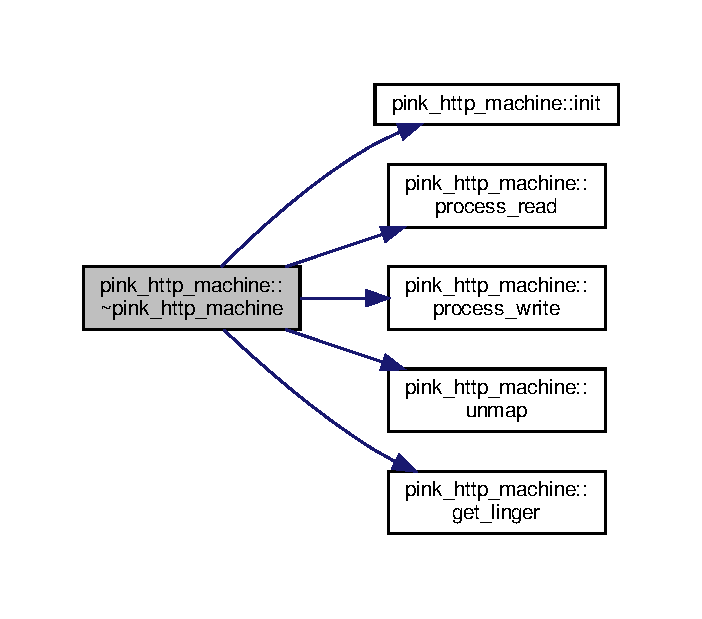
\includegraphics[width=337pt]{classpink__http__machine_a38d1d6228955fc97c752d330d4c126c2_cgraph}
\end{center}
\end{figure}


\subsection{Member Function Documentation}
\mbox{\Hypertarget{classpink__http__machine_a01dcf59a537c21d5a4a92c1c25fbf3ab}\label{classpink__http__machine_a01dcf59a537c21d5a4a92c1c25fbf3ab}} 
\index{pink\+\_\+http\+\_\+machine@{pink\+\_\+http\+\_\+machine}!get\+\_\+linger@{get\+\_\+linger}}
\index{get\+\_\+linger@{get\+\_\+linger}!pink\+\_\+http\+\_\+machine@{pink\+\_\+http\+\_\+machine}}
\subsubsection{\texorpdfstring{get\+\_\+linger()}{get\_linger()}}
{\footnotesize\ttfamily bool pink\+\_\+http\+\_\+machine\+::get\+\_\+linger (\begin{DoxyParamCaption}{ }\end{DoxyParamCaption})}



Definition at line 515 of file pink\+\_\+http\+\_\+machine.\+cpp.

Here is the caller graph for this function\+:
\nopagebreak
\begin{figure}[H]
\begin{center}
\leavevmode
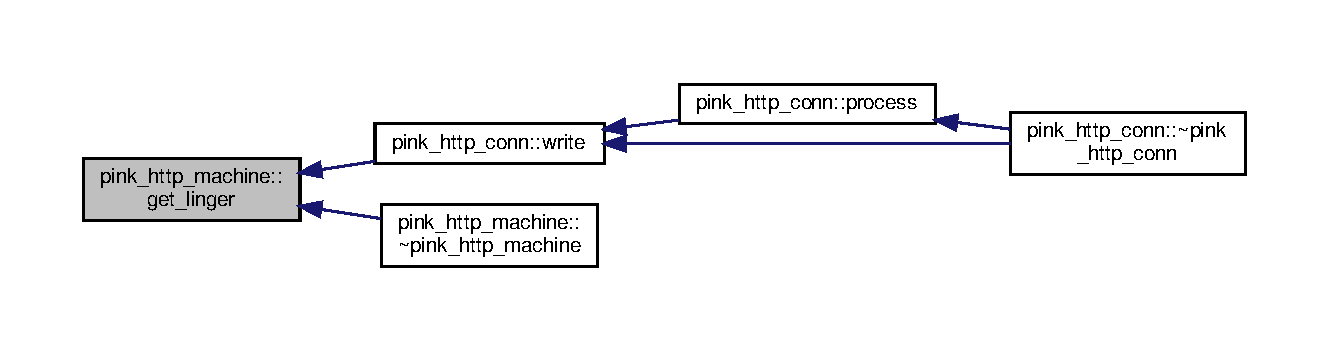
\includegraphics[width=350pt]{classpink__http__machine_a01dcf59a537c21d5a4a92c1c25fbf3ab_icgraph}
\end{center}
\end{figure}
\mbox{\Hypertarget{classpink__http__machine_a32b0ee47de1b90467d17194fa83b4eb0}\label{classpink__http__machine_a32b0ee47de1b90467d17194fa83b4eb0}} 
\index{pink\+\_\+http\+\_\+machine@{pink\+\_\+http\+\_\+machine}!init@{init}}
\index{init@{init}!pink\+\_\+http\+\_\+machine@{pink\+\_\+http\+\_\+machine}}
\subsubsection{\texorpdfstring{init()}{init()}}
{\footnotesize\ttfamily void pink\+\_\+http\+\_\+machine\+::init (\begin{DoxyParamCaption}\item[{char $\ast$}]{read\+\_\+buf,  }\item[{char $\ast$}]{write\+\_\+buf,  }\item[{int $\ast$}]{read\+\_\+idx,  }\item[{int $\ast$}]{write\+\_\+idx,  }\item[{const int}]{read\+\_\+buf\+\_\+size,  }\item[{const int}]{write\+\_\+buf\+\_\+size }\end{DoxyParamCaption})}



Definition at line 63 of file pink\+\_\+http\+\_\+machine.\+cpp.

Here is the caller graph for this function\+:
\nopagebreak
\begin{figure}[H]
\begin{center}
\leavevmode
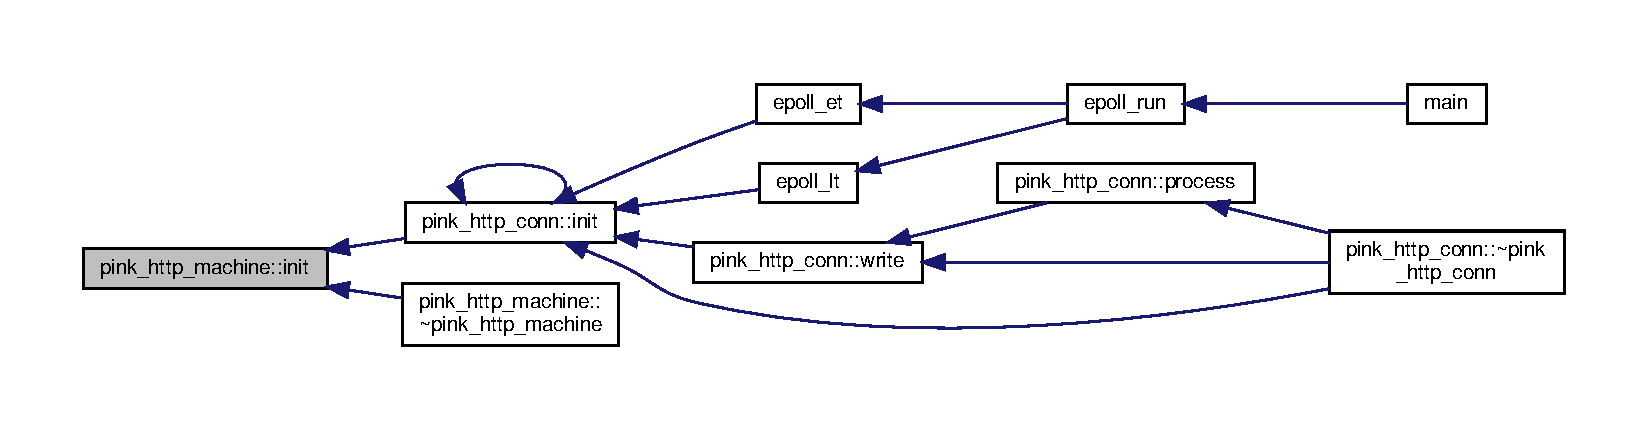
\includegraphics[width=350pt]{classpink__http__machine_a32b0ee47de1b90467d17194fa83b4eb0_icgraph}
\end{center}
\end{figure}
\mbox{\Hypertarget{classpink__http__machine_ad6d404392628f4b2c94a4b30fefb62f8}\label{classpink__http__machine_ad6d404392628f4b2c94a4b30fefb62f8}} 
\index{pink\+\_\+http\+\_\+machine@{pink\+\_\+http\+\_\+machine}!mime\+\_\+map\+\_\+init@{mime\+\_\+map\+\_\+init}}
\index{mime\+\_\+map\+\_\+init@{mime\+\_\+map\+\_\+init}!pink\+\_\+http\+\_\+machine@{pink\+\_\+http\+\_\+machine}}
\subsubsection{\texorpdfstring{mime\+\_\+map\+\_\+init()}{mime\_map\_init()}}
{\footnotesize\ttfamily std\+::unordered\+\_\+map$<$ string, string $>$ pink\+\_\+http\+\_\+machine\+::mime\+\_\+map\+\_\+init (\begin{DoxyParamCaption}{ }\end{DoxyParamCaption})\hspace{0.3cm}{\ttfamily [static]}}



Definition at line 26 of file pink\+\_\+http\+\_\+machine.\+cpp.

\mbox{\Hypertarget{classpink__http__machine_a7c937bd8da6bdfbf4894e6af9a712d60}\label{classpink__http__machine_a7c937bd8da6bdfbf4894e6af9a712d60}} 
\index{pink\+\_\+http\+\_\+machine@{pink\+\_\+http\+\_\+machine}!process\+\_\+read@{process\+\_\+read}}
\index{process\+\_\+read@{process\+\_\+read}!pink\+\_\+http\+\_\+machine@{pink\+\_\+http\+\_\+machine}}
\subsubsection{\texorpdfstring{process\+\_\+read()}{process\_read()}}
{\footnotesize\ttfamily \hyperlink{classpink__http__machine_afb1e590cd61676c2f8859c4e01e5b150}{pink\+\_\+http\+\_\+machine\+::\+H\+T\+T\+P\+\_\+\+C\+O\+DE} pink\+\_\+http\+\_\+machine\+::process\+\_\+read (\begin{DoxyParamCaption}{ }\end{DoxyParamCaption})}



Definition at line 101 of file pink\+\_\+http\+\_\+machine.\+cpp.

Here is the caller graph for this function\+:
\nopagebreak
\begin{figure}[H]
\begin{center}
\leavevmode
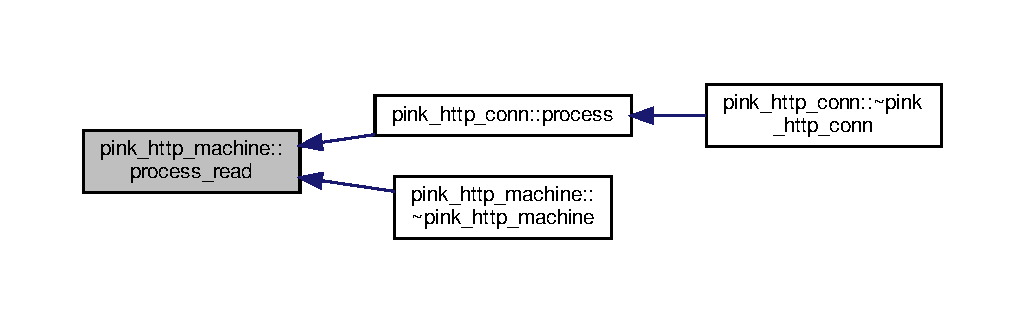
\includegraphics[width=350pt]{classpink__http__machine_a7c937bd8da6bdfbf4894e6af9a712d60_icgraph}
\end{center}
\end{figure}
\mbox{\Hypertarget{classpink__http__machine_a7144e4279cd09ab8ce56873bd3906f24}\label{classpink__http__machine_a7144e4279cd09ab8ce56873bd3906f24}} 
\index{pink\+\_\+http\+\_\+machine@{pink\+\_\+http\+\_\+machine}!process\+\_\+write@{process\+\_\+write}}
\index{process\+\_\+write@{process\+\_\+write}!pink\+\_\+http\+\_\+machine@{pink\+\_\+http\+\_\+machine}}
\subsubsection{\texorpdfstring{process\+\_\+write()}{process\_write()}}
{\footnotesize\ttfamily bool pink\+\_\+http\+\_\+machine\+::process\+\_\+write (\begin{DoxyParamCaption}\item[{\hyperlink{classpink__http__machine_afb1e590cd61676c2f8859c4e01e5b150}{H\+T\+T\+P\+\_\+\+C\+O\+DE}}]{ret,  }\item[{struct iovec $\ast$}]{iv,  }\item[{int \&}]{iv\+\_\+count }\end{DoxyParamCaption})}



Definition at line 394 of file pink\+\_\+http\+\_\+machine.\+cpp.

Here is the caller graph for this function\+:
\nopagebreak
\begin{figure}[H]
\begin{center}
\leavevmode
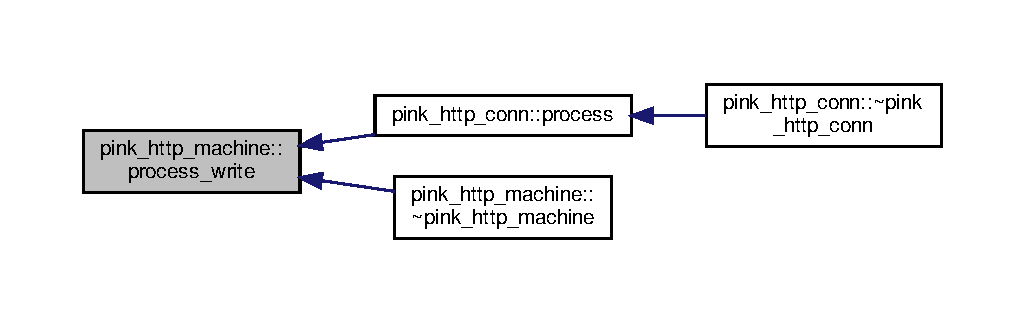
\includegraphics[width=350pt]{classpink__http__machine_a7144e4279cd09ab8ce56873bd3906f24_icgraph}
\end{center}
\end{figure}
\mbox{\Hypertarget{classpink__http__machine_a26debab8c361df5c79966f11e2b2dd17}\label{classpink__http__machine_a26debab8c361df5c79966f11e2b2dd17}} 
\index{pink\+\_\+http\+\_\+machine@{pink\+\_\+http\+\_\+machine}!unmap@{unmap}}
\index{unmap@{unmap}!pink\+\_\+http\+\_\+machine@{pink\+\_\+http\+\_\+machine}}
\subsubsection{\texorpdfstring{unmap()}{unmap()}}
{\footnotesize\ttfamily void pink\+\_\+http\+\_\+machine\+::unmap (\begin{DoxyParamCaption}{ }\end{DoxyParamCaption})}



Definition at line 519 of file pink\+\_\+http\+\_\+machine.\+cpp.

Here is the caller graph for this function\+:
\nopagebreak
\begin{figure}[H]
\begin{center}
\leavevmode
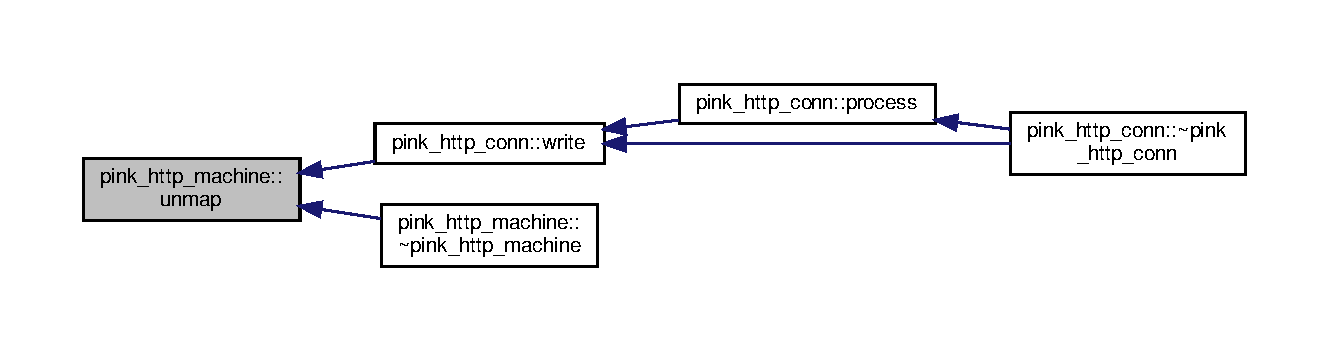
\includegraphics[width=350pt]{classpink__http__machine_a26debab8c361df5c79966f11e2b2dd17_icgraph}
\end{center}
\end{figure}


\subsection{Member Data Documentation}
\mbox{\Hypertarget{classpink__http__machine_a33993ee83910b37ae5672c6e6c94cac3}\label{classpink__http__machine_a33993ee83910b37ae5672c6e6c94cac3}} 
\index{pink\+\_\+http\+\_\+machine@{pink\+\_\+http\+\_\+machine}!F\+I\+L\+E\+N\+A\+M\+E\+\_\+\+L\+EN@{F\+I\+L\+E\+N\+A\+M\+E\+\_\+\+L\+EN}}
\index{F\+I\+L\+E\+N\+A\+M\+E\+\_\+\+L\+EN@{F\+I\+L\+E\+N\+A\+M\+E\+\_\+\+L\+EN}!pink\+\_\+http\+\_\+machine@{pink\+\_\+http\+\_\+machine}}
\subsubsection{\texorpdfstring{F\+I\+L\+E\+N\+A\+M\+E\+\_\+\+L\+EN}{FILENAME\_LEN}}
{\footnotesize\ttfamily constexpr int pink\+\_\+http\+\_\+machine\+::\+F\+I\+L\+E\+N\+A\+M\+E\+\_\+\+L\+EN = 1024\hspace{0.3cm}{\ttfamily [static]}}



Definition at line 87 of file pink\+\_\+http\+\_\+machine.\+h.

\mbox{\Hypertarget{classpink__http__machine_a4373363c5bd675e182f502d300157aa9}\label{classpink__http__machine_a4373363c5bd675e182f502d300157aa9}} 
\index{pink\+\_\+http\+\_\+machine@{pink\+\_\+http\+\_\+machine}!mime\+\_\+type@{mime\+\_\+type}}
\index{mime\+\_\+type@{mime\+\_\+type}!pink\+\_\+http\+\_\+machine@{pink\+\_\+http\+\_\+machine}}
\subsubsection{\texorpdfstring{mime\+\_\+type}{mime\_type}}
{\footnotesize\ttfamily std\+::unordered\+\_\+map$<$ string, string $>$ pink\+\_\+http\+\_\+machine\+::mime\+\_\+type\hspace{0.3cm}{\ttfamily [static]}}

{\bfseries Initial value\+:}
\begin{DoxyCode}
= 
                                \hyperlink{classpink__http__machine_ad6d404392628f4b2c94a4b30fefb62f8}{pink\_http\_machine::mime\_map\_init}()
\end{DoxyCode}


Definition at line 89 of file pink\+\_\+http\+\_\+machine.\+h.



The documentation for this class was generated from the following files\+:\begin{DoxyCompactItemize}
\item 
\hyperlink{pink__http__machine_8h}{pink\+\_\+http\+\_\+machine.\+h}\item 
\hyperlink{pink__http__machine_8cpp}{pink\+\_\+http\+\_\+machine.\+cpp}\end{DoxyCompactItemize}

\hypertarget{classpink__mem__pool}{}\section{pink\+\_\+mem\+\_\+pool Class Reference}
\label{classpink__mem__pool}\index{pink\+\_\+mem\+\_\+pool@{pink\+\_\+mem\+\_\+pool}}


{\ttfamily \#include $<$pink\+\_\+mem\+\_\+pool.\+h$>$}

\subsection*{Static Public Member Functions}
\begin{DoxyCompactItemize}
\item 
static void $\ast$ \hyperlink{classpink__mem__pool_a4d49dea3bf3b915e30f105e7027ef07d}{allocate} (size\+\_\+t n)
\item 
static void $\ast$ \hyperlink{classpink__mem__pool_a4558b3b63009b917441d763619eeb4f4}{deallocate} (void $\ast$p, size\+\_\+t n)
\end{DoxyCompactItemize}


\subsection{Detailed Description}


Definition at line 6 of file pink\+\_\+mem\+\_\+pool.\+h.



\subsection{Member Function Documentation}
\mbox{\Hypertarget{classpink__mem__pool_a4d49dea3bf3b915e30f105e7027ef07d}\label{classpink__mem__pool_a4d49dea3bf3b915e30f105e7027ef07d}} 
\index{pink\+\_\+mem\+\_\+pool@{pink\+\_\+mem\+\_\+pool}!allocate@{allocate}}
\index{allocate@{allocate}!pink\+\_\+mem\+\_\+pool@{pink\+\_\+mem\+\_\+pool}}
\subsubsection{\texorpdfstring{allocate()}{allocate()}}
{\footnotesize\ttfamily void $\ast$ pink\+\_\+mem\+\_\+pool\+::allocate (\begin{DoxyParamCaption}\item[{size\+\_\+t}]{n }\end{DoxyParamCaption})\hspace{0.3cm}{\ttfamily [static]}}



Definition at line 42 of file pink\+\_\+mem\+\_\+pool.\+h.

\mbox{\Hypertarget{classpink__mem__pool_a4558b3b63009b917441d763619eeb4f4}\label{classpink__mem__pool_a4558b3b63009b917441d763619eeb4f4}} 
\index{pink\+\_\+mem\+\_\+pool@{pink\+\_\+mem\+\_\+pool}!deallocate@{deallocate}}
\index{deallocate@{deallocate}!pink\+\_\+mem\+\_\+pool@{pink\+\_\+mem\+\_\+pool}}
\subsubsection{\texorpdfstring{deallocate()}{deallocate()}}
{\footnotesize\ttfamily void $\ast$ pink\+\_\+mem\+\_\+pool\+::deallocate (\begin{DoxyParamCaption}\item[{void $\ast$}]{p,  }\item[{size\+\_\+t}]{n }\end{DoxyParamCaption})\hspace{0.3cm}{\ttfamily [static]}}



Definition at line 46 of file pink\+\_\+mem\+\_\+pool.\+h.



The documentation for this class was generated from the following file\+:\begin{DoxyCompactItemize}
\item 
\hyperlink{pink__mem__pool_8h}{pink\+\_\+mem\+\_\+pool.\+h}\end{DoxyCompactItemize}

\hypertarget{classpink__threadpool}{}\section{pink\+\_\+threadpool$<$ T $>$ Class Template Reference}
\label{classpink__threadpool}\index{pink\+\_\+threadpool$<$ T $>$@{pink\+\_\+threadpool$<$ T $>$}}
\subsection*{Public Member Functions}
\begin{DoxyCompactItemize}
\item 
\mbox{\Hypertarget{classpink__threadpool_a75dcfa67e83f32078d65f263cae5b118}\label{classpink__threadpool_a75dcfa67e83f32078d65f263cae5b118}} 
{\bfseries pink\+\_\+threadpool} (int thread\+\_\+number=8, int max\+\_\+requests=100000)
\item 
\mbox{\Hypertarget{classpink__threadpool_ae4bead5c98203b97c3caeae43296d295}\label{classpink__threadpool_ae4bead5c98203b97c3caeae43296d295}} 
bool {\bfseries append} (T $\ast$request, int flag)
\end{DoxyCompactItemize}


The documentation for this class was generated from the following file\+:\begin{DoxyCompactItemize}
\item 
pink\+\_\+thread\+\_\+pool.\+h\end{DoxyCompactItemize}

\hypertarget{classpink__time__heap}{}\section{pink\+\_\+time\+\_\+heap Class Reference}
\label{classpink__time__heap}\index{pink\+\_\+time\+\_\+heap@{pink\+\_\+time\+\_\+heap}}


{\ttfamily \#include $<$pink\+\_\+epoll.\+h$>$}

\subsection*{Public Member Functions}
\begin{DoxyCompactItemize}
\item 
\hyperlink{classpink__time__heap_a72c02a943378fc5573ba55c614fc4b8d}{pink\+\_\+time\+\_\+heap} ()=default
\item 
\hyperlink{classpink__time__heap_a45279534f708648c2f51d166fe0a376a}{pink\+\_\+time\+\_\+heap} (int init\+\_\+cap=1024)
\item 
\hyperlink{classpink__time__heap_a6aed9951c6c206e7752fa304d8fec612}{$\sim$pink\+\_\+time\+\_\+heap} ()
\item 
void \hyperlink{classpink__time__heap_aa74cc12fe4a94acbe75b70a3962a862f}{push} (\hyperlink{classconn__timer}{conn\+\_\+timer} $\ast$t)
\item 
void \hyperlink{classpink__time__heap_a331d1f993efc7bd50f8e6d10e5f1c6ee}{cancel} (\hyperlink{classconn__timer}{conn\+\_\+timer} $\ast$t)
\item 
\hyperlink{classconn__timer}{conn\+\_\+timer} $\ast$ \hyperlink{classpink__time__heap_ac0932b13390241373290a321ecf16600}{top} () const
\item 
void \hyperlink{classpink__time__heap_a5642ee3340cdee7983ed63770e7109d1}{pop} ()
\item 
void \hyperlink{classpink__time__heap_a9193dc948c6bb00005bf6639f2169b57}{tick} ()
\item 
bool \hyperlink{classpink__time__heap_ade64cf32193747380cb57c5709e28383}{empty} () const
\end{DoxyCompactItemize}


\subsection{Detailed Description}


Definition at line 24 of file pink\+\_\+epoll.\+h.



\subsection{Constructor \& Destructor Documentation}
\mbox{\Hypertarget{classpink__time__heap_a72c02a943378fc5573ba55c614fc4b8d}\label{classpink__time__heap_a72c02a943378fc5573ba55c614fc4b8d}} 
\index{pink\+\_\+time\+\_\+heap@{pink\+\_\+time\+\_\+heap}!pink\+\_\+time\+\_\+heap@{pink\+\_\+time\+\_\+heap}}
\index{pink\+\_\+time\+\_\+heap@{pink\+\_\+time\+\_\+heap}!pink\+\_\+time\+\_\+heap@{pink\+\_\+time\+\_\+heap}}
\subsubsection{\texorpdfstring{pink\+\_\+time\+\_\+heap()}{pink\_time\_heap()}\hspace{0.1cm}{\footnotesize\ttfamily [1/2]}}
{\footnotesize\ttfamily pink\+\_\+time\+\_\+heap\+::pink\+\_\+time\+\_\+heap (\begin{DoxyParamCaption}{ }\end{DoxyParamCaption})\hspace{0.3cm}{\ttfamily [default]}}

\mbox{\Hypertarget{classpink__time__heap_a45279534f708648c2f51d166fe0a376a}\label{classpink__time__heap_a45279534f708648c2f51d166fe0a376a}} 
\index{pink\+\_\+time\+\_\+heap@{pink\+\_\+time\+\_\+heap}!pink\+\_\+time\+\_\+heap@{pink\+\_\+time\+\_\+heap}}
\index{pink\+\_\+time\+\_\+heap@{pink\+\_\+time\+\_\+heap}!pink\+\_\+time\+\_\+heap@{pink\+\_\+time\+\_\+heap}}
\subsubsection{\texorpdfstring{pink\+\_\+time\+\_\+heap()}{pink\_time\_heap()}\hspace{0.1cm}{\footnotesize\ttfamily [2/2]}}
{\footnotesize\ttfamily pink\+\_\+time\+\_\+heap\+::pink\+\_\+time\+\_\+heap (\begin{DoxyParamCaption}\item[{int}]{init\+\_\+cap = {\ttfamily 1024} }\end{DoxyParamCaption})}



Definition at line 192 of file pink\+\_\+epoll.\+cpp.

\mbox{\Hypertarget{classpink__time__heap_a6aed9951c6c206e7752fa304d8fec612}\label{classpink__time__heap_a6aed9951c6c206e7752fa304d8fec612}} 
\index{pink\+\_\+time\+\_\+heap@{pink\+\_\+time\+\_\+heap}!````~pink\+\_\+time\+\_\+heap@{$\sim$pink\+\_\+time\+\_\+heap}}
\index{````~pink\+\_\+time\+\_\+heap@{$\sim$pink\+\_\+time\+\_\+heap}!pink\+\_\+time\+\_\+heap@{pink\+\_\+time\+\_\+heap}}
\subsubsection{\texorpdfstring{$\sim$pink\+\_\+time\+\_\+heap()}{~pink\_time\_heap()}}
{\footnotesize\ttfamily pink\+\_\+time\+\_\+heap\+::$\sim$pink\+\_\+time\+\_\+heap (\begin{DoxyParamCaption}{ }\end{DoxyParamCaption})}



Definition at line 202 of file pink\+\_\+epoll.\+cpp.



\subsection{Member Function Documentation}
\mbox{\Hypertarget{classpink__time__heap_a331d1f993efc7bd50f8e6d10e5f1c6ee}\label{classpink__time__heap_a331d1f993efc7bd50f8e6d10e5f1c6ee}} 
\index{pink\+\_\+time\+\_\+heap@{pink\+\_\+time\+\_\+heap}!cancel@{cancel}}
\index{cancel@{cancel}!pink\+\_\+time\+\_\+heap@{pink\+\_\+time\+\_\+heap}}
\subsubsection{\texorpdfstring{cancel()}{cancel()}}
{\footnotesize\ttfamily void pink\+\_\+time\+\_\+heap\+::cancel (\begin{DoxyParamCaption}\item[{\hyperlink{classconn__timer}{conn\+\_\+timer} $\ast$}]{t }\end{DoxyParamCaption})}



Definition at line 222 of file pink\+\_\+epoll.\+cpp.

Here is the call graph for this function\+:\nopagebreak
\begin{figure}[H]
\begin{center}
\leavevmode
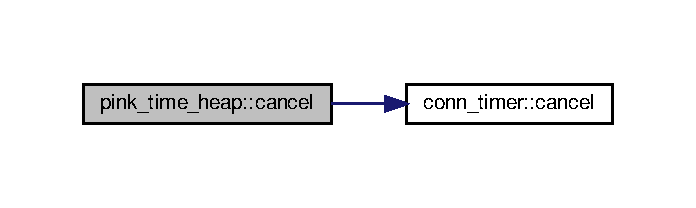
\includegraphics[width=334pt]{classpink__time__heap_a331d1f993efc7bd50f8e6d10e5f1c6ee_cgraph}
\end{center}
\end{figure}
\mbox{\Hypertarget{classpink__time__heap_ade64cf32193747380cb57c5709e28383}\label{classpink__time__heap_ade64cf32193747380cb57c5709e28383}} 
\index{pink\+\_\+time\+\_\+heap@{pink\+\_\+time\+\_\+heap}!empty@{empty}}
\index{empty@{empty}!pink\+\_\+time\+\_\+heap@{pink\+\_\+time\+\_\+heap}}
\subsubsection{\texorpdfstring{empty()}{empty()}}
{\footnotesize\ttfamily bool pink\+\_\+time\+\_\+heap\+::empty (\begin{DoxyParamCaption}{ }\end{DoxyParamCaption}) const}



Definition at line 258 of file pink\+\_\+epoll.\+cpp.

Here is the caller graph for this function\+:\nopagebreak
\begin{figure}[H]
\begin{center}
\leavevmode
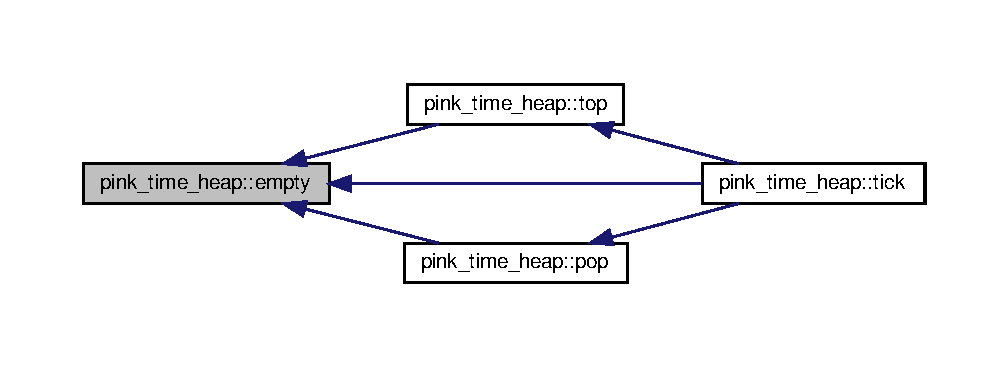
\includegraphics[width=350pt]{classpink__time__heap_ade64cf32193747380cb57c5709e28383_icgraph}
\end{center}
\end{figure}
\mbox{\Hypertarget{classpink__time__heap_a5642ee3340cdee7983ed63770e7109d1}\label{classpink__time__heap_a5642ee3340cdee7983ed63770e7109d1}} 
\index{pink\+\_\+time\+\_\+heap@{pink\+\_\+time\+\_\+heap}!pop@{pop}}
\index{pop@{pop}!pink\+\_\+time\+\_\+heap@{pink\+\_\+time\+\_\+heap}}
\subsubsection{\texorpdfstring{pop()}{pop()}}
{\footnotesize\ttfamily void pink\+\_\+time\+\_\+heap\+::pop (\begin{DoxyParamCaption}{ }\end{DoxyParamCaption})}



Definition at line 235 of file pink\+\_\+epoll.\+cpp.

Here is the call graph for this function\+:\nopagebreak
\begin{figure}[H]
\begin{center}
\leavevmode
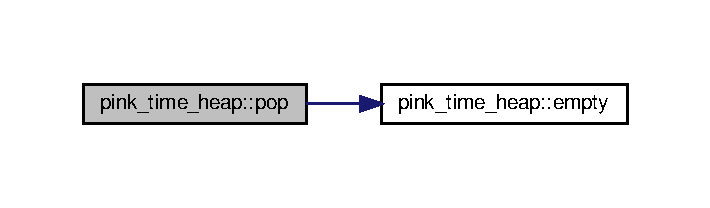
\includegraphics[width=341pt]{classpink__time__heap_a5642ee3340cdee7983ed63770e7109d1_cgraph}
\end{center}
\end{figure}
Here is the caller graph for this function\+:\nopagebreak
\begin{figure}[H]
\begin{center}
\leavevmode
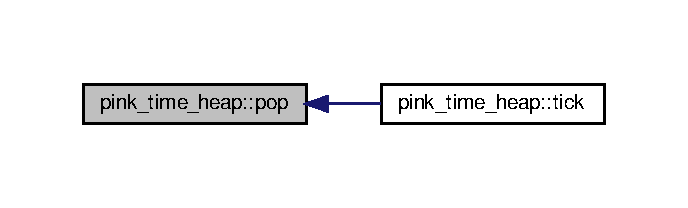
\includegraphics[width=330pt]{classpink__time__heap_a5642ee3340cdee7983ed63770e7109d1_icgraph}
\end{center}
\end{figure}
\mbox{\Hypertarget{classpink__time__heap_aa74cc12fe4a94acbe75b70a3962a862f}\label{classpink__time__heap_aa74cc12fe4a94acbe75b70a3962a862f}} 
\index{pink\+\_\+time\+\_\+heap@{pink\+\_\+time\+\_\+heap}!push@{push}}
\index{push@{push}!pink\+\_\+time\+\_\+heap@{pink\+\_\+time\+\_\+heap}}
\subsubsection{\texorpdfstring{push()}{push()}}
{\footnotesize\ttfamily void pink\+\_\+time\+\_\+heap\+::push (\begin{DoxyParamCaption}\item[{\hyperlink{classconn__timer}{conn\+\_\+timer} $\ast$}]{t }\end{DoxyParamCaption})}



Definition at line 207 of file pink\+\_\+epoll.\+cpp.

\mbox{\Hypertarget{classpink__time__heap_a9193dc948c6bb00005bf6639f2169b57}\label{classpink__time__heap_a9193dc948c6bb00005bf6639f2169b57}} 
\index{pink\+\_\+time\+\_\+heap@{pink\+\_\+time\+\_\+heap}!tick@{tick}}
\index{tick@{tick}!pink\+\_\+time\+\_\+heap@{pink\+\_\+time\+\_\+heap}}
\subsubsection{\texorpdfstring{tick()}{tick()}}
{\footnotesize\ttfamily void pink\+\_\+time\+\_\+heap\+::tick (\begin{DoxyParamCaption}{ }\end{DoxyParamCaption})}



Definition at line 245 of file pink\+\_\+epoll.\+cpp.

Here is the call graph for this function\+:\nopagebreak
\begin{figure}[H]
\begin{center}
\leavevmode
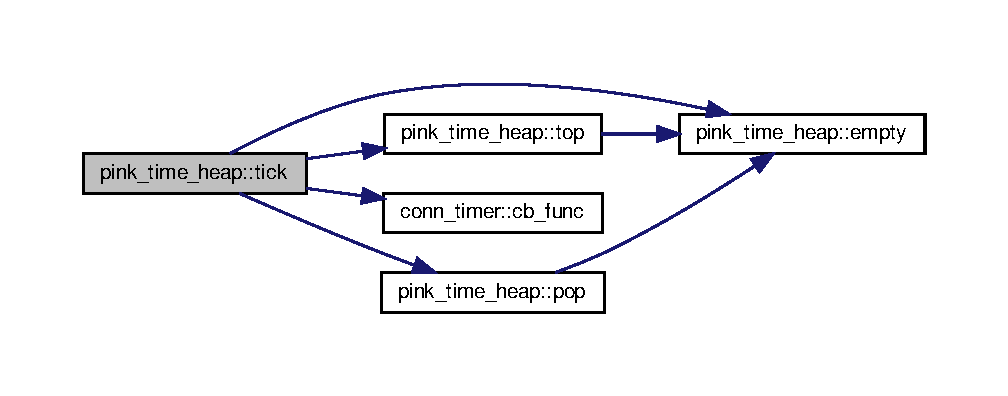
\includegraphics[width=350pt]{classpink__time__heap_a9193dc948c6bb00005bf6639f2169b57_cgraph}
\end{center}
\end{figure}
\mbox{\Hypertarget{classpink__time__heap_ac0932b13390241373290a321ecf16600}\label{classpink__time__heap_ac0932b13390241373290a321ecf16600}} 
\index{pink\+\_\+time\+\_\+heap@{pink\+\_\+time\+\_\+heap}!top@{top}}
\index{top@{top}!pink\+\_\+time\+\_\+heap@{pink\+\_\+time\+\_\+heap}}
\subsubsection{\texorpdfstring{top()}{top()}}
{\footnotesize\ttfamily \hyperlink{classconn__timer}{conn\+\_\+timer} $\ast$ pink\+\_\+time\+\_\+heap\+::top (\begin{DoxyParamCaption}{ }\end{DoxyParamCaption}) const}



Definition at line 229 of file pink\+\_\+epoll.\+cpp.

Here is the call graph for this function\+:\nopagebreak
\begin{figure}[H]
\begin{center}
\leavevmode
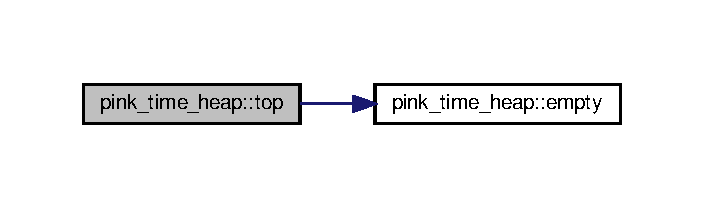
\includegraphics[width=338pt]{classpink__time__heap_ac0932b13390241373290a321ecf16600_cgraph}
\end{center}
\end{figure}
Here is the caller graph for this function\+:\nopagebreak
\begin{figure}[H]
\begin{center}
\leavevmode
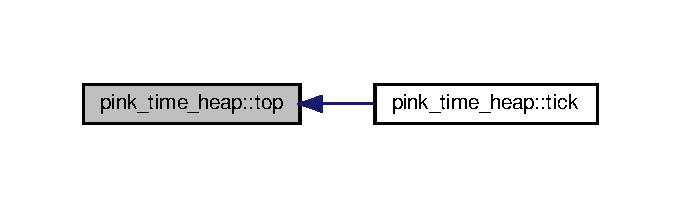
\includegraphics[width=327pt]{classpink__time__heap_ac0932b13390241373290a321ecf16600_icgraph}
\end{center}
\end{figure}


The documentation for this class was generated from the following files\+:\begin{DoxyCompactItemize}
\item 
\hyperlink{pink__epoll_8h}{pink\+\_\+epoll.\+h}\item 
\hyperlink{pink__epoll_8cpp}{pink\+\_\+epoll.\+cpp}\end{DoxyCompactItemize}

\hypertarget{classsem}{}\section{sem Class Reference}
\label{classsem}\index{sem@{sem}}


{\ttfamily \#include $<$I\+P\+C\+\_\+tool.\+h$>$}

\subsection*{Public Member Functions}
\begin{DoxyCompactItemize}
\item 
\hyperlink{classsem_afc49c4ced0a9986bf4b6da4f10d45a4b}{sem} ()
\item 
\hyperlink{classsem_a8e5210bd3255149e3a56d69dbc0cba60}{$\sim$sem} ()
\item 
bool \hyperlink{classsem_a0195e3b2273cb8d2c814778b0521e847}{wait} ()
\item 
bool \hyperlink{classsem_a258d9983b317cba4b528f6204545f849}{post} ()
\end{DoxyCompactItemize}


\subsection{Detailed Description}


Definition at line 10 of file I\+P\+C\+\_\+tool.\+h.



\subsection{Constructor \& Destructor Documentation}
\mbox{\Hypertarget{classsem_afc49c4ced0a9986bf4b6da4f10d45a4b}\label{classsem_afc49c4ced0a9986bf4b6da4f10d45a4b}} 
\index{sem@{sem}!sem@{sem}}
\index{sem@{sem}!sem@{sem}}
\subsubsection{\texorpdfstring{sem()}{sem()}}
{\footnotesize\ttfamily sem\+::sem (\begin{DoxyParamCaption}{ }\end{DoxyParamCaption})\hspace{0.3cm}{\ttfamily [inline]}}



Definition at line 12 of file I\+P\+C\+\_\+tool.\+h.

\mbox{\Hypertarget{classsem_a8e5210bd3255149e3a56d69dbc0cba60}\label{classsem_a8e5210bd3255149e3a56d69dbc0cba60}} 
\index{sem@{sem}!````~sem@{$\sim$sem}}
\index{````~sem@{$\sim$sem}!sem@{sem}}
\subsubsection{\texorpdfstring{$\sim$sem()}{~sem()}}
{\footnotesize\ttfamily sem\+::$\sim$sem (\begin{DoxyParamCaption}{ }\end{DoxyParamCaption})\hspace{0.3cm}{\ttfamily [inline]}}



Definition at line 17 of file I\+P\+C\+\_\+tool.\+h.



\subsection{Member Function Documentation}
\mbox{\Hypertarget{classsem_a258d9983b317cba4b528f6204545f849}\label{classsem_a258d9983b317cba4b528f6204545f849}} 
\index{sem@{sem}!post@{post}}
\index{post@{post}!sem@{sem}}
\subsubsection{\texorpdfstring{post()}{post()}}
{\footnotesize\ttfamily bool sem\+::post (\begin{DoxyParamCaption}{ }\end{DoxyParamCaption})\hspace{0.3cm}{\ttfamily [inline]}}



Definition at line 23 of file I\+P\+C\+\_\+tool.\+h.

Here is the caller graph for this function\+:\nopagebreak
\begin{figure}[H]
\begin{center}
\leavevmode
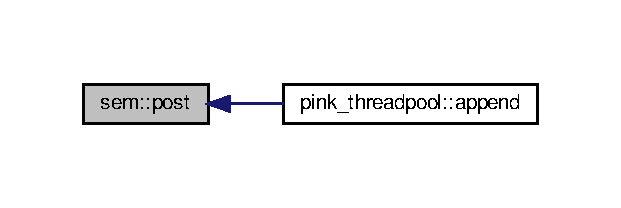
\includegraphics[width=298pt]{classsem_a258d9983b317cba4b528f6204545f849_icgraph}
\end{center}
\end{figure}
\mbox{\Hypertarget{classsem_a0195e3b2273cb8d2c814778b0521e847}\label{classsem_a0195e3b2273cb8d2c814778b0521e847}} 
\index{sem@{sem}!wait@{wait}}
\index{wait@{wait}!sem@{sem}}
\subsubsection{\texorpdfstring{wait()}{wait()}}
{\footnotesize\ttfamily bool sem\+::wait (\begin{DoxyParamCaption}{ }\end{DoxyParamCaption})\hspace{0.3cm}{\ttfamily [inline]}}



Definition at line 20 of file I\+P\+C\+\_\+tool.\+h.

Here is the caller graph for this function\+:\nopagebreak
\begin{figure}[H]
\begin{center}
\leavevmode
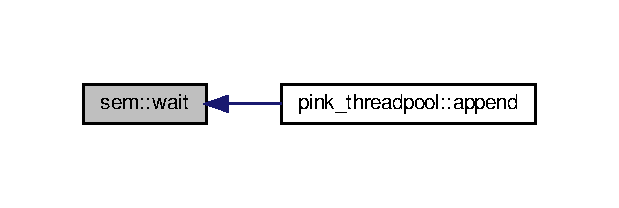
\includegraphics[width=297pt]{classsem_a0195e3b2273cb8d2c814778b0521e847_icgraph}
\end{center}
\end{figure}


The documentation for this class was generated from the following file\+:\begin{DoxyCompactItemize}
\item 
tools/\hyperlink{_i_p_c__tool_8h}{I\+P\+C\+\_\+tool.\+h}\end{DoxyCompactItemize}

\chapter{File Documentation}
\hypertarget{architecture_8md}{}\section{knowledge/architecture.md File Reference}
\label{architecture_8md}\index{knowledge/architecture.\+md@{knowledge/architecture.\+md}}

\hypertarget{basic_8md}{}\section{knowledge/basic.md File Reference}
\label{basic_8md}\index{knowledge/basic.\+md@{knowledge/basic.\+md}}

\hypertarget{evaluation_8md}{}\section{knowledge/evaluation.md File Reference}
\label{evaluation_8md}\index{knowledge/evaluation.\+md@{knowledge/evaluation.\+md}}

\hypertarget{problems_8md}{}\section{knowledge/problems.md File Reference}
\label{problems_8md}\index{knowledge/problems.\+md@{knowledge/problems.\+md}}

\hypertarget{knowledge_2_r_e_a_d_m_e_8md}{}\section{knowledge/\+R\+E\+A\+D\+ME.md File Reference}
\label{knowledge_2_r_e_a_d_m_e_8md}\index{knowledge/\+R\+E\+A\+D\+M\+E.\+md@{knowledge/\+R\+E\+A\+D\+M\+E.\+md}}

\hypertarget{_r_e_a_d_m_e_8md}{}\section{R\+E\+A\+D\+M\+E.\+md File Reference}
\label{_r_e_a_d_m_e_8md}\index{R\+E\+A\+D\+M\+E.\+md@{R\+E\+A\+D\+M\+E.\+md}}

\hypertarget{_xE6_x83_x8A_xE7_xBE_xA4_xE9_x97_xAE_xE9_xA2_x98_8md}{}\section{knowledge/惊群问题.md File Reference}
\label{_xE6_x83_x8A_xE7_xBE_xA4_xE9_x97_xAE_xE9_xA2_x98_8md}\index{knowledge/惊群问题.\+md@{knowledge/惊群问题.\+md}}

\hypertarget{main_8cpp}{}\section{main.\+cpp File Reference}
\label{main_8cpp}\index{main.\+cpp@{main.\+cpp}}
{\ttfamily \#include $<$iostream$>$}\newline
{\ttfamily \#include $<$vector$>$}\newline
{\ttfamily \#include $<$signal.\+h$>$}\newline
{\ttfamily \#include \char`\"{}pink\+\_\+epoll.\+h\char`\"{}}\newline
Include dependency graph for main.\+cpp\+:
\nopagebreak
\begin{figure}[H]
\begin{center}
\leavevmode
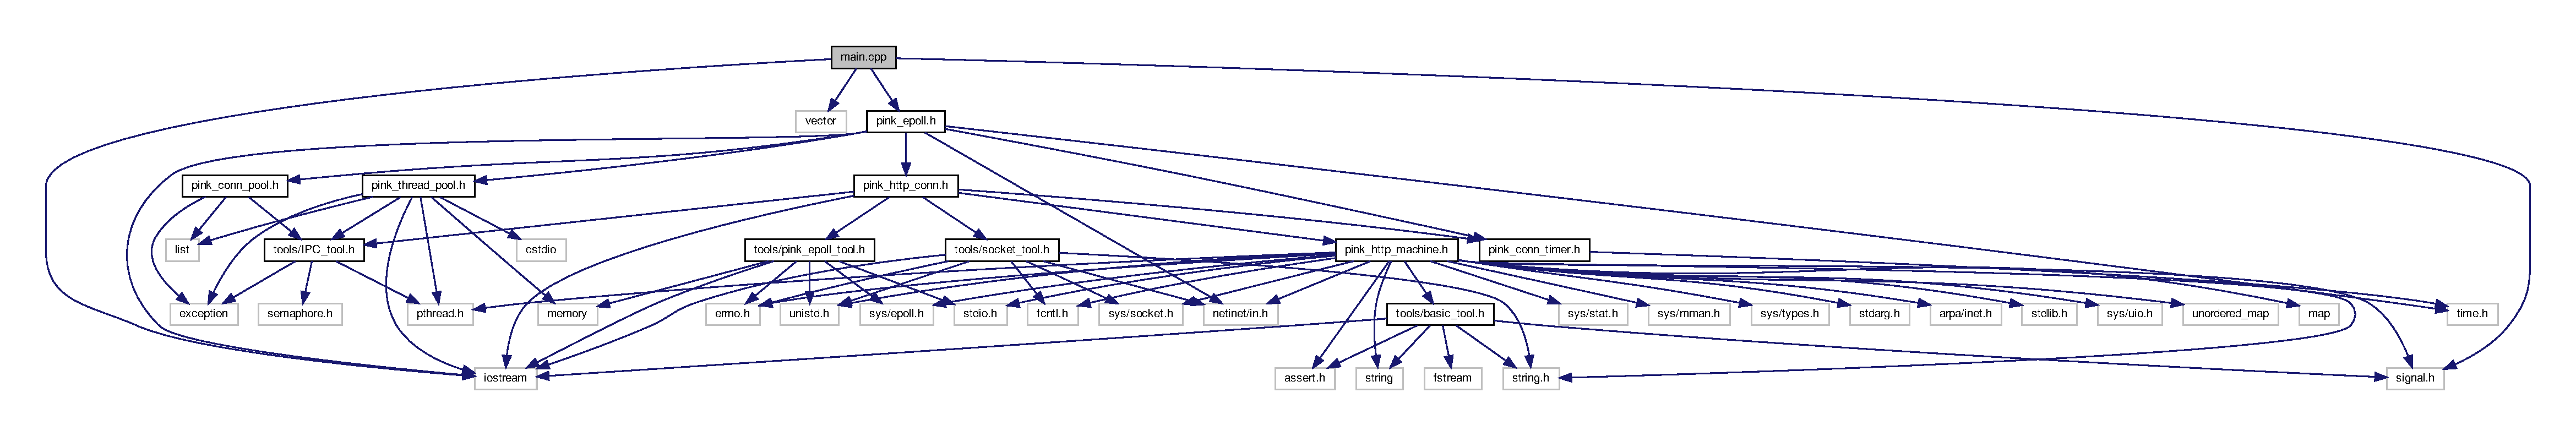
\includegraphics[width=350pt]{main_8cpp__incl}
\end{center}
\end{figure}
\subsection*{Functions}
\begin{DoxyCompactItemize}
\item 
int \hyperlink{main_8cpp_a0ddf1224851353fc92bfbff6f499fa97}{main} (int argc, char $\ast$argv\mbox{[}$\,$\mbox{]})
\end{DoxyCompactItemize}
\subsection*{Variables}
\begin{DoxyCompactItemize}
\item 
const char $\ast$ \hyperlink{main_8cpp_afe6c02e12089e94c4cb9f21860a08509}{conf\+\_\+file} = \char`\"{}pink\+\_\+conf.\+conf\char`\"{}
\item 
\hyperlink{basic__tool_8h_aa8adc7b5bceb1e76cda9b5ec5471159a}{conf\+\_\+t} \hyperlink{main_8cpp_a40e427255962e28d8913a56db7b748b8}{conf}
\end{DoxyCompactItemize}


\subsection{Function Documentation}
\mbox{\Hypertarget{main_8cpp_a0ddf1224851353fc92bfbff6f499fa97}\label{main_8cpp_a0ddf1224851353fc92bfbff6f499fa97}} 
\index{main.\+cpp@{main.\+cpp}!main@{main}}
\index{main@{main}!main.\+cpp@{main.\+cpp}}
\subsubsection{\texorpdfstring{main()}{main()}}
{\footnotesize\ttfamily int main (\begin{DoxyParamCaption}\item[{int}]{argc,  }\item[{char $\ast$}]{argv\mbox{[}$\,$\mbox{]} }\end{DoxyParamCaption})}



Definition at line 9 of file main.\+cpp.

Here is the call graph for this function\+:
\nopagebreak
\begin{figure}[H]
\begin{center}
\leavevmode
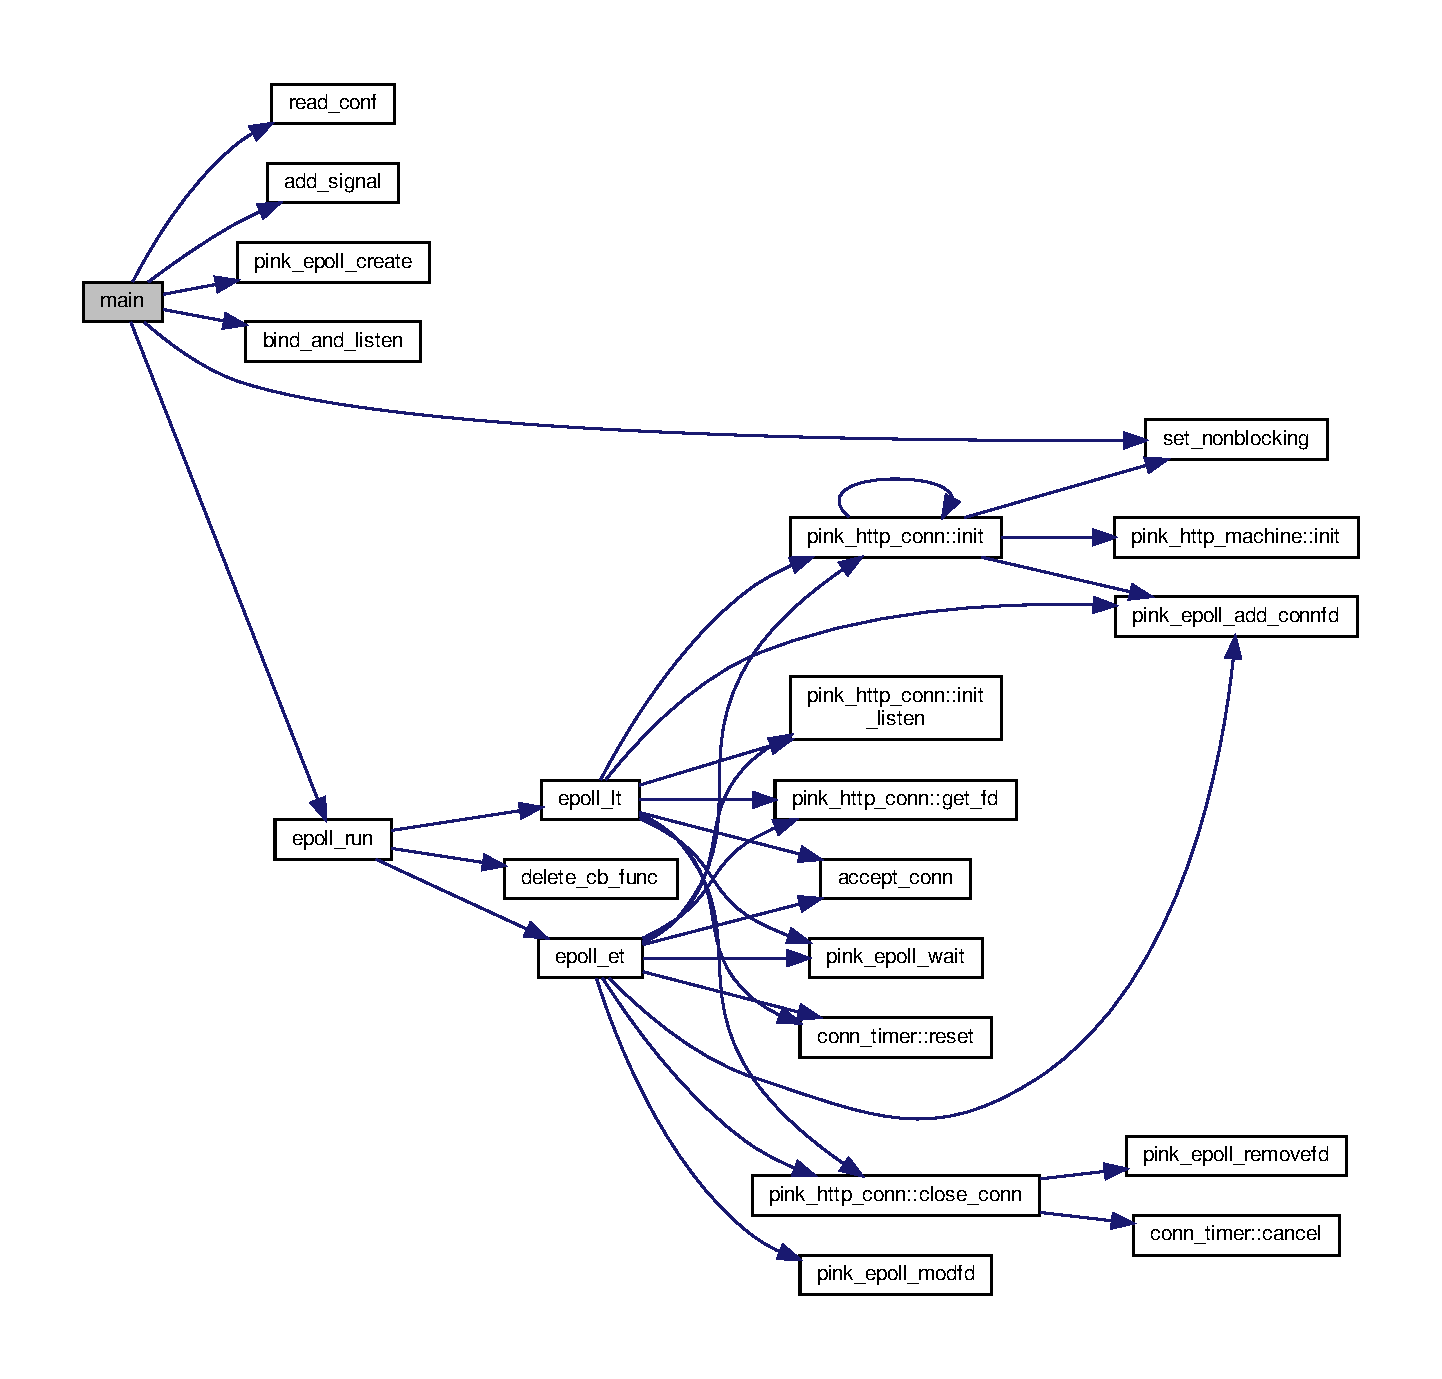
\includegraphics[width=350pt]{main_8cpp_a0ddf1224851353fc92bfbff6f499fa97_cgraph}
\end{center}
\end{figure}


\subsection{Variable Documentation}
\mbox{\Hypertarget{main_8cpp_a40e427255962e28d8913a56db7b748b8}\label{main_8cpp_a40e427255962e28d8913a56db7b748b8}} 
\index{main.\+cpp@{main.\+cpp}!conf@{conf}}
\index{conf@{conf}!main.\+cpp@{main.\+cpp}}
\subsubsection{\texorpdfstring{conf}{conf}}
{\footnotesize\ttfamily \hyperlink{basic__tool_8h_aa8adc7b5bceb1e76cda9b5ec5471159a}{conf\+\_\+t} conf}



Definition at line 7 of file main.\+cpp.

\mbox{\Hypertarget{main_8cpp_afe6c02e12089e94c4cb9f21860a08509}\label{main_8cpp_afe6c02e12089e94c4cb9f21860a08509}} 
\index{main.\+cpp@{main.\+cpp}!conf\+\_\+file@{conf\+\_\+file}}
\index{conf\+\_\+file@{conf\+\_\+file}!main.\+cpp@{main.\+cpp}}
\subsubsection{\texorpdfstring{conf\+\_\+file}{conf\_file}}
{\footnotesize\ttfamily const char$\ast$ conf\+\_\+file = \char`\"{}pink\+\_\+conf.\+conf\char`\"{}}



Definition at line 6 of file main.\+cpp.


\hypertarget{pink__conn__pool_8h}{}\section{pink\+\_\+conn\+\_\+pool.\+h File Reference}
\label{pink__conn__pool_8h}\index{pink\+\_\+conn\+\_\+pool.\+h@{pink\+\_\+conn\+\_\+pool.\+h}}
{\ttfamily \#include $<$list$>$}\newline
{\ttfamily \#include $<$exception$>$}\newline
{\ttfamily \#include \char`\"{}tools/\+I\+P\+C\+\_\+tool.\+h\char`\"{}}\newline
Include dependency graph for pink\+\_\+conn\+\_\+pool.\+h\+:\nopagebreak
\begin{figure}[H]
\begin{center}
\leavevmode
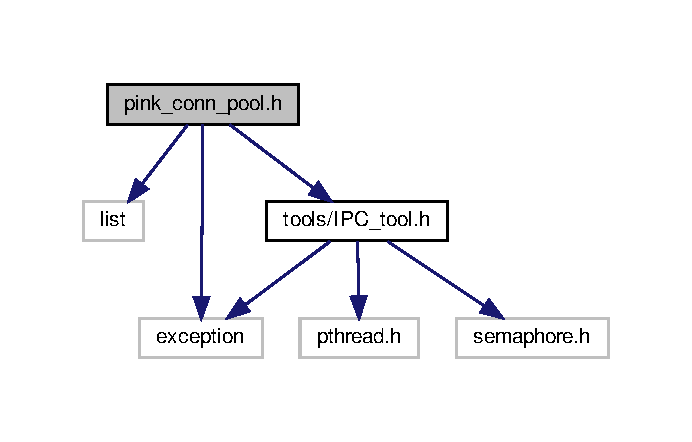
\includegraphics[width=332pt]{pink__conn__pool_8h__incl}
\end{center}
\end{figure}
This graph shows which files directly or indirectly include this file\+:\nopagebreak
\begin{figure}[H]
\begin{center}
\leavevmode
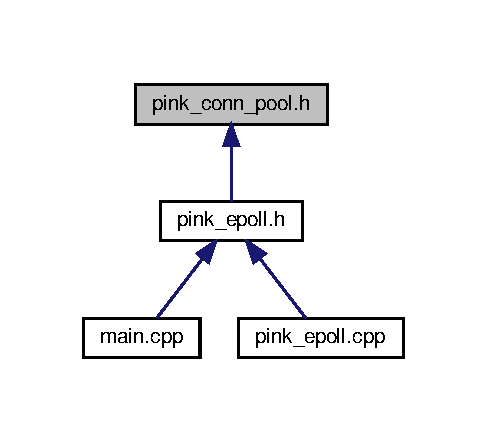
\includegraphics[width=234pt]{pink__conn__pool_8h__dep__incl}
\end{center}
\end{figure}
\subsection*{Classes}
\begin{DoxyCompactItemize}
\item 
class \hyperlink{classpink__conn__pool}{pink\+\_\+conn\+\_\+pool$<$ T $>$}
\end{DoxyCompactItemize}

\hypertarget{pink__conn__timer_8h}{}\section{pink\+\_\+conn\+\_\+timer.\+h File Reference}
\label{pink__conn__timer_8h}\index{pink\+\_\+conn\+\_\+timer.\+h@{pink\+\_\+conn\+\_\+timer.\+h}}
{\ttfamily \#include $<$time.\+h$>$}\newline
Include dependency graph for pink\+\_\+conn\+\_\+timer.\+h\+:
\nopagebreak
\begin{figure}[H]
\begin{center}
\leavevmode
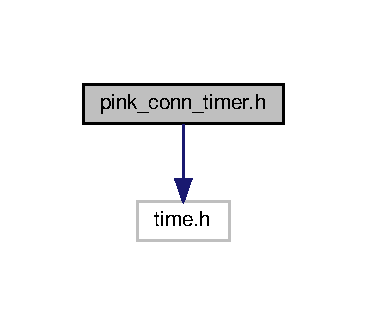
\includegraphics[width=176pt]{pink__conn__timer_8h__incl}
\end{center}
\end{figure}
This graph shows which files directly or indirectly include this file\+:
\nopagebreak
\begin{figure}[H]
\begin{center}
\leavevmode
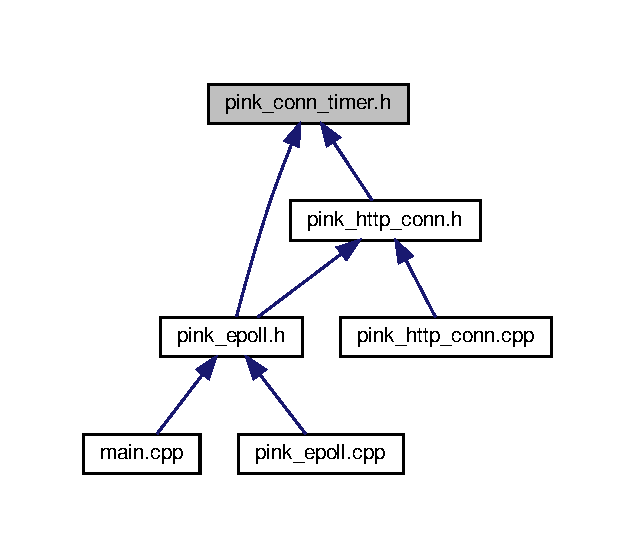
\includegraphics[width=305pt]{pink__conn__timer_8h__dep__incl}
\end{center}
\end{figure}
\subsection*{Classes}
\begin{DoxyCompactItemize}
\item 
class \hyperlink{classconn__timer}{conn\+\_\+timer}
\end{DoxyCompactItemize}

\hypertarget{pink__epoll_8cpp}{}\section{pink\+\_\+epoll.\+cpp File Reference}
\label{pink__epoll_8cpp}\index{pink\+\_\+epoll.\+cpp@{pink\+\_\+epoll.\+cpp}}
{\ttfamily \#include \char`\"{}pink\+\_\+epoll.\+h\char`\"{}}\newline
Include dependency graph for pink\+\_\+epoll.\+cpp\+:\nopagebreak
\begin{figure}[H]
\begin{center}
\leavevmode
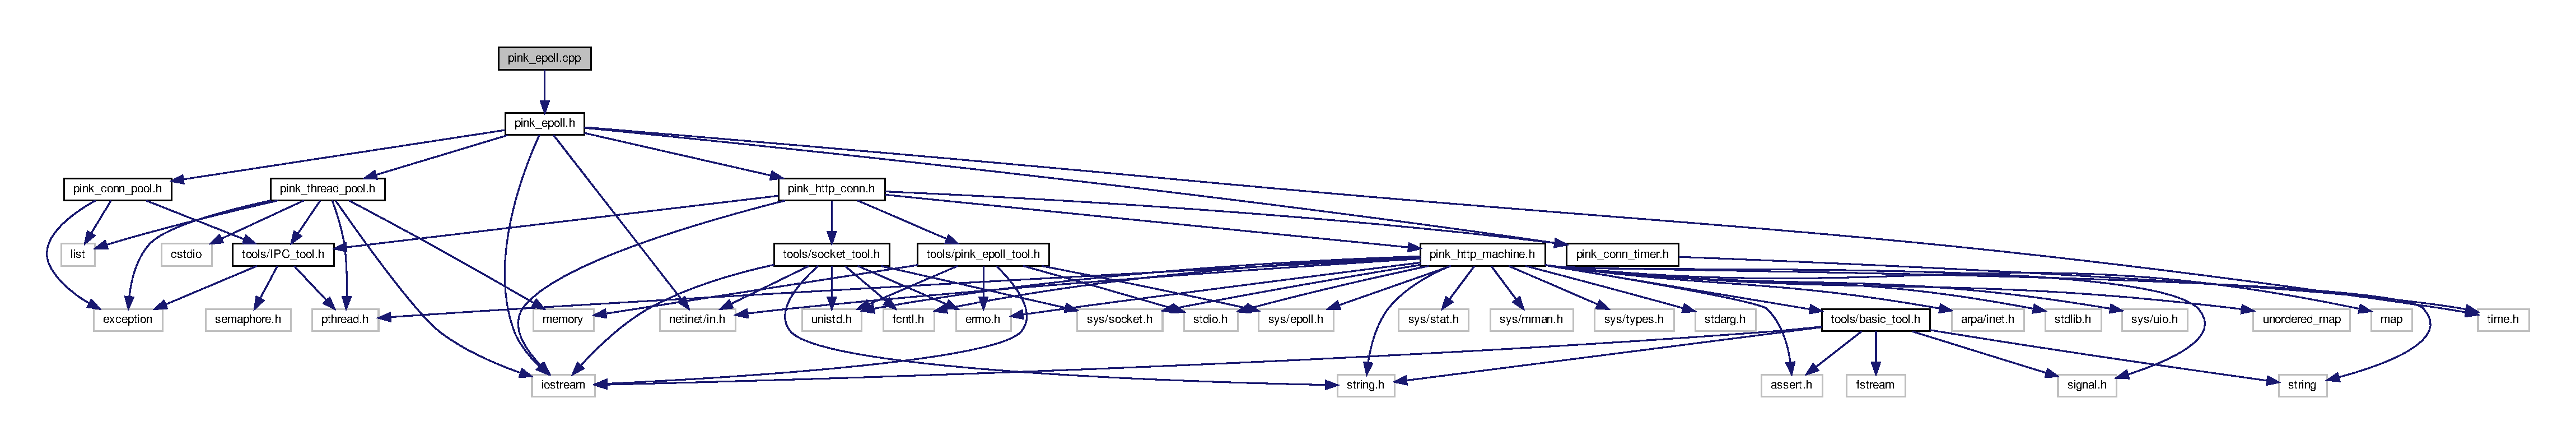
\includegraphics[width=350pt]{pink__epoll_8cpp__incl}
\end{center}
\end{figure}
\subsection*{Functions}
\begin{DoxyCompactItemize}
\item 
void \hyperlink{pink__epoll_8cpp_a756b8a3bffadb65045999bd5728f474a}{delete\+\_\+cb\+\_\+func} (\hyperlink{classpink__http__conn}{pink\+\_\+http\+\_\+conn} $\ast$conn)
\item 
int \hyperlink{pink__epoll_8cpp_ad15841527db9c5d3cc800ac21f750f23}{epoll\+\_\+run} (int epollfd, int listenfd)
\item 
void \hyperlink{pink__epoll_8cpp_ae30dffd8bcb9e6901638b8174108e760}{epoll\+\_\+et} (int epollfd, int listenfd)
\item 
void \hyperlink{pink__epoll_8cpp_a56d0d7b624f8626293e482ff84181800}{epoll\+\_\+lt} (int epollfd, int listenfd)
\end{DoxyCompactItemize}
\subsection*{Variables}
\begin{DoxyCompactItemize}
\item 
\hyperlink{basic__tool_8h_aa8adc7b5bceb1e76cda9b5ec5471159a}{conf\+\_\+t} \hyperlink{pink__epoll_8cpp_a40e427255962e28d8913a56db7b748b8}{conf}
\item 
struct epoll\+\_\+event $\ast$ \hyperlink{pink__epoll_8cpp_a18bcd14e4d4cab5184d3b046754cd248}{events}
\item 
bool \hyperlink{pink__epoll_8cpp_a10b9d1b41a98232e6a6e12873fcaa3c0}{stop\+\_\+server} = false
\item 
unique\+\_\+ptr$<$ \hyperlink{classpink__threadpool}{pink\+\_\+threadpool}$<$ \hyperlink{classpink__http__conn}{pink\+\_\+http\+\_\+conn} $>$ $>$ \hyperlink{pink__epoll_8cpp_ad535274fc8dfcf757689fa8a1375dc09}{t\+\_\+pool} = nullptr
\item 
unique\+\_\+ptr$<$ \hyperlink{classpink__time__heap}{pink\+\_\+time\+\_\+heap} $>$ \hyperlink{pink__epoll_8cpp_add757f95216eb53afab4c7623c2dd30c}{time\+\_\+heap} = nullptr
\item 
unique\+\_\+ptr$<$ \hyperlink{classpink__conn__pool}{pink\+\_\+conn\+\_\+pool}$<$ \hyperlink{classpink__http__conn}{pink\+\_\+http\+\_\+conn} $>$ $>$ \hyperlink{pink__epoll_8cpp_aabd90ecb53195c2ccf8e087e4a0c25fc}{c\+\_\+pool} = nullptr
\end{DoxyCompactItemize}


\subsection{Function Documentation}
\mbox{\Hypertarget{pink__epoll_8cpp_a756b8a3bffadb65045999bd5728f474a}\label{pink__epoll_8cpp_a756b8a3bffadb65045999bd5728f474a}} 
\index{pink\+\_\+epoll.\+cpp@{pink\+\_\+epoll.\+cpp}!delete\+\_\+cb\+\_\+func@{delete\+\_\+cb\+\_\+func}}
\index{delete\+\_\+cb\+\_\+func@{delete\+\_\+cb\+\_\+func}!pink\+\_\+epoll.\+cpp@{pink\+\_\+epoll.\+cpp}}
\subsubsection{\texorpdfstring{delete\+\_\+cb\+\_\+func()}{delete\_cb\_func()}}
{\footnotesize\ttfamily void delete\+\_\+cb\+\_\+func (\begin{DoxyParamCaption}\item[{\hyperlink{classpink__http__conn}{pink\+\_\+http\+\_\+conn} $\ast$}]{conn }\end{DoxyParamCaption})}



Definition at line 11 of file pink\+\_\+epoll.\+cpp.

Here is the caller graph for this function\+:\nopagebreak
\begin{figure}[H]
\begin{center}
\leavevmode
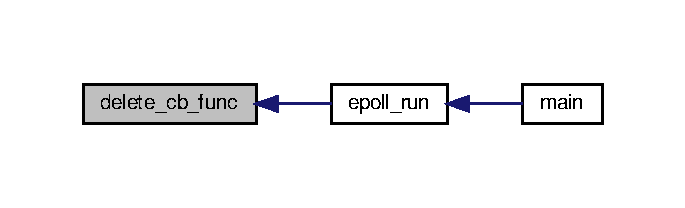
\includegraphics[width=329pt]{pink__epoll_8cpp_a756b8a3bffadb65045999bd5728f474a_icgraph}
\end{center}
\end{figure}
\mbox{\Hypertarget{pink__epoll_8cpp_ae30dffd8bcb9e6901638b8174108e760}\label{pink__epoll_8cpp_ae30dffd8bcb9e6901638b8174108e760}} 
\index{pink\+\_\+epoll.\+cpp@{pink\+\_\+epoll.\+cpp}!epoll\+\_\+et@{epoll\+\_\+et}}
\index{epoll\+\_\+et@{epoll\+\_\+et}!pink\+\_\+epoll.\+cpp@{pink\+\_\+epoll.\+cpp}}
\subsubsection{\texorpdfstring{epoll\+\_\+et()}{epoll\_et()}}
{\footnotesize\ttfamily void epoll\+\_\+et (\begin{DoxyParamCaption}\item[{int}]{epollfd,  }\item[{int}]{listenfd }\end{DoxyParamCaption})}



Definition at line 48 of file pink\+\_\+epoll.\+cpp.

Here is the call graph for this function\+:\nopagebreak
\begin{figure}[H]
\begin{center}
\leavevmode
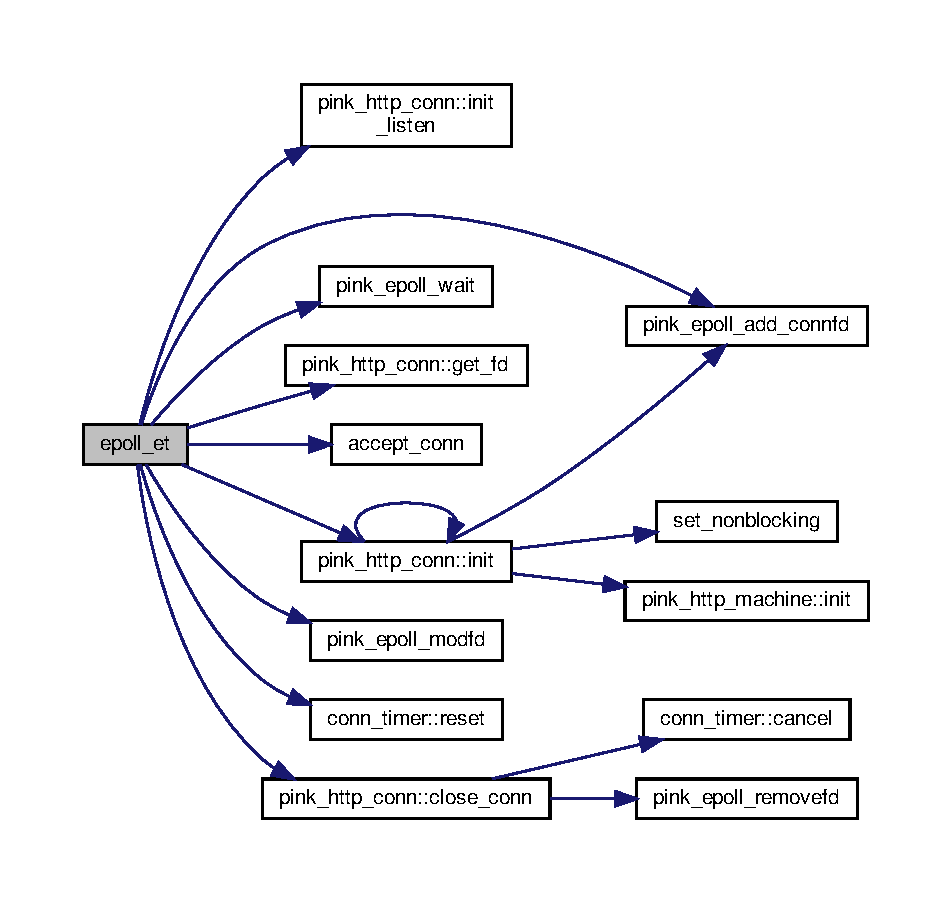
\includegraphics[width=350pt]{pink__epoll_8cpp_ae30dffd8bcb9e6901638b8174108e760_cgraph}
\end{center}
\end{figure}
Here is the caller graph for this function\+:\nopagebreak
\begin{figure}[H]
\begin{center}
\leavevmode
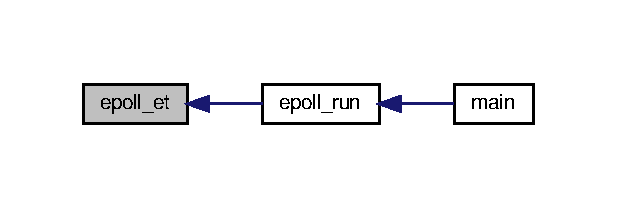
\includegraphics[width=296pt]{pink__epoll_8cpp_ae30dffd8bcb9e6901638b8174108e760_icgraph}
\end{center}
\end{figure}
\mbox{\Hypertarget{pink__epoll_8cpp_a56d0d7b624f8626293e482ff84181800}\label{pink__epoll_8cpp_a56d0d7b624f8626293e482ff84181800}} 
\index{pink\+\_\+epoll.\+cpp@{pink\+\_\+epoll.\+cpp}!epoll\+\_\+lt@{epoll\+\_\+lt}}
\index{epoll\+\_\+lt@{epoll\+\_\+lt}!pink\+\_\+epoll.\+cpp@{pink\+\_\+epoll.\+cpp}}
\subsubsection{\texorpdfstring{epoll\+\_\+lt()}{epoll\_lt()}}
{\footnotesize\ttfamily void epoll\+\_\+lt (\begin{DoxyParamCaption}\item[{int}]{epollfd,  }\item[{int}]{listenfd }\end{DoxyParamCaption})}



Definition at line 121 of file pink\+\_\+epoll.\+cpp.

Here is the call graph for this function\+:
\nopagebreak
\begin{figure}[H]
\begin{center}
\leavevmode
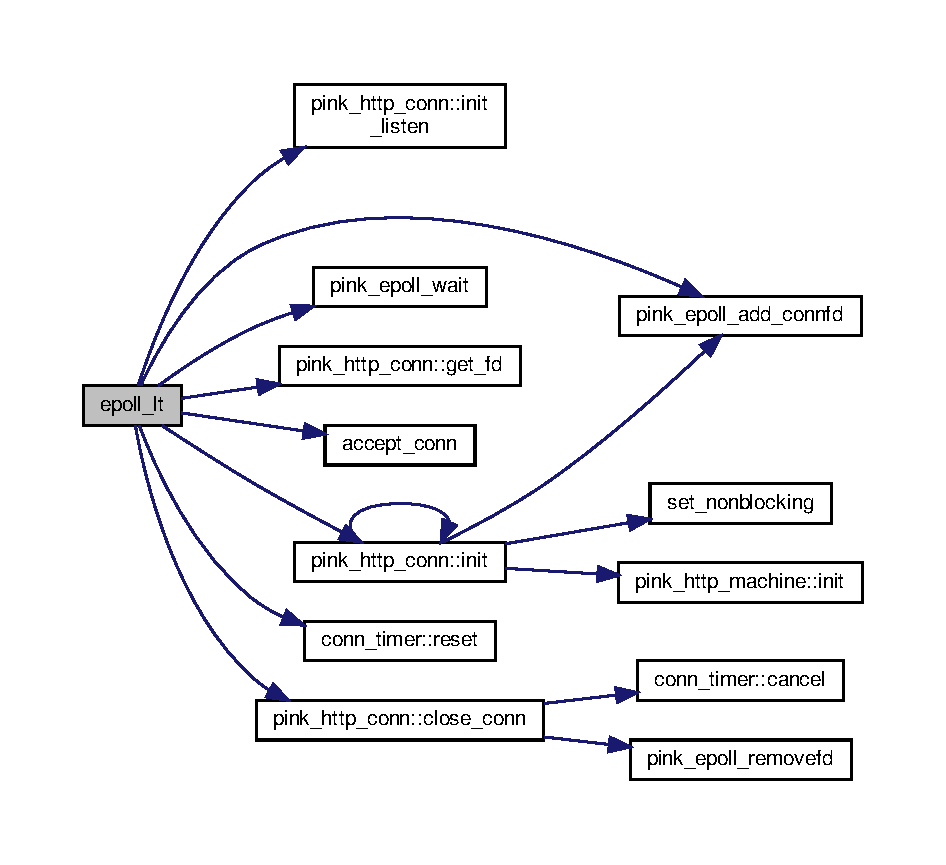
\includegraphics[width=350pt]{pink__epoll_8cpp_a56d0d7b624f8626293e482ff84181800_cgraph}
\end{center}
\end{figure}
Here is the caller graph for this function\+:
\nopagebreak
\begin{figure}[H]
\begin{center}
\leavevmode
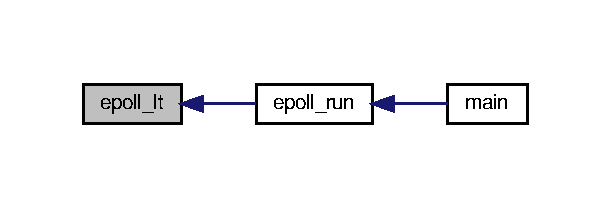
\includegraphics[width=293pt]{pink__epoll_8cpp_a56d0d7b624f8626293e482ff84181800_icgraph}
\end{center}
\end{figure}
\mbox{\Hypertarget{pink__epoll_8cpp_ad15841527db9c5d3cc800ac21f750f23}\label{pink__epoll_8cpp_ad15841527db9c5d3cc800ac21f750f23}} 
\index{pink\+\_\+epoll.\+cpp@{pink\+\_\+epoll.\+cpp}!epoll\+\_\+run@{epoll\+\_\+run}}
\index{epoll\+\_\+run@{epoll\+\_\+run}!pink\+\_\+epoll.\+cpp@{pink\+\_\+epoll.\+cpp}}
\subsubsection{\texorpdfstring{epoll\+\_\+run()}{epoll\_run()}}
{\footnotesize\ttfamily int epoll\+\_\+run (\begin{DoxyParamCaption}\item[{int}]{epollfd,  }\item[{int}]{listenfd }\end{DoxyParamCaption})}



Definition at line 15 of file pink\+\_\+epoll.\+cpp.

Here is the call graph for this function\+:
\nopagebreak
\begin{figure}[H]
\begin{center}
\leavevmode
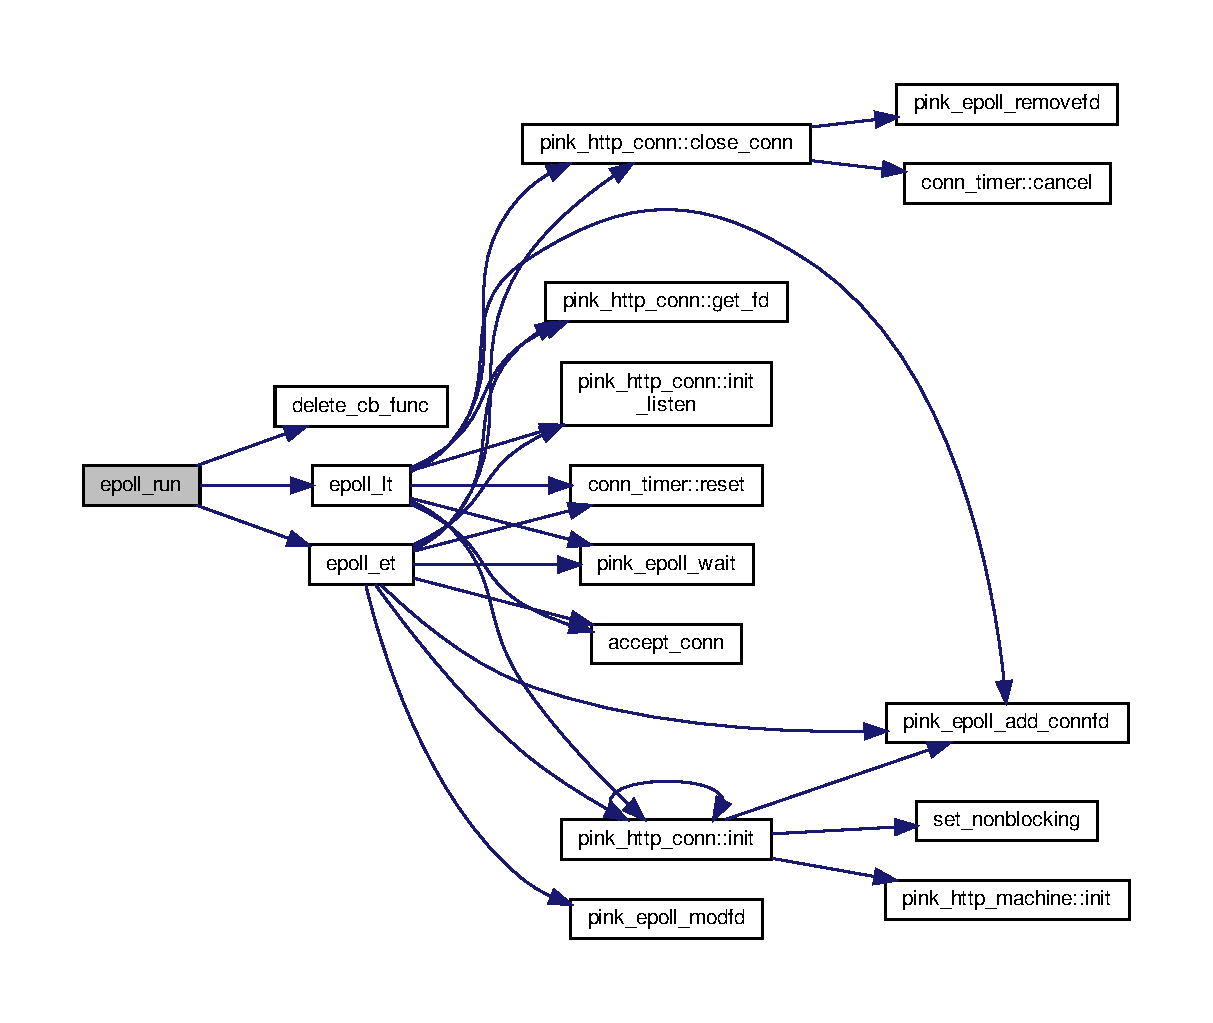
\includegraphics[width=350pt]{pink__epoll_8cpp_ad15841527db9c5d3cc800ac21f750f23_cgraph}
\end{center}
\end{figure}
Here is the caller graph for this function\+:
\nopagebreak
\begin{figure}[H]
\begin{center}
\leavevmode
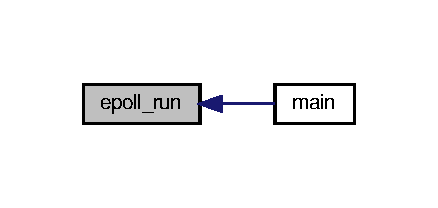
\includegraphics[width=210pt]{pink__epoll_8cpp_ad15841527db9c5d3cc800ac21f750f23_icgraph}
\end{center}
\end{figure}


\subsection{Variable Documentation}
\mbox{\Hypertarget{pink__epoll_8cpp_aabd90ecb53195c2ccf8e087e4a0c25fc}\label{pink__epoll_8cpp_aabd90ecb53195c2ccf8e087e4a0c25fc}} 
\index{pink\+\_\+epoll.\+cpp@{pink\+\_\+epoll.\+cpp}!c\+\_\+pool@{c\+\_\+pool}}
\index{c\+\_\+pool@{c\+\_\+pool}!pink\+\_\+epoll.\+cpp@{pink\+\_\+epoll.\+cpp}}
\subsubsection{\texorpdfstring{c\+\_\+pool}{c\_pool}}
{\footnotesize\ttfamily unique\+\_\+ptr$<$\hyperlink{classpink__conn__pool}{pink\+\_\+conn\+\_\+pool}$<$\hyperlink{classpink__http__conn}{pink\+\_\+http\+\_\+conn}$>$ $>$ c\+\_\+pool = nullptr}



Definition at line 9 of file pink\+\_\+epoll.\+cpp.

\mbox{\Hypertarget{pink__epoll_8cpp_a40e427255962e28d8913a56db7b748b8}\label{pink__epoll_8cpp_a40e427255962e28d8913a56db7b748b8}} 
\index{pink\+\_\+epoll.\+cpp@{pink\+\_\+epoll.\+cpp}!conf@{conf}}
\index{conf@{conf}!pink\+\_\+epoll.\+cpp@{pink\+\_\+epoll.\+cpp}}
\subsubsection{\texorpdfstring{conf}{conf}}
{\footnotesize\ttfamily \hyperlink{basic__tool_8h_aa8adc7b5bceb1e76cda9b5ec5471159a}{conf\+\_\+t} conf}



Definition at line 7 of file main.\+cpp.

\mbox{\Hypertarget{pink__epoll_8cpp_a18bcd14e4d4cab5184d3b046754cd248}\label{pink__epoll_8cpp_a18bcd14e4d4cab5184d3b046754cd248}} 
\index{pink\+\_\+epoll.\+cpp@{pink\+\_\+epoll.\+cpp}!events@{events}}
\index{events@{events}!pink\+\_\+epoll.\+cpp@{pink\+\_\+epoll.\+cpp}}
\subsubsection{\texorpdfstring{events}{events}}
{\footnotesize\ttfamily struct epoll\+\_\+event$\ast$ events}



Definition at line 3 of file pink\+\_\+epoll\+\_\+tool.\+cpp.

\mbox{\Hypertarget{pink__epoll_8cpp_a10b9d1b41a98232e6a6e12873fcaa3c0}\label{pink__epoll_8cpp_a10b9d1b41a98232e6a6e12873fcaa3c0}} 
\index{pink\+\_\+epoll.\+cpp@{pink\+\_\+epoll.\+cpp}!stop\+\_\+server@{stop\+\_\+server}}
\index{stop\+\_\+server@{stop\+\_\+server}!pink\+\_\+epoll.\+cpp@{pink\+\_\+epoll.\+cpp}}
\subsubsection{\texorpdfstring{stop\+\_\+server}{stop\_server}}
{\footnotesize\ttfamily bool stop\+\_\+server = false}



Definition at line 5 of file pink\+\_\+epoll.\+cpp.

\mbox{\Hypertarget{pink__epoll_8cpp_ad535274fc8dfcf757689fa8a1375dc09}\label{pink__epoll_8cpp_ad535274fc8dfcf757689fa8a1375dc09}} 
\index{pink\+\_\+epoll.\+cpp@{pink\+\_\+epoll.\+cpp}!t\+\_\+pool@{t\+\_\+pool}}
\index{t\+\_\+pool@{t\+\_\+pool}!pink\+\_\+epoll.\+cpp@{pink\+\_\+epoll.\+cpp}}
\subsubsection{\texorpdfstring{t\+\_\+pool}{t\_pool}}
{\footnotesize\ttfamily unique\+\_\+ptr$<$\hyperlink{classpink__threadpool}{pink\+\_\+threadpool}$<$\hyperlink{classpink__http__conn}{pink\+\_\+http\+\_\+conn}$>$ $>$ t\+\_\+pool = nullptr}



Definition at line 7 of file pink\+\_\+epoll.\+cpp.

\mbox{\Hypertarget{pink__epoll_8cpp_add757f95216eb53afab4c7623c2dd30c}\label{pink__epoll_8cpp_add757f95216eb53afab4c7623c2dd30c}} 
\index{pink\+\_\+epoll.\+cpp@{pink\+\_\+epoll.\+cpp}!time\+\_\+heap@{time\+\_\+heap}}
\index{time\+\_\+heap@{time\+\_\+heap}!pink\+\_\+epoll.\+cpp@{pink\+\_\+epoll.\+cpp}}
\subsubsection{\texorpdfstring{time\+\_\+heap}{time\_heap}}
{\footnotesize\ttfamily unique\+\_\+ptr$<$\hyperlink{classpink__time__heap}{pink\+\_\+time\+\_\+heap}$>$ time\+\_\+heap = nullptr}



Definition at line 8 of file pink\+\_\+epoll.\+cpp.


\hypertarget{pink__epoll_8h}{}\section{pink\+\_\+epoll.\+h File Reference}
\label{pink__epoll_8h}\index{pink\+\_\+epoll.\+h@{pink\+\_\+epoll.\+h}}
{\ttfamily \#include $<$netinet/in.\+h$>$}\newline
{\ttfamily \#include \char`\"{}pink\+\_\+thread\+\_\+pool.\+h\char`\"{}}\newline
{\ttfamily \#include \char`\"{}pink\+\_\+conn\+\_\+pool.\+h\char`\"{}}\newline
{\ttfamily \#include \char`\"{}pink\+\_\+http\+\_\+conn.\+h\char`\"{}}\newline
{\ttfamily \#include $<$iostream$>$}\newline
{\ttfamily \#include $<$time.\+h$>$}\newline
{\ttfamily \#include \char`\"{}pink\+\_\+conn\+\_\+timer.\+h\char`\"{}}\newline
Include dependency graph for pink\+\_\+epoll.\+h\+:\nopagebreak
\begin{figure}[H]
\begin{center}
\leavevmode
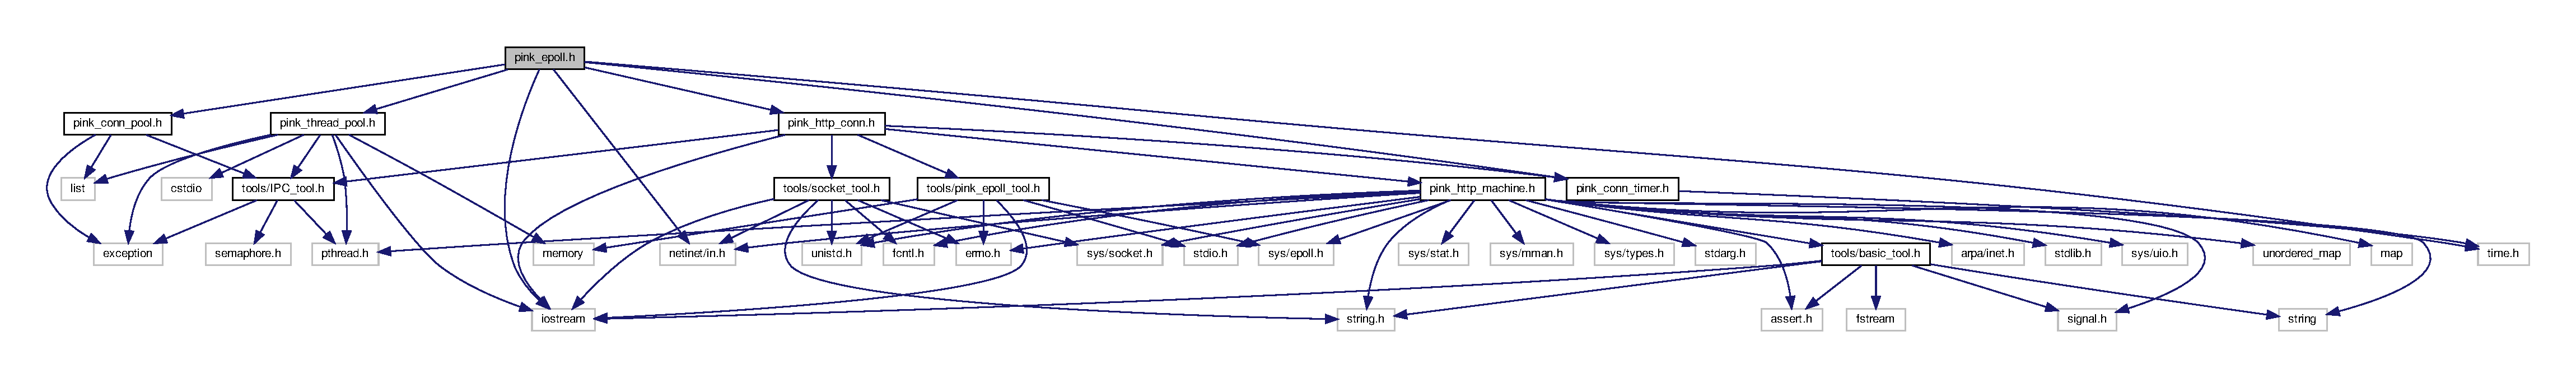
\includegraphics[width=350pt]{pink__epoll_8h__incl}
\end{center}
\end{figure}
This graph shows which files directly or indirectly include this file\+:\nopagebreak
\begin{figure}[H]
\begin{center}
\leavevmode
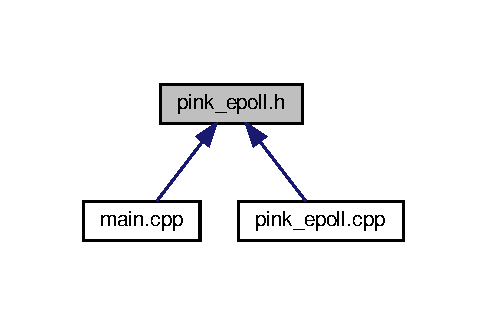
\includegraphics[width=234pt]{pink__epoll_8h__dep__incl}
\end{center}
\end{figure}
\subsection*{Classes}
\begin{DoxyCompactItemize}
\item 
class \hyperlink{classpink__time__heap}{pink\+\_\+time\+\_\+heap}
\end{DoxyCompactItemize}
\subsection*{Functions}
\begin{DoxyCompactItemize}
\item 
int \hyperlink{pink__epoll_8h_ad15841527db9c5d3cc800ac21f750f23}{epoll\+\_\+run} (int epollfd, int listenfd)
\item 
void \hyperlink{pink__epoll_8h_ae30dffd8bcb9e6901638b8174108e760}{epoll\+\_\+et} (int epollfd, int listenfd)
\item 
void \hyperlink{pink__epoll_8h_a56d0d7b624f8626293e482ff84181800}{epoll\+\_\+lt} (int epollfd, int listenfd)
\end{DoxyCompactItemize}


\subsection{Function Documentation}
\mbox{\Hypertarget{pink__epoll_8h_ae30dffd8bcb9e6901638b8174108e760}\label{pink__epoll_8h_ae30dffd8bcb9e6901638b8174108e760}} 
\index{pink\+\_\+epoll.\+h@{pink\+\_\+epoll.\+h}!epoll\+\_\+et@{epoll\+\_\+et}}
\index{epoll\+\_\+et@{epoll\+\_\+et}!pink\+\_\+epoll.\+h@{pink\+\_\+epoll.\+h}}
\subsubsection{\texorpdfstring{epoll\+\_\+et()}{epoll\_et()}}
{\footnotesize\ttfamily void epoll\+\_\+et (\begin{DoxyParamCaption}\item[{int}]{epollfd,  }\item[{int}]{listenfd }\end{DoxyParamCaption})}



Definition at line 48 of file pink\+\_\+epoll.\+cpp.

Here is the call graph for this function\+:\nopagebreak
\begin{figure}[H]
\begin{center}
\leavevmode
\includegraphics[width=350pt]{pink__epoll_8h_ae30dffd8bcb9e6901638b8174108e760_cgraph}
\end{center}
\end{figure}
Here is the caller graph for this function\+:\nopagebreak
\begin{figure}[H]
\begin{center}
\leavevmode
\includegraphics[width=296pt]{pink__epoll_8h_ae30dffd8bcb9e6901638b8174108e760_icgraph}
\end{center}
\end{figure}
\mbox{\Hypertarget{pink__epoll_8h_a56d0d7b624f8626293e482ff84181800}\label{pink__epoll_8h_a56d0d7b624f8626293e482ff84181800}} 
\index{pink\+\_\+epoll.\+h@{pink\+\_\+epoll.\+h}!epoll\+\_\+lt@{epoll\+\_\+lt}}
\index{epoll\+\_\+lt@{epoll\+\_\+lt}!pink\+\_\+epoll.\+h@{pink\+\_\+epoll.\+h}}
\subsubsection{\texorpdfstring{epoll\+\_\+lt()}{epoll\_lt()}}
{\footnotesize\ttfamily void epoll\+\_\+lt (\begin{DoxyParamCaption}\item[{int}]{epollfd,  }\item[{int}]{listenfd }\end{DoxyParamCaption})}

Here is the caller graph for this function\+:
\nopagebreak
\begin{figure}[H]
\begin{center}
\leavevmode
\includegraphics[width=293pt]{pink__epoll_8h_a56d0d7b624f8626293e482ff84181800_icgraph}
\end{center}
\end{figure}
\mbox{\Hypertarget{pink__epoll_8h_ad15841527db9c5d3cc800ac21f750f23}\label{pink__epoll_8h_ad15841527db9c5d3cc800ac21f750f23}} 
\index{pink\+\_\+epoll.\+h@{pink\+\_\+epoll.\+h}!epoll\+\_\+run@{epoll\+\_\+run}}
\index{epoll\+\_\+run@{epoll\+\_\+run}!pink\+\_\+epoll.\+h@{pink\+\_\+epoll.\+h}}
\subsubsection{\texorpdfstring{epoll\+\_\+run()}{epoll\_run()}}
{\footnotesize\ttfamily int epoll\+\_\+run (\begin{DoxyParamCaption}\item[{int}]{epollfd,  }\item[{int}]{listenfd }\end{DoxyParamCaption})}



Definition at line 15 of file pink\+\_\+epoll.\+cpp.

Here is the call graph for this function\+:
\nopagebreak
\begin{figure}[H]
\begin{center}
\leavevmode
\includegraphics[width=350pt]{pink__epoll_8h_ad15841527db9c5d3cc800ac21f750f23_cgraph}
\end{center}
\end{figure}
Here is the caller graph for this function\+:
\nopagebreak
\begin{figure}[H]
\begin{center}
\leavevmode
\includegraphics[width=210pt]{pink__epoll_8h_ad15841527db9c5d3cc800ac21f750f23_icgraph}
\end{center}
\end{figure}

\hypertarget{pink__http__conn_8cpp}{}\section{pink\+\_\+http\+\_\+conn.\+cpp File Reference}
\label{pink__http__conn_8cpp}\index{pink\+\_\+http\+\_\+conn.\+cpp@{pink\+\_\+http\+\_\+conn.\+cpp}}
{\ttfamily \#include \char`\"{}pink\+\_\+http\+\_\+conn.\+h\char`\"{}}\newline
Include dependency graph for pink\+\_\+http\+\_\+conn.\+cpp\+:
\nopagebreak
\begin{figure}[H]
\begin{center}
\leavevmode
\includegraphics[width=350pt]{pink__http__conn_8cpp__incl}
\end{center}
\end{figure}

\hypertarget{pink__http__conn_8h}{}\section{pink\+\_\+http\+\_\+conn.\+h File Reference}
\label{pink__http__conn_8h}\index{pink\+\_\+http\+\_\+conn.\+h@{pink\+\_\+http\+\_\+conn.\+h}}
{\ttfamily \#include $<$iostream$>$}\newline
{\ttfamily \#include \char`\"{}tools/\+I\+P\+C\+\_\+tool.\+h\char`\"{}}\newline
{\ttfamily \#include \char`\"{}tools/socket\+\_\+tool.\+h\char`\"{}}\newline
{\ttfamily \#include \char`\"{}tools/pink\+\_\+epoll\+\_\+tool.\+h\char`\"{}}\newline
{\ttfamily \#include \char`\"{}pink\+\_\+http\+\_\+machine.\+h\char`\"{}}\newline
{\ttfamily \#include \char`\"{}pink\+\_\+conn\+\_\+timer.\+h\char`\"{}}\newline
Include dependency graph for pink\+\_\+http\+\_\+conn.\+h\+:
\nopagebreak
\begin{figure}[H]
\begin{center}
\leavevmode
\includegraphics[width=350pt]{pink__http__conn_8h__incl}
\end{center}
\end{figure}
This graph shows which files directly or indirectly include this file\+:
\nopagebreak
\begin{figure}[H]
\begin{center}
\leavevmode
\includegraphics[width=305pt]{pink__http__conn_8h__dep__incl}
\end{center}
\end{figure}
\subsection*{Classes}
\begin{DoxyCompactItemize}
\item 
class \hyperlink{classpink__http__conn}{pink\+\_\+http\+\_\+conn}
\end{DoxyCompactItemize}

\hypertarget{pink__http__machine_8cpp}{}\section{pink\+\_\+http\+\_\+machine.\+cpp File Reference}
\label{pink__http__machine_8cpp}\index{pink\+\_\+http\+\_\+machine.\+cpp@{pink\+\_\+http\+\_\+machine.\+cpp}}
{\ttfamily \#include \char`\"{}pink\+\_\+http\+\_\+machine.\+h\char`\"{}}\newline
Include dependency graph for pink\+\_\+http\+\_\+machine.\+cpp\+:\nopagebreak
\begin{figure}[H]
\begin{center}
\leavevmode
\includegraphics[width=350pt]{pink__http__machine_8cpp__incl}
\end{center}
\end{figure}
\subsection*{Functions}
\begin{DoxyCompactItemize}
\item 
bool \hyperlink{pink__http__machine_8cpp_a9a6484ca3021c09b306a1752e8d2f2d7}{check\+\_\+and\+\_\+move} (char $\ast$\&text, const char $\ast$prefix)
\end{DoxyCompactItemize}
\subsection*{Variables}
\begin{DoxyCompactItemize}
\item 
const char $\ast$ \hyperlink{pink__http__machine_8cpp_a2920c19c4461f3dcfc79963bcf5129fa}{ok\+\_\+200\+\_\+title} = \char`\"{}OK\char`\"{}
\item 
const char $\ast$ \hyperlink{pink__http__machine_8cpp_a528c20fe7f72b626cc4a04d84d2d2b03}{error\+\_\+400\+\_\+title} = \char`\"{}Bad Request\char`\"{}
\item 
const char $\ast$ \hyperlink{pink__http__machine_8cpp_a43f51c2142748f1f9c418546c180238c}{error\+\_\+400\+\_\+form} = \char`\"{}Your request has bad syntax or is inherently impossible to satisfy.\textbackslash{}n\char`\"{}
\item 
const char $\ast$ \hyperlink{pink__http__machine_8cpp_acd4d47a5e72f592b4cb6e90b35266cdd}{error\+\_\+403\+\_\+title} = \char`\"{}Forbidden\char`\"{}
\item 
const char $\ast$ \hyperlink{pink__http__machine_8cpp_a0a883d39716510bc46358e62aefed870}{error\+\_\+403\+\_\+form} = \char`\"{}You do not have permission to get the file from this server.\textbackslash{}n\char`\"{}
\item 
const char $\ast$ \hyperlink{pink__http__machine_8cpp_a2a610d885819a1c9a250c8d0d1c2af11}{error\+\_\+404\+\_\+title} = \char`\"{}Not Found\char`\"{}
\item 
const char $\ast$ \hyperlink{pink__http__machine_8cpp_ab1f9deece0fcb4980efc837e2386774f}{error\+\_\+404\+\_\+form} = \char`\"{}The requested file was not found on this server.\textbackslash{}n\char`\"{}
\item 
const char $\ast$ \hyperlink{pink__http__machine_8cpp_ae0c5b89b5e87bf8b9e8860ce6e977250}{error\+\_\+500\+\_\+title} = \char`\"{}Internal Error\char`\"{}
\item 
const char $\ast$ \hyperlink{pink__http__machine_8cpp_a2ecfc4b77a046da5b99fd43d4fb58e81}{error\+\_\+500\+\_\+form} = \char`\"{}There was an unusual problem serving the requested file.\textbackslash{}n\char`\"{}
\item 
\hyperlink{basic__tool_8h_aa8adc7b5bceb1e76cda9b5ec5471159a}{conf\+\_\+t} \hyperlink{pink__http__machine_8cpp_a40e427255962e28d8913a56db7b748b8}{conf}
\end{DoxyCompactItemize}


\subsection{Function Documentation}
\mbox{\Hypertarget{pink__http__machine_8cpp_a9a6484ca3021c09b306a1752e8d2f2d7}\label{pink__http__machine_8cpp_a9a6484ca3021c09b306a1752e8d2f2d7}} 
\index{pink\+\_\+http\+\_\+machine.\+cpp@{pink\+\_\+http\+\_\+machine.\+cpp}!check\+\_\+and\+\_\+move@{check\+\_\+and\+\_\+move}}
\index{check\+\_\+and\+\_\+move@{check\+\_\+and\+\_\+move}!pink\+\_\+http\+\_\+machine.\+cpp@{pink\+\_\+http\+\_\+machine.\+cpp}}
\subsubsection{\texorpdfstring{check\+\_\+and\+\_\+move()}{check\_and\_move()}}
{\footnotesize\ttfamily bool check\+\_\+and\+\_\+move (\begin{DoxyParamCaption}\item[{char $\ast$\&}]{text,  }\item[{const char $\ast$}]{prefix }\end{DoxyParamCaption})\hspace{0.3cm}{\ttfamily [inline]}}



Definition at line 252 of file pink\+\_\+http\+\_\+machine.\+cpp.



\subsection{Variable Documentation}
\mbox{\Hypertarget{pink__http__machine_8cpp_a40e427255962e28d8913a56db7b748b8}\label{pink__http__machine_8cpp_a40e427255962e28d8913a56db7b748b8}} 
\index{pink\+\_\+http\+\_\+machine.\+cpp@{pink\+\_\+http\+\_\+machine.\+cpp}!conf@{conf}}
\index{conf@{conf}!pink\+\_\+http\+\_\+machine.\+cpp@{pink\+\_\+http\+\_\+machine.\+cpp}}
\subsubsection{\texorpdfstring{conf}{conf}}
{\footnotesize\ttfamily \hyperlink{basic__tool_8h_aa8adc7b5bceb1e76cda9b5ec5471159a}{conf\+\_\+t} conf}



Definition at line 7 of file main.\+cpp.

\mbox{\Hypertarget{pink__http__machine_8cpp_a43f51c2142748f1f9c418546c180238c}\label{pink__http__machine_8cpp_a43f51c2142748f1f9c418546c180238c}} 
\index{pink\+\_\+http\+\_\+machine.\+cpp@{pink\+\_\+http\+\_\+machine.\+cpp}!error\+\_\+400\+\_\+form@{error\+\_\+400\+\_\+form}}
\index{error\+\_\+400\+\_\+form@{error\+\_\+400\+\_\+form}!pink\+\_\+http\+\_\+machine.\+cpp@{pink\+\_\+http\+\_\+machine.\+cpp}}
\subsubsection{\texorpdfstring{error\+\_\+400\+\_\+form}{error\_400\_form}}
{\footnotesize\ttfamily const char$\ast$ error\+\_\+400\+\_\+form = \char`\"{}Your request has bad syntax or is inherently impossible to satisfy.\textbackslash{}n\char`\"{}}



Definition at line 10 of file pink\+\_\+http\+\_\+machine.\+cpp.

\mbox{\Hypertarget{pink__http__machine_8cpp_a528c20fe7f72b626cc4a04d84d2d2b03}\label{pink__http__machine_8cpp_a528c20fe7f72b626cc4a04d84d2d2b03}} 
\index{pink\+\_\+http\+\_\+machine.\+cpp@{pink\+\_\+http\+\_\+machine.\+cpp}!error\+\_\+400\+\_\+title@{error\+\_\+400\+\_\+title}}
\index{error\+\_\+400\+\_\+title@{error\+\_\+400\+\_\+title}!pink\+\_\+http\+\_\+machine.\+cpp@{pink\+\_\+http\+\_\+machine.\+cpp}}
\subsubsection{\texorpdfstring{error\+\_\+400\+\_\+title}{error\_400\_title}}
{\footnotesize\ttfamily const char$\ast$ error\+\_\+400\+\_\+title = \char`\"{}Bad Request\char`\"{}}



Definition at line 9 of file pink\+\_\+http\+\_\+machine.\+cpp.

\mbox{\Hypertarget{pink__http__machine_8cpp_a0a883d39716510bc46358e62aefed870}\label{pink__http__machine_8cpp_a0a883d39716510bc46358e62aefed870}} 
\index{pink\+\_\+http\+\_\+machine.\+cpp@{pink\+\_\+http\+\_\+machine.\+cpp}!error\+\_\+403\+\_\+form@{error\+\_\+403\+\_\+form}}
\index{error\+\_\+403\+\_\+form@{error\+\_\+403\+\_\+form}!pink\+\_\+http\+\_\+machine.\+cpp@{pink\+\_\+http\+\_\+machine.\+cpp}}
\subsubsection{\texorpdfstring{error\+\_\+403\+\_\+form}{error\_403\_form}}
{\footnotesize\ttfamily const char$\ast$ error\+\_\+403\+\_\+form = \char`\"{}You do not have permission to get the file from this server.\textbackslash{}n\char`\"{}}



Definition at line 12 of file pink\+\_\+http\+\_\+machine.\+cpp.

\mbox{\Hypertarget{pink__http__machine_8cpp_acd4d47a5e72f592b4cb6e90b35266cdd}\label{pink__http__machine_8cpp_acd4d47a5e72f592b4cb6e90b35266cdd}} 
\index{pink\+\_\+http\+\_\+machine.\+cpp@{pink\+\_\+http\+\_\+machine.\+cpp}!error\+\_\+403\+\_\+title@{error\+\_\+403\+\_\+title}}
\index{error\+\_\+403\+\_\+title@{error\+\_\+403\+\_\+title}!pink\+\_\+http\+\_\+machine.\+cpp@{pink\+\_\+http\+\_\+machine.\+cpp}}
\subsubsection{\texorpdfstring{error\+\_\+403\+\_\+title}{error\_403\_title}}
{\footnotesize\ttfamily const char$\ast$ error\+\_\+403\+\_\+title = \char`\"{}Forbidden\char`\"{}}



Definition at line 11 of file pink\+\_\+http\+\_\+machine.\+cpp.

\mbox{\Hypertarget{pink__http__machine_8cpp_ab1f9deece0fcb4980efc837e2386774f}\label{pink__http__machine_8cpp_ab1f9deece0fcb4980efc837e2386774f}} 
\index{pink\+\_\+http\+\_\+machine.\+cpp@{pink\+\_\+http\+\_\+machine.\+cpp}!error\+\_\+404\+\_\+form@{error\+\_\+404\+\_\+form}}
\index{error\+\_\+404\+\_\+form@{error\+\_\+404\+\_\+form}!pink\+\_\+http\+\_\+machine.\+cpp@{pink\+\_\+http\+\_\+machine.\+cpp}}
\subsubsection{\texorpdfstring{error\+\_\+404\+\_\+form}{error\_404\_form}}
{\footnotesize\ttfamily const char$\ast$ error\+\_\+404\+\_\+form = \char`\"{}The requested file was not found on this server.\textbackslash{}n\char`\"{}}



Definition at line 14 of file pink\+\_\+http\+\_\+machine.\+cpp.

\mbox{\Hypertarget{pink__http__machine_8cpp_a2a610d885819a1c9a250c8d0d1c2af11}\label{pink__http__machine_8cpp_a2a610d885819a1c9a250c8d0d1c2af11}} 
\index{pink\+\_\+http\+\_\+machine.\+cpp@{pink\+\_\+http\+\_\+machine.\+cpp}!error\+\_\+404\+\_\+title@{error\+\_\+404\+\_\+title}}
\index{error\+\_\+404\+\_\+title@{error\+\_\+404\+\_\+title}!pink\+\_\+http\+\_\+machine.\+cpp@{pink\+\_\+http\+\_\+machine.\+cpp}}
\subsubsection{\texorpdfstring{error\+\_\+404\+\_\+title}{error\_404\_title}}
{\footnotesize\ttfamily const char$\ast$ error\+\_\+404\+\_\+title = \char`\"{}Not Found\char`\"{}}



Definition at line 13 of file pink\+\_\+http\+\_\+machine.\+cpp.

\mbox{\Hypertarget{pink__http__machine_8cpp_a2ecfc4b77a046da5b99fd43d4fb58e81}\label{pink__http__machine_8cpp_a2ecfc4b77a046da5b99fd43d4fb58e81}} 
\index{pink\+\_\+http\+\_\+machine.\+cpp@{pink\+\_\+http\+\_\+machine.\+cpp}!error\+\_\+500\+\_\+form@{error\+\_\+500\+\_\+form}}
\index{error\+\_\+500\+\_\+form@{error\+\_\+500\+\_\+form}!pink\+\_\+http\+\_\+machine.\+cpp@{pink\+\_\+http\+\_\+machine.\+cpp}}
\subsubsection{\texorpdfstring{error\+\_\+500\+\_\+form}{error\_500\_form}}
{\footnotesize\ttfamily const char$\ast$ error\+\_\+500\+\_\+form = \char`\"{}There was an unusual problem serving the requested file.\textbackslash{}n\char`\"{}}



Definition at line 16 of file pink\+\_\+http\+\_\+machine.\+cpp.

\mbox{\Hypertarget{pink__http__machine_8cpp_ae0c5b89b5e87bf8b9e8860ce6e977250}\label{pink__http__machine_8cpp_ae0c5b89b5e87bf8b9e8860ce6e977250}} 
\index{pink\+\_\+http\+\_\+machine.\+cpp@{pink\+\_\+http\+\_\+machine.\+cpp}!error\+\_\+500\+\_\+title@{error\+\_\+500\+\_\+title}}
\index{error\+\_\+500\+\_\+title@{error\+\_\+500\+\_\+title}!pink\+\_\+http\+\_\+machine.\+cpp@{pink\+\_\+http\+\_\+machine.\+cpp}}
\subsubsection{\texorpdfstring{error\+\_\+500\+\_\+title}{error\_500\_title}}
{\footnotesize\ttfamily const char$\ast$ error\+\_\+500\+\_\+title = \char`\"{}Internal Error\char`\"{}}



Definition at line 15 of file pink\+\_\+http\+\_\+machine.\+cpp.

\mbox{\Hypertarget{pink__http__machine_8cpp_a2920c19c4461f3dcfc79963bcf5129fa}\label{pink__http__machine_8cpp_a2920c19c4461f3dcfc79963bcf5129fa}} 
\index{pink\+\_\+http\+\_\+machine.\+cpp@{pink\+\_\+http\+\_\+machine.\+cpp}!ok\+\_\+200\+\_\+title@{ok\+\_\+200\+\_\+title}}
\index{ok\+\_\+200\+\_\+title@{ok\+\_\+200\+\_\+title}!pink\+\_\+http\+\_\+machine.\+cpp@{pink\+\_\+http\+\_\+machine.\+cpp}}
\subsubsection{\texorpdfstring{ok\+\_\+200\+\_\+title}{ok\_200\_title}}
{\footnotesize\ttfamily const char$\ast$ ok\+\_\+200\+\_\+title = \char`\"{}OK\char`\"{}}



Definition at line 8 of file pink\+\_\+http\+\_\+machine.\+cpp.


\hypertarget{pink__http__machine_8h}{}\section{pink\+\_\+http\+\_\+machine.\+h File Reference}
\label{pink__http__machine_8h}\index{pink\+\_\+http\+\_\+machine.\+h@{pink\+\_\+http\+\_\+machine.\+h}}
{\ttfamily \#include $<$assert.\+h$>$}\newline
{\ttfamily \#include $<$sys/stat.\+h$>$}\newline
{\ttfamily \#include $<$sys/mman.\+h$>$}\newline
{\ttfamily \#include $<$sys/types.\+h$>$}\newline
{\ttfamily \#include $<$stdarg.\+h$>$}\newline
{\ttfamily \#include $<$errno.\+h$>$}\newline
{\ttfamily \#include $<$unistd.\+h$>$}\newline
{\ttfamily \#include $<$signal.\+h$>$}\newline
{\ttfamily \#include $<$sys/epoll.\+h$>$}\newline
{\ttfamily \#include $<$fcntl.\+h$>$}\newline
{\ttfamily \#include $<$sys/socket.\+h$>$}\newline
{\ttfamily \#include $<$netinet/in.\+h$>$}\newline
{\ttfamily \#include $<$arpa/inet.\+h$>$}\newline
{\ttfamily \#include $<$string.\+h$>$}\newline
{\ttfamily \#include $<$pthread.\+h$>$}\newline
{\ttfamily \#include $<$stdio.\+h$>$}\newline
{\ttfamily \#include $<$stdlib.\+h$>$}\newline
{\ttfamily \#include $<$sys/uio.\+h$>$}\newline
{\ttfamily \#include $<$string$>$}\newline
{\ttfamily \#include $<$unordered\+\_\+map$>$}\newline
{\ttfamily \#include $<$map$>$}\newline
{\ttfamily \#include \char`\"{}tools/basic\+\_\+tool.\+h\char`\"{}}\newline
Include dependency graph for pink\+\_\+http\+\_\+machine.\+h\+:
\nopagebreak
\begin{figure}[H]
\begin{center}
\leavevmode
\includegraphics[width=350pt]{pink__http__machine_8h__incl}
\end{center}
\end{figure}
This graph shows which files directly or indirectly include this file\+:
\nopagebreak
\begin{figure}[H]
\begin{center}
\leavevmode
\includegraphics[width=350pt]{pink__http__machine_8h__dep__incl}
\end{center}
\end{figure}
\subsection*{Classes}
\begin{DoxyCompactItemize}
\item 
class \hyperlink{classpink__http__machine}{pink\+\_\+http\+\_\+machine}
\end{DoxyCompactItemize}

\hypertarget{pink__mem__pool_8cpp}{}\section{pink\+\_\+mem\+\_\+pool.\+cpp File Reference}
\label{pink__mem__pool_8cpp}\index{pink\+\_\+mem\+\_\+pool.\+cpp@{pink\+\_\+mem\+\_\+pool.\+cpp}}

\hypertarget{pink__mem__pool_8h}{}\section{pink\+\_\+mem\+\_\+pool.\+h File Reference}
\label{pink__mem__pool_8h}\index{pink\+\_\+mem\+\_\+pool.\+h@{pink\+\_\+mem\+\_\+pool.\+h}}
{\ttfamily \#include $<$cstddef$>$}\newline
Include dependency graph for pink\+\_\+mem\+\_\+pool.\+h\+:\nopagebreak
\begin{figure}[H]
\begin{center}
\leavevmode
\includegraphics[width=173pt]{pink__mem__pool_8h__incl}
\end{center}
\end{figure}
\subsection*{Classes}
\begin{DoxyCompactItemize}
\item 
class \hyperlink{classpink__mem__pool}{pink\+\_\+mem\+\_\+pool}
\end{DoxyCompactItemize}
\subsection*{Variables}
\begin{DoxyCompactItemize}
\item 
class \hyperlink{classpink__mem__pool}{pink\+\_\+mem\+\_\+pool} \hyperlink{pink__mem__pool_8h_a3c17566ea2e0abb28c9693ee9da60cfd}{start\+\_\+free} = 0
\end{DoxyCompactItemize}


\subsection{Variable Documentation}
\mbox{\Hypertarget{pink__mem__pool_8h_a3c17566ea2e0abb28c9693ee9da60cfd}\label{pink__mem__pool_8h_a3c17566ea2e0abb28c9693ee9da60cfd}} 
\index{pink\+\_\+mem\+\_\+pool.\+h@{pink\+\_\+mem\+\_\+pool.\+h}!start\+\_\+free@{start\+\_\+free}}
\index{start\+\_\+free@{start\+\_\+free}!pink\+\_\+mem\+\_\+pool.\+h@{pink\+\_\+mem\+\_\+pool.\+h}}
\subsubsection{\texorpdfstring{start\+\_\+free}{start\_free}}
{\footnotesize\ttfamily class \hyperlink{classpink__mem__pool}{pink\+\_\+mem\+\_\+pool} start\+\_\+free = 0}


\hypertarget{pink__thread__pool_8h}{}\section{pink\+\_\+thread\+\_\+pool.\+h File Reference}
\label{pink__thread__pool_8h}\index{pink\+\_\+thread\+\_\+pool.\+h@{pink\+\_\+thread\+\_\+pool.\+h}}
{\ttfamily \#include $<$list$>$}\newline
{\ttfamily \#include $<$cstdio$>$}\newline
{\ttfamily \#include $<$exception$>$}\newline
{\ttfamily \#include $<$pthread.\+h$>$}\newline
{\ttfamily \#include $<$memory$>$}\newline
{\ttfamily \#include $<$iostream$>$}\newline
{\ttfamily \#include \char`\"{}tools/\+I\+P\+C\+\_\+tool.\+h\char`\"{}}\newline
Include dependency graph for pink\+\_\+thread\+\_\+pool.\+h\+:
\nopagebreak
\begin{figure}[H]
\begin{center}
\leavevmode
\includegraphics[width=350pt]{pink__thread__pool_8h__incl}
\end{center}
\end{figure}
This graph shows which files directly or indirectly include this file\+:
\nopagebreak
\begin{figure}[H]
\begin{center}
\leavevmode
\includegraphics[width=234pt]{pink__thread__pool_8h__dep__incl}
\end{center}
\end{figure}
\subsection*{Classes}
\begin{DoxyCompactItemize}
\item 
class \hyperlink{classpink__threadpool}{pink\+\_\+threadpool$<$ T $>$}
\end{DoxyCompactItemize}

\hypertarget{pressure__test_8cpp}{}\section{test/pressure\+\_\+test.cpp File Reference}
\label{pressure__test_8cpp}\index{test/pressure\+\_\+test.\+cpp@{test/pressure\+\_\+test.\+cpp}}
{\ttfamily \#include $<$stdlib.\+h$>$}\newline
{\ttfamily \#include $<$stdio.\+h$>$}\newline
{\ttfamily \#include $<$assert.\+h$>$}\newline
{\ttfamily \#include $<$unistd.\+h$>$}\newline
{\ttfamily \#include $<$sys/types.\+h$>$}\newline
{\ttfamily \#include $<$sys/epoll.\+h$>$}\newline
{\ttfamily \#include $<$fcntl.\+h$>$}\newline
{\ttfamily \#include $<$errno.\+h$>$}\newline
{\ttfamily \#include $<$sys/socket.\+h$>$}\newline
{\ttfamily \#include $<$netinet/in.\+h$>$}\newline
{\ttfamily \#include $<$arpa/inet.\+h$>$}\newline
{\ttfamily \#include $<$string.\+h$>$}\newline
{\ttfamily \#include $<$iostream$>$}\newline
Include dependency graph for pressure\+\_\+test.\+cpp\+:
\nopagebreak
\begin{figure}[H]
\begin{center}
\leavevmode
\includegraphics[width=350pt]{pressure__test_8cpp__incl}
\end{center}
\end{figure}
\subsection*{Functions}
\begin{DoxyCompactItemize}
\item 
int \hyperlink{pressure__test_8cpp_a450a9be7be692d8ac42f64acddbdaadd}{set\+\_\+nonblocking} (int fd)
\item 
void \hyperlink{pressure__test_8cpp_ad1c24852cf5a7763bce4dbfa3c2e02bc}{epoll\+\_\+addfd} (int epoll\+\_\+fd, int fd, const int \hyperlink{pink__epoll__tool_8cpp_a18bcd14e4d4cab5184d3b046754cd248}{events})
\item 
bool \hyperlink{pressure__test_8cpp_abb170baed7617879b86af54f38037426}{write\+\_\+nbytes} (int sockfd, const char $\ast$buffer, int len)
\item 
bool \hyperlink{pressure__test_8cpp_a6bf08c7e8bce05652661cb234feb0add}{read\+\_\+once} (int sockfd, char $\ast$buffer, int len)
\item 
void \hyperlink{pressure__test_8cpp_a8cdf5af202b4d55617e62e7dcef067ea}{start\+\_\+conn} (int epoll\+\_\+fd, int num, const char $\ast$ip, int port)
\item 
void \hyperlink{pressure__test_8cpp_ab764d1877cd2f515392523b86ea42085}{close\+\_\+conn} (int epoll\+\_\+fd, int sockfd)
\item 
int \hyperlink{pressure__test_8cpp_a0ddf1224851353fc92bfbff6f499fa97}{main} (int argc, char $\ast$argv\mbox{[}$\,$\mbox{]})
\end{DoxyCompactItemize}
\subsection*{Variables}
\begin{DoxyCompactItemize}
\item 
const int \hyperlink{pressure__test_8cpp_ab06307cc9d92071a656b31dfde83db8b}{M\+A\+X\+\_\+\+E\+V\+E\+N\+T\+\_\+\+N\+U\+M\+B\+ER} = 10000
\end{DoxyCompactItemize}


\subsection{Function Documentation}
\mbox{\Hypertarget{pressure__test_8cpp_ab764d1877cd2f515392523b86ea42085}\label{pressure__test_8cpp_ab764d1877cd2f515392523b86ea42085}} 
\index{pressure\+\_\+test.\+cpp@{pressure\+\_\+test.\+cpp}!close\+\_\+conn@{close\+\_\+conn}}
\index{close\+\_\+conn@{close\+\_\+conn}!pressure\+\_\+test.\+cpp@{pressure\+\_\+test.\+cpp}}
\subsubsection{\texorpdfstring{close\+\_\+conn()}{close\_conn()}}
{\footnotesize\ttfamily void close\+\_\+conn (\begin{DoxyParamCaption}\item[{int}]{epoll\+\_\+fd,  }\item[{int}]{sockfd }\end{DoxyParamCaption})}



Definition at line 97 of file pressure\+\_\+test.\+cpp.

Here is the caller graph for this function\+:
\nopagebreak
\begin{figure}[H]
\begin{center}
\leavevmode
\includegraphics[width=220pt]{pressure__test_8cpp_ab764d1877cd2f515392523b86ea42085_icgraph}
\end{center}
\end{figure}
\mbox{\Hypertarget{pressure__test_8cpp_ad1c24852cf5a7763bce4dbfa3c2e02bc}\label{pressure__test_8cpp_ad1c24852cf5a7763bce4dbfa3c2e02bc}} 
\index{pressure\+\_\+test.\+cpp@{pressure\+\_\+test.\+cpp}!epoll\+\_\+addfd@{epoll\+\_\+addfd}}
\index{epoll\+\_\+addfd@{epoll\+\_\+addfd}!pressure\+\_\+test.\+cpp@{pressure\+\_\+test.\+cpp}}
\subsubsection{\texorpdfstring{epoll\+\_\+addfd()}{epoll\_addfd()}}
{\footnotesize\ttfamily void epoll\+\_\+addfd (\begin{DoxyParamCaption}\item[{int}]{epoll\+\_\+fd,  }\item[{int}]{fd,  }\item[{const int}]{events }\end{DoxyParamCaption})}



Definition at line 26 of file pressure\+\_\+test.\+cpp.

Here is the call graph for this function\+:
\nopagebreak
\begin{figure}[H]
\begin{center}
\leavevmode
\includegraphics[width=269pt]{pressure__test_8cpp_ad1c24852cf5a7763bce4dbfa3c2e02bc_cgraph}
\end{center}
\end{figure}
Here is the caller graph for this function\+:
\nopagebreak
\begin{figure}[H]
\begin{center}
\leavevmode
\includegraphics[width=318pt]{pressure__test_8cpp_ad1c24852cf5a7763bce4dbfa3c2e02bc_icgraph}
\end{center}
\end{figure}
\mbox{\Hypertarget{pressure__test_8cpp_a0ddf1224851353fc92bfbff6f499fa97}\label{pressure__test_8cpp_a0ddf1224851353fc92bfbff6f499fa97}} 
\index{pressure\+\_\+test.\+cpp@{pressure\+\_\+test.\+cpp}!main@{main}}
\index{main@{main}!pressure\+\_\+test.\+cpp@{pressure\+\_\+test.\+cpp}}
\subsubsection{\texorpdfstring{main()}{main()}}
{\footnotesize\ttfamily int main (\begin{DoxyParamCaption}\item[{int}]{argc,  }\item[{char $\ast$}]{argv\mbox{[}$\,$\mbox{]} }\end{DoxyParamCaption})}



Definition at line 102 of file pressure\+\_\+test.\+cpp.

Here is the call graph for this function\+:
\nopagebreak
\begin{figure}[H]
\begin{center}
\leavevmode
\includegraphics[width=350pt]{pressure__test_8cpp_a0ddf1224851353fc92bfbff6f499fa97_cgraph}
\end{center}
\end{figure}
\mbox{\Hypertarget{pressure__test_8cpp_a6bf08c7e8bce05652661cb234feb0add}\label{pressure__test_8cpp_a6bf08c7e8bce05652661cb234feb0add}} 
\index{pressure\+\_\+test.\+cpp@{pressure\+\_\+test.\+cpp}!read\+\_\+once@{read\+\_\+once}}
\index{read\+\_\+once@{read\+\_\+once}!pressure\+\_\+test.\+cpp@{pressure\+\_\+test.\+cpp}}
\subsubsection{\texorpdfstring{read\+\_\+once()}{read\_once()}}
{\footnotesize\ttfamily bool read\+\_\+once (\begin{DoxyParamCaption}\item[{int}]{sockfd,  }\item[{char $\ast$}]{buffer,  }\item[{int}]{len }\end{DoxyParamCaption})}



Definition at line 55 of file pressure\+\_\+test.\+cpp.

Here is the caller graph for this function\+:
\nopagebreak
\begin{figure}[H]
\begin{center}
\leavevmode
\includegraphics[width=216pt]{pressure__test_8cpp_a6bf08c7e8bce05652661cb234feb0add_icgraph}
\end{center}
\end{figure}
\mbox{\Hypertarget{pressure__test_8cpp_a450a9be7be692d8ac42f64acddbdaadd}\label{pressure__test_8cpp_a450a9be7be692d8ac42f64acddbdaadd}} 
\index{pressure\+\_\+test.\+cpp@{pressure\+\_\+test.\+cpp}!set\+\_\+nonblocking@{set\+\_\+nonblocking}}
\index{set\+\_\+nonblocking@{set\+\_\+nonblocking}!pressure\+\_\+test.\+cpp@{pressure\+\_\+test.\+cpp}}
\subsubsection{\texorpdfstring{set\+\_\+nonblocking()}{set\_nonblocking()}}
{\footnotesize\ttfamily int set\+\_\+nonblocking (\begin{DoxyParamCaption}\item[{int}]{fd }\end{DoxyParamCaption})}



Definition at line 19 of file pressure\+\_\+test.\+cpp.

Here is the caller graph for this function\+:
\nopagebreak
\begin{figure}[H]
\begin{center}
\leavevmode
\includegraphics[width=350pt]{pressure__test_8cpp_a450a9be7be692d8ac42f64acddbdaadd_icgraph}
\end{center}
\end{figure}
\mbox{\Hypertarget{pressure__test_8cpp_a8cdf5af202b4d55617e62e7dcef067ea}\label{pressure__test_8cpp_a8cdf5af202b4d55617e62e7dcef067ea}} 
\index{pressure\+\_\+test.\+cpp@{pressure\+\_\+test.\+cpp}!start\+\_\+conn@{start\+\_\+conn}}
\index{start\+\_\+conn@{start\+\_\+conn}!pressure\+\_\+test.\+cpp@{pressure\+\_\+test.\+cpp}}
\subsubsection{\texorpdfstring{start\+\_\+conn()}{start\_conn()}}
{\footnotesize\ttfamily void start\+\_\+conn (\begin{DoxyParamCaption}\item[{int}]{epoll\+\_\+fd,  }\item[{int}]{num,  }\item[{const char $\ast$}]{ip,  }\item[{int}]{port }\end{DoxyParamCaption})}



Definition at line 70 of file pressure\+\_\+test.\+cpp.

Here is the call graph for this function\+:
\nopagebreak
\begin{figure}[H]
\begin{center}
\leavevmode
\includegraphics[width=350pt]{pressure__test_8cpp_a8cdf5af202b4d55617e62e7dcef067ea_cgraph}
\end{center}
\end{figure}
Here is the caller graph for this function\+:
\nopagebreak
\begin{figure}[H]
\begin{center}
\leavevmode
\includegraphics[width=216pt]{pressure__test_8cpp_a8cdf5af202b4d55617e62e7dcef067ea_icgraph}
\end{center}
\end{figure}
\mbox{\Hypertarget{pressure__test_8cpp_abb170baed7617879b86af54f38037426}\label{pressure__test_8cpp_abb170baed7617879b86af54f38037426}} 
\index{pressure\+\_\+test.\+cpp@{pressure\+\_\+test.\+cpp}!write\+\_\+nbytes@{write\+\_\+nbytes}}
\index{write\+\_\+nbytes@{write\+\_\+nbytes}!pressure\+\_\+test.\+cpp@{pressure\+\_\+test.\+cpp}}
\subsubsection{\texorpdfstring{write\+\_\+nbytes()}{write\_nbytes()}}
{\footnotesize\ttfamily bool write\+\_\+nbytes (\begin{DoxyParamCaption}\item[{int}]{sockfd,  }\item[{const char $\ast$}]{buffer,  }\item[{int}]{len }\end{DoxyParamCaption})}



Definition at line 34 of file pressure\+\_\+test.\+cpp.

Here is the caller graph for this function\+:
\nopagebreak
\begin{figure}[H]
\begin{center}
\leavevmode
\includegraphics[width=226pt]{pressure__test_8cpp_abb170baed7617879b86af54f38037426_icgraph}
\end{center}
\end{figure}


\subsection{Variable Documentation}
\mbox{\Hypertarget{pressure__test_8cpp_ab06307cc9d92071a656b31dfde83db8b}\label{pressure__test_8cpp_ab06307cc9d92071a656b31dfde83db8b}} 
\index{pressure\+\_\+test.\+cpp@{pressure\+\_\+test.\+cpp}!M\+A\+X\+\_\+\+E\+V\+E\+N\+T\+\_\+\+N\+U\+M\+B\+ER@{M\+A\+X\+\_\+\+E\+V\+E\+N\+T\+\_\+\+N\+U\+M\+B\+ER}}
\index{M\+A\+X\+\_\+\+E\+V\+E\+N\+T\+\_\+\+N\+U\+M\+B\+ER@{M\+A\+X\+\_\+\+E\+V\+E\+N\+T\+\_\+\+N\+U\+M\+B\+ER}!pressure\+\_\+test.\+cpp@{pressure\+\_\+test.\+cpp}}
\subsubsection{\texorpdfstring{M\+A\+X\+\_\+\+E\+V\+E\+N\+T\+\_\+\+N\+U\+M\+B\+ER}{MAX\_EVENT\_NUMBER}}
{\footnotesize\ttfamily const int M\+A\+X\+\_\+\+E\+V\+E\+N\+T\+\_\+\+N\+U\+M\+B\+ER = 10000}



Definition at line 17 of file pressure\+\_\+test.\+cpp.


\hypertarget{basic__tool_8cpp}{}\section{tools/basic\+\_\+tool.cpp File Reference}
\label{basic__tool_8cpp}\index{tools/basic\+\_\+tool.\+cpp@{tools/basic\+\_\+tool.\+cpp}}
{\ttfamily \#include \char`\"{}basic\+\_\+tool.\+h\char`\"{}}\newline
Include dependency graph for basic\+\_\+tool.\+cpp\+:
\nopagebreak
\begin{figure}[H]
\begin{center}
\leavevmode
\includegraphics[width=350pt]{basic__tool_8cpp__incl}
\end{center}
\end{figure}
\subsection*{Functions}
\begin{DoxyCompactItemize}
\item 
int \hyperlink{basic__tool_8cpp_acfdeec5618ec7b4beaf26bf80166f157}{read\+\_\+conf} (const char $\ast$filename, \hyperlink{basic__tool_8h_aa8adc7b5bceb1e76cda9b5ec5471159a}{conf\+\_\+t} \&\hyperlink{pink__http__machine_8cpp_a40e427255962e28d8913a56db7b748b8}{conf})
\item 
void \hyperlink{basic__tool_8cpp_a503f37c72dd06ab1c4fd135404419472}{add\+\_\+signal} (const int sig, void(handler)(int), bool restart)
\end{DoxyCompactItemize}


\subsection{Function Documentation}
\mbox{\Hypertarget{basic__tool_8cpp_a503f37c72dd06ab1c4fd135404419472}\label{basic__tool_8cpp_a503f37c72dd06ab1c4fd135404419472}} 
\index{basic\+\_\+tool.\+cpp@{basic\+\_\+tool.\+cpp}!add\+\_\+signal@{add\+\_\+signal}}
\index{add\+\_\+signal@{add\+\_\+signal}!basic\+\_\+tool.\+cpp@{basic\+\_\+tool.\+cpp}}
\subsubsection{\texorpdfstring{add\+\_\+signal()}{add\_signal()}}
{\footnotesize\ttfamily void add\+\_\+signal (\begin{DoxyParamCaption}\item[{const int}]{sig,  }\item[{void(handler)(int)}]{,  }\item[{bool}]{restart }\end{DoxyParamCaption})}



Definition at line 51 of file basic\+\_\+tool.\+cpp.

Here is the caller graph for this function\+:
\nopagebreak
\begin{figure}[H]
\begin{center}
\leavevmode
\includegraphics[width=217pt]{basic__tool_8cpp_a503f37c72dd06ab1c4fd135404419472_icgraph}
\end{center}
\end{figure}
\mbox{\Hypertarget{basic__tool_8cpp_acfdeec5618ec7b4beaf26bf80166f157}\label{basic__tool_8cpp_acfdeec5618ec7b4beaf26bf80166f157}} 
\index{basic\+\_\+tool.\+cpp@{basic\+\_\+tool.\+cpp}!read\+\_\+conf@{read\+\_\+conf}}
\index{read\+\_\+conf@{read\+\_\+conf}!basic\+\_\+tool.\+cpp@{basic\+\_\+tool.\+cpp}}
\subsubsection{\texorpdfstring{read\+\_\+conf()}{read\_conf()}}
{\footnotesize\ttfamily int read\+\_\+conf (\begin{DoxyParamCaption}\item[{const char $\ast$}]{filename,  }\item[{\hyperlink{basic__tool_8h_aa8adc7b5bceb1e76cda9b5ec5471159a}{conf\+\_\+t} \&}]{conf }\end{DoxyParamCaption})}



Definition at line 3 of file basic\+\_\+tool.\+cpp.

Here is the caller graph for this function\+:
\nopagebreak
\begin{figure}[H]
\begin{center}
\leavevmode
\includegraphics[width=213pt]{basic__tool_8cpp_acfdeec5618ec7b4beaf26bf80166f157_icgraph}
\end{center}
\end{figure}

\hypertarget{basic__tool_8h}{}\section{tools/basic\+\_\+tool.h File Reference}
\label{basic__tool_8h}\index{tools/basic\+\_\+tool.\+h@{tools/basic\+\_\+tool.\+h}}
{\ttfamily \#include $<$fstream$>$}\newline
{\ttfamily \#include $<$iostream$>$}\newline
{\ttfamily \#include $<$string$>$}\newline
{\ttfamily \#include $<$string.\+h$>$}\newline
{\ttfamily \#include $<$signal.\+h$>$}\newline
{\ttfamily \#include $<$assert.\+h$>$}\newline
Include dependency graph for basic\+\_\+tool.\+h\+:
\nopagebreak
\begin{figure}[H]
\begin{center}
\leavevmode
\includegraphics[width=350pt]{basic__tool_8h__incl}
\end{center}
\end{figure}
This graph shows which files directly or indirectly include this file\+:
\nopagebreak
\begin{figure}[H]
\begin{center}
\leavevmode
\includegraphics[width=350pt]{basic__tool_8h__dep__incl}
\end{center}
\end{figure}
\subsection*{Classes}
\begin{DoxyCompactItemize}
\item 
struct \hyperlink{structconfiguration}{configuration}
\end{DoxyCompactItemize}
\subsection*{Typedefs}
\begin{DoxyCompactItemize}
\item 
typedef struct \hyperlink{structconfiguration}{configuration} \hyperlink{basic__tool_8h_aa8adc7b5bceb1e76cda9b5ec5471159a}{conf\+\_\+t}
\end{DoxyCompactItemize}
\subsection*{Functions}
\begin{DoxyCompactItemize}
\item 
int \hyperlink{basic__tool_8h_acfdeec5618ec7b4beaf26bf80166f157}{read\+\_\+conf} (const char $\ast$filename, \hyperlink{basic__tool_8h_aa8adc7b5bceb1e76cda9b5ec5471159a}{conf\+\_\+t} \&\hyperlink{pink__http__machine_8cpp_a40e427255962e28d8913a56db7b748b8}{conf})
\item 
void \hyperlink{basic__tool_8h_a32021ea5ad36d8f7da7d6360fef22395}{add\+\_\+signal} (const int sig, void(handler)(int), bool restart=true)
\end{DoxyCompactItemize}
\subsection*{Variables}
\begin{DoxyCompactItemize}
\item 
const short \hyperlink{basic__tool_8h_aac8fbc596a0261f72b1c34bec8fc40a6}{P\+A\+T\+H\+\_\+\+L\+EN} = 128
\item 
const short \hyperlink{basic__tool_8h_ad67173c6fc6d9b1905e90aadc6fce265}{I\+M\+P\+O\+R\+T\+\_\+\+C\+O\+N\+F\+\_\+\+S\+U\+C\+C\+E\+SS} = 0
\item 
const short \hyperlink{basic__tool_8h_a755a36f9089ac63645d42c8e7dd15880}{I\+M\+P\+O\+R\+T\+\_\+\+C\+O\+N\+F\+\_\+\+E\+R\+R\+OR} = -\/1
\end{DoxyCompactItemize}


\subsection{Typedef Documentation}
\mbox{\Hypertarget{basic__tool_8h_aa8adc7b5bceb1e76cda9b5ec5471159a}\label{basic__tool_8h_aa8adc7b5bceb1e76cda9b5ec5471159a}} 
\index{basic\+\_\+tool.\+h@{basic\+\_\+tool.\+h}!conf\+\_\+t@{conf\+\_\+t}}
\index{conf\+\_\+t@{conf\+\_\+t}!basic\+\_\+tool.\+h@{basic\+\_\+tool.\+h}}
\subsubsection{\texorpdfstring{conf\+\_\+t}{conf\_t}}
{\footnotesize\ttfamily typedef struct \hyperlink{structconfiguration}{configuration} \hyperlink{basic__tool_8h_aa8adc7b5bceb1e76cda9b5ec5471159a}{conf\+\_\+t}}



\subsection{Function Documentation}
\mbox{\Hypertarget{basic__tool_8h_a32021ea5ad36d8f7da7d6360fef22395}\label{basic__tool_8h_a32021ea5ad36d8f7da7d6360fef22395}} 
\index{basic\+\_\+tool.\+h@{basic\+\_\+tool.\+h}!add\+\_\+signal@{add\+\_\+signal}}
\index{add\+\_\+signal@{add\+\_\+signal}!basic\+\_\+tool.\+h@{basic\+\_\+tool.\+h}}
\subsubsection{\texorpdfstring{add\+\_\+signal()}{add\_signal()}}
{\footnotesize\ttfamily void add\+\_\+signal (\begin{DoxyParamCaption}\item[{const int}]{sig,  }\item[{void(handler)(int)}]{,  }\item[{bool}]{restart = {\ttfamily true} }\end{DoxyParamCaption})}



Definition at line 51 of file basic\+\_\+tool.\+cpp.

Here is the caller graph for this function\+:
\nopagebreak
\begin{figure}[H]
\begin{center}
\leavevmode
\includegraphics[width=217pt]{basic__tool_8h_a32021ea5ad36d8f7da7d6360fef22395_icgraph}
\end{center}
\end{figure}
\mbox{\Hypertarget{basic__tool_8h_acfdeec5618ec7b4beaf26bf80166f157}\label{basic__tool_8h_acfdeec5618ec7b4beaf26bf80166f157}} 
\index{basic\+\_\+tool.\+h@{basic\+\_\+tool.\+h}!read\+\_\+conf@{read\+\_\+conf}}
\index{read\+\_\+conf@{read\+\_\+conf}!basic\+\_\+tool.\+h@{basic\+\_\+tool.\+h}}
\subsubsection{\texorpdfstring{read\+\_\+conf()}{read\_conf()}}
{\footnotesize\ttfamily int read\+\_\+conf (\begin{DoxyParamCaption}\item[{const char $\ast$}]{filename,  }\item[{\hyperlink{basic__tool_8h_aa8adc7b5bceb1e76cda9b5ec5471159a}{conf\+\_\+t} \&}]{conf }\end{DoxyParamCaption})}



Definition at line 3 of file basic\+\_\+tool.\+cpp.

Here is the caller graph for this function\+:
\nopagebreak
\begin{figure}[H]
\begin{center}
\leavevmode
\includegraphics[width=213pt]{basic__tool_8h_acfdeec5618ec7b4beaf26bf80166f157_icgraph}
\end{center}
\end{figure}


\subsection{Variable Documentation}
\mbox{\Hypertarget{basic__tool_8h_a755a36f9089ac63645d42c8e7dd15880}\label{basic__tool_8h_a755a36f9089ac63645d42c8e7dd15880}} 
\index{basic\+\_\+tool.\+h@{basic\+\_\+tool.\+h}!I\+M\+P\+O\+R\+T\+\_\+\+C\+O\+N\+F\+\_\+\+E\+R\+R\+OR@{I\+M\+P\+O\+R\+T\+\_\+\+C\+O\+N\+F\+\_\+\+E\+R\+R\+OR}}
\index{I\+M\+P\+O\+R\+T\+\_\+\+C\+O\+N\+F\+\_\+\+E\+R\+R\+OR@{I\+M\+P\+O\+R\+T\+\_\+\+C\+O\+N\+F\+\_\+\+E\+R\+R\+OR}!basic\+\_\+tool.\+h@{basic\+\_\+tool.\+h}}
\subsubsection{\texorpdfstring{I\+M\+P\+O\+R\+T\+\_\+\+C\+O\+N\+F\+\_\+\+E\+R\+R\+OR}{IMPORT\_CONF\_ERROR}}
{\footnotesize\ttfamily const short I\+M\+P\+O\+R\+T\+\_\+\+C\+O\+N\+F\+\_\+\+E\+R\+R\+OR = -\/1}



Definition at line 18 of file basic\+\_\+tool.\+h.

\mbox{\Hypertarget{basic__tool_8h_ad67173c6fc6d9b1905e90aadc6fce265}\label{basic__tool_8h_ad67173c6fc6d9b1905e90aadc6fce265}} 
\index{basic\+\_\+tool.\+h@{basic\+\_\+tool.\+h}!I\+M\+P\+O\+R\+T\+\_\+\+C\+O\+N\+F\+\_\+\+S\+U\+C\+C\+E\+SS@{I\+M\+P\+O\+R\+T\+\_\+\+C\+O\+N\+F\+\_\+\+S\+U\+C\+C\+E\+SS}}
\index{I\+M\+P\+O\+R\+T\+\_\+\+C\+O\+N\+F\+\_\+\+S\+U\+C\+C\+E\+SS@{I\+M\+P\+O\+R\+T\+\_\+\+C\+O\+N\+F\+\_\+\+S\+U\+C\+C\+E\+SS}!basic\+\_\+tool.\+h@{basic\+\_\+tool.\+h}}
\subsubsection{\texorpdfstring{I\+M\+P\+O\+R\+T\+\_\+\+C\+O\+N\+F\+\_\+\+S\+U\+C\+C\+E\+SS}{IMPORT\_CONF\_SUCCESS}}
{\footnotesize\ttfamily const short I\+M\+P\+O\+R\+T\+\_\+\+C\+O\+N\+F\+\_\+\+S\+U\+C\+C\+E\+SS = 0}



Definition at line 17 of file basic\+\_\+tool.\+h.

\mbox{\Hypertarget{basic__tool_8h_aac8fbc596a0261f72b1c34bec8fc40a6}\label{basic__tool_8h_aac8fbc596a0261f72b1c34bec8fc40a6}} 
\index{basic\+\_\+tool.\+h@{basic\+\_\+tool.\+h}!P\+A\+T\+H\+\_\+\+L\+EN@{P\+A\+T\+H\+\_\+\+L\+EN}}
\index{P\+A\+T\+H\+\_\+\+L\+EN@{P\+A\+T\+H\+\_\+\+L\+EN}!basic\+\_\+tool.\+h@{basic\+\_\+tool.\+h}}
\subsubsection{\texorpdfstring{P\+A\+T\+H\+\_\+\+L\+EN}{PATH\_LEN}}
{\footnotesize\ttfamily const short P\+A\+T\+H\+\_\+\+L\+EN = 128}



Definition at line 16 of file basic\+\_\+tool.\+h.


\hypertarget{_i_p_c__tool_8h}{}\section{tools/\+I\+P\+C\+\_\+tool.h File Reference}
\label{_i_p_c__tool_8h}\index{tools/\+I\+P\+C\+\_\+tool.\+h@{tools/\+I\+P\+C\+\_\+tool.\+h}}
{\ttfamily \#include $<$exception$>$}\newline
{\ttfamily \#include $<$pthread.\+h$>$}\newline
{\ttfamily \#include $<$semaphore.\+h$>$}\newline
Include dependency graph for I\+P\+C\+\_\+tool.\+h\+:
\nopagebreak
\begin{figure}[H]
\begin{center}
\leavevmode
\includegraphics[width=305pt]{_i_p_c__tool_8h__incl}
\end{center}
\end{figure}
This graph shows which files directly or indirectly include this file\+:
\nopagebreak
\begin{figure}[H]
\begin{center}
\leavevmode
\includegraphics[width=350pt]{_i_p_c__tool_8h__dep__incl}
\end{center}
\end{figure}
\subsection*{Classes}
\begin{DoxyCompactItemize}
\item 
class \hyperlink{classsem}{sem}
\item 
class \hyperlink{classmutex}{mutex}
\item 
class \hyperlink{classcond}{cond}
\end{DoxyCompactItemize}

\hypertarget{pink__epoll__tool_8cpp}{}\section{tools/pink\+\_\+epoll\+\_\+tool.cpp File Reference}
\label{pink__epoll__tool_8cpp}\index{tools/pink\+\_\+epoll\+\_\+tool.\+cpp@{tools/pink\+\_\+epoll\+\_\+tool.\+cpp}}
{\ttfamily \#include \char`\"{}pink\+\_\+epoll\+\_\+tool.\+h\char`\"{}}\newline
Include dependency graph for pink\+\_\+epoll\+\_\+tool.\+cpp\+:
\nopagebreak
\begin{figure}[H]
\begin{center}
\leavevmode
\includegraphics[width=350pt]{pink__epoll__tool_8cpp__incl}
\end{center}
\end{figure}
\subsection*{Functions}
\begin{DoxyCompactItemize}
\item 
int \hyperlink{pink__epoll__tool_8cpp_a17a96f291d9a1f65cbb4a05819bc952b}{pink\+\_\+epoll\+\_\+create} (const int size)
\item 
int \hyperlink{pink__epoll__tool_8cpp_aba6fc0ef15c1873ef6f7c7a6dd14ad92}{pink\+\_\+epoll\+\_\+addfd} (int epollfd, int fd, int event\+\_\+code, bool one\+\_\+shot)
\item 
int \hyperlink{pink__epoll__tool_8cpp_a7ffd9c2e6048a3ffacaa37fbe123d39a}{pink\+\_\+epoll\+\_\+add\+\_\+connfd} (int epollfd, int fd, void $\ast$conn, int event\+\_\+code, bool one\+\_\+shot)
\item 
int \hyperlink{pink__epoll__tool_8cpp_a2e0cc5da68f2857d542f7a5a628c08ec}{pink\+\_\+epoll\+\_\+modfd} (int epollfd, int fd, void $\ast$conn, int event\+\_\+code, bool one\+\_\+shot)
\item 
void \hyperlink{pink__epoll__tool_8cpp_afb72622cf3eb6e48bdfedaa090bb9481}{pink\+\_\+epoll\+\_\+removefd} (int epollfd, int fd)
\item 
int \hyperlink{pink__epoll__tool_8cpp_a8fe6a4e73b07617a00405a068097943b}{pink\+\_\+epoll\+\_\+wait} (int epollfd, struct epoll\+\_\+event $\ast$\hyperlink{pink__epoll__tool_8cpp_a18bcd14e4d4cab5184d3b046754cd248}{events}, int max\+\_\+event\+\_\+number, int timeout)
\end{DoxyCompactItemize}
\subsection*{Variables}
\begin{DoxyCompactItemize}
\item 
struct epoll\+\_\+event $\ast$ \hyperlink{pink__epoll__tool_8cpp_a18bcd14e4d4cab5184d3b046754cd248}{events}
\end{DoxyCompactItemize}


\subsection{Function Documentation}
\mbox{\Hypertarget{pink__epoll__tool_8cpp_a7ffd9c2e6048a3ffacaa37fbe123d39a}\label{pink__epoll__tool_8cpp_a7ffd9c2e6048a3ffacaa37fbe123d39a}} 
\index{pink\+\_\+epoll\+\_\+tool.\+cpp@{pink\+\_\+epoll\+\_\+tool.\+cpp}!pink\+\_\+epoll\+\_\+add\+\_\+connfd@{pink\+\_\+epoll\+\_\+add\+\_\+connfd}}
\index{pink\+\_\+epoll\+\_\+add\+\_\+connfd@{pink\+\_\+epoll\+\_\+add\+\_\+connfd}!pink\+\_\+epoll\+\_\+tool.\+cpp@{pink\+\_\+epoll\+\_\+tool.\+cpp}}
\subsubsection{\texorpdfstring{pink\+\_\+epoll\+\_\+add\+\_\+connfd()}{pink\_epoll\_add\_connfd()}}
{\footnotesize\ttfamily int pink\+\_\+epoll\+\_\+add\+\_\+connfd (\begin{DoxyParamCaption}\item[{int}]{epollfd,  }\item[{int}]{fd,  }\item[{void $\ast$}]{conn,  }\item[{int}]{event\+\_\+code,  }\item[{bool}]{one\+\_\+shot }\end{DoxyParamCaption})}



Definition at line 28 of file pink\+\_\+epoll\+\_\+tool.\+cpp.

Here is the caller graph for this function\+:
\nopagebreak
\begin{figure}[H]
\begin{center}
\leavevmode
\includegraphics[width=350pt]{pink__epoll__tool_8cpp_a7ffd9c2e6048a3ffacaa37fbe123d39a_icgraph}
\end{center}
\end{figure}
\mbox{\Hypertarget{pink__epoll__tool_8cpp_aba6fc0ef15c1873ef6f7c7a6dd14ad92}\label{pink__epoll__tool_8cpp_aba6fc0ef15c1873ef6f7c7a6dd14ad92}} 
\index{pink\+\_\+epoll\+\_\+tool.\+cpp@{pink\+\_\+epoll\+\_\+tool.\+cpp}!pink\+\_\+epoll\+\_\+addfd@{pink\+\_\+epoll\+\_\+addfd}}
\index{pink\+\_\+epoll\+\_\+addfd@{pink\+\_\+epoll\+\_\+addfd}!pink\+\_\+epoll\+\_\+tool.\+cpp@{pink\+\_\+epoll\+\_\+tool.\+cpp}}
\subsubsection{\texorpdfstring{pink\+\_\+epoll\+\_\+addfd()}{pink\_epoll\_addfd()}}
{\footnotesize\ttfamily int pink\+\_\+epoll\+\_\+addfd (\begin{DoxyParamCaption}\item[{int}]{epollfd,  }\item[{int}]{fd,  }\item[{int}]{event\+\_\+code,  }\item[{bool}]{one\+\_\+shot }\end{DoxyParamCaption})}



Definition at line 15 of file pink\+\_\+epoll\+\_\+tool.\+cpp.

\mbox{\Hypertarget{pink__epoll__tool_8cpp_a17a96f291d9a1f65cbb4a05819bc952b}\label{pink__epoll__tool_8cpp_a17a96f291d9a1f65cbb4a05819bc952b}} 
\index{pink\+\_\+epoll\+\_\+tool.\+cpp@{pink\+\_\+epoll\+\_\+tool.\+cpp}!pink\+\_\+epoll\+\_\+create@{pink\+\_\+epoll\+\_\+create}}
\index{pink\+\_\+epoll\+\_\+create@{pink\+\_\+epoll\+\_\+create}!pink\+\_\+epoll\+\_\+tool.\+cpp@{pink\+\_\+epoll\+\_\+tool.\+cpp}}
\subsubsection{\texorpdfstring{pink\+\_\+epoll\+\_\+create()}{pink\_epoll\_create()}}
{\footnotesize\ttfamily int pink\+\_\+epoll\+\_\+create (\begin{DoxyParamCaption}\item[{const int}]{size }\end{DoxyParamCaption})}



Definition at line 5 of file pink\+\_\+epoll\+\_\+tool.\+cpp.

Here is the caller graph for this function\+:
\nopagebreak
\begin{figure}[H]
\begin{center}
\leavevmode
\includegraphics[width=246pt]{pink__epoll__tool_8cpp_a17a96f291d9a1f65cbb4a05819bc952b_icgraph}
\end{center}
\end{figure}
\mbox{\Hypertarget{pink__epoll__tool_8cpp_a2e0cc5da68f2857d542f7a5a628c08ec}\label{pink__epoll__tool_8cpp_a2e0cc5da68f2857d542f7a5a628c08ec}} 
\index{pink\+\_\+epoll\+\_\+tool.\+cpp@{pink\+\_\+epoll\+\_\+tool.\+cpp}!pink\+\_\+epoll\+\_\+modfd@{pink\+\_\+epoll\+\_\+modfd}}
\index{pink\+\_\+epoll\+\_\+modfd@{pink\+\_\+epoll\+\_\+modfd}!pink\+\_\+epoll\+\_\+tool.\+cpp@{pink\+\_\+epoll\+\_\+tool.\+cpp}}
\subsubsection{\texorpdfstring{pink\+\_\+epoll\+\_\+modfd()}{pink\_epoll\_modfd()}}
{\footnotesize\ttfamily int pink\+\_\+epoll\+\_\+modfd (\begin{DoxyParamCaption}\item[{int}]{epollfd,  }\item[{int}]{fd,  }\item[{void $\ast$}]{conn,  }\item[{int}]{event\+\_\+code,  }\item[{bool}]{one\+\_\+shot }\end{DoxyParamCaption})}



Definition at line 41 of file pink\+\_\+epoll\+\_\+tool.\+cpp.

Here is the caller graph for this function\+:
\nopagebreak
\begin{figure}[H]
\begin{center}
\leavevmode
\includegraphics[width=350pt]{pink__epoll__tool_8cpp_a2e0cc5da68f2857d542f7a5a628c08ec_icgraph}
\end{center}
\end{figure}
\mbox{\Hypertarget{pink__epoll__tool_8cpp_afb72622cf3eb6e48bdfedaa090bb9481}\label{pink__epoll__tool_8cpp_afb72622cf3eb6e48bdfedaa090bb9481}} 
\index{pink\+\_\+epoll\+\_\+tool.\+cpp@{pink\+\_\+epoll\+\_\+tool.\+cpp}!pink\+\_\+epoll\+\_\+removefd@{pink\+\_\+epoll\+\_\+removefd}}
\index{pink\+\_\+epoll\+\_\+removefd@{pink\+\_\+epoll\+\_\+removefd}!pink\+\_\+epoll\+\_\+tool.\+cpp@{pink\+\_\+epoll\+\_\+tool.\+cpp}}
\subsubsection{\texorpdfstring{pink\+\_\+epoll\+\_\+removefd()}{pink\_epoll\_removefd()}}
{\footnotesize\ttfamily void pink\+\_\+epoll\+\_\+removefd (\begin{DoxyParamCaption}\item[{int}]{epollfd,  }\item[{int}]{fd }\end{DoxyParamCaption})}



Definition at line 54 of file pink\+\_\+epoll\+\_\+tool.\+cpp.

Here is the caller graph for this function\+:
\nopagebreak
\begin{figure}[H]
\begin{center}
\leavevmode
\includegraphics[width=350pt]{pink__epoll__tool_8cpp_afb72622cf3eb6e48bdfedaa090bb9481_icgraph}
\end{center}
\end{figure}
\mbox{\Hypertarget{pink__epoll__tool_8cpp_a8fe6a4e73b07617a00405a068097943b}\label{pink__epoll__tool_8cpp_a8fe6a4e73b07617a00405a068097943b}} 
\index{pink\+\_\+epoll\+\_\+tool.\+cpp@{pink\+\_\+epoll\+\_\+tool.\+cpp}!pink\+\_\+epoll\+\_\+wait@{pink\+\_\+epoll\+\_\+wait}}
\index{pink\+\_\+epoll\+\_\+wait@{pink\+\_\+epoll\+\_\+wait}!pink\+\_\+epoll\+\_\+tool.\+cpp@{pink\+\_\+epoll\+\_\+tool.\+cpp}}
\subsubsection{\texorpdfstring{pink\+\_\+epoll\+\_\+wait()}{pink\_epoll\_wait()}}
{\footnotesize\ttfamily int pink\+\_\+epoll\+\_\+wait (\begin{DoxyParamCaption}\item[{int}]{epollfd,  }\item[{struct epoll\+\_\+event $\ast$}]{events,  }\item[{int}]{max\+\_\+event\+\_\+number,  }\item[{int}]{timeout }\end{DoxyParamCaption})}



Definition at line 65 of file pink\+\_\+epoll\+\_\+tool.\+cpp.

Here is the caller graph for this function\+:
\nopagebreak
\begin{figure}[H]
\begin{center}
\leavevmode
\includegraphics[width=350pt]{pink__epoll__tool_8cpp_a8fe6a4e73b07617a00405a068097943b_icgraph}
\end{center}
\end{figure}


\subsection{Variable Documentation}
\mbox{\Hypertarget{pink__epoll__tool_8cpp_a18bcd14e4d4cab5184d3b046754cd248}\label{pink__epoll__tool_8cpp_a18bcd14e4d4cab5184d3b046754cd248}} 
\index{pink\+\_\+epoll\+\_\+tool.\+cpp@{pink\+\_\+epoll\+\_\+tool.\+cpp}!events@{events}}
\index{events@{events}!pink\+\_\+epoll\+\_\+tool.\+cpp@{pink\+\_\+epoll\+\_\+tool.\+cpp}}
\subsubsection{\texorpdfstring{events}{events}}
{\footnotesize\ttfamily struct epoll\+\_\+event$\ast$ events}



Definition at line 3 of file pink\+\_\+epoll\+\_\+tool.\+cpp.


\hypertarget{pink__epoll__tool_8h}{}\section{tools/pink\+\_\+epoll\+\_\+tool.h File Reference}
\label{pink__epoll__tool_8h}\index{tools/pink\+\_\+epoll\+\_\+tool.\+h@{tools/pink\+\_\+epoll\+\_\+tool.\+h}}
{\ttfamily \#include $<$stdio.\+h$>$}\newline
{\ttfamily \#include $<$errno.\+h$>$}\newline
{\ttfamily \#include $<$sys/epoll.\+h$>$}\newline
{\ttfamily \#include $<$unistd.\+h$>$}\newline
{\ttfamily \#include $<$iostream$>$}\newline
{\ttfamily \#include $<$memory$>$}\newline
Include dependency graph for pink\+\_\+epoll\+\_\+tool.\+h\+:\nopagebreak
\begin{figure}[H]
\begin{center}
\leavevmode
\includegraphics[width=350pt]{pink__epoll__tool_8h__incl}
\end{center}
\end{figure}
This graph shows which files directly or indirectly include this file\+:\nopagebreak
\begin{figure}[H]
\begin{center}
\leavevmode
\includegraphics[width=350pt]{pink__epoll__tool_8h__dep__incl}
\end{center}
\end{figure}
\subsection*{Functions}
\begin{DoxyCompactItemize}
\item 
int \hyperlink{pink__epoll__tool_8h_a17a96f291d9a1f65cbb4a05819bc952b}{pink\+\_\+epoll\+\_\+create} (const int size)
\item 
int \hyperlink{pink__epoll__tool_8h_aba6fc0ef15c1873ef6f7c7a6dd14ad92}{pink\+\_\+epoll\+\_\+addfd} (int epollfd, int fd, int event\+\_\+code, bool one\+\_\+shot)
\item 
int \hyperlink{pink__epoll__tool_8h_a7ffd9c2e6048a3ffacaa37fbe123d39a}{pink\+\_\+epoll\+\_\+add\+\_\+connfd} (int epollfd, int fd, void $\ast$conn, int event\+\_\+code, bool one\+\_\+shot)
\item 
int \hyperlink{pink__epoll__tool_8h_a2e0cc5da68f2857d542f7a5a628c08ec}{pink\+\_\+epoll\+\_\+modfd} (int epollfd, int fd, void $\ast$conn, int event\+\_\+code, bool one\+\_\+shot)
\item 
void \hyperlink{pink__epoll__tool_8h_afb72622cf3eb6e48bdfedaa090bb9481}{pink\+\_\+epoll\+\_\+removefd} (int epollfd, int fd)
\item 
int \hyperlink{pink__epoll__tool_8h_af304369e8f96a1350c03fa8269288c47}{pink\+\_\+epoll\+\_\+wait} (int epollfd, struct epoll\+\_\+event $\ast$\hyperlink{pink__epoll__tool_8cpp_a18bcd14e4d4cab5184d3b046754cd248}{events}, int max\+\_\+event\+\_\+number, int timeout=-\/1)
\end{DoxyCompactItemize}
\subsection*{Variables}
\begin{DoxyCompactItemize}
\item 
const int \hyperlink{pink__epoll__tool_8h_ab06307cc9d92071a656b31dfde83db8b}{M\+A\+X\+\_\+\+E\+V\+E\+N\+T\+\_\+\+N\+U\+M\+B\+ER} = 100000
\end{DoxyCompactItemize}


\subsection{Function Documentation}
\mbox{\Hypertarget{pink__epoll__tool_8h_a7ffd9c2e6048a3ffacaa37fbe123d39a}\label{pink__epoll__tool_8h_a7ffd9c2e6048a3ffacaa37fbe123d39a}} 
\index{pink\+\_\+epoll\+\_\+tool.\+h@{pink\+\_\+epoll\+\_\+tool.\+h}!pink\+\_\+epoll\+\_\+add\+\_\+connfd@{pink\+\_\+epoll\+\_\+add\+\_\+connfd}}
\index{pink\+\_\+epoll\+\_\+add\+\_\+connfd@{pink\+\_\+epoll\+\_\+add\+\_\+connfd}!pink\+\_\+epoll\+\_\+tool.\+h@{pink\+\_\+epoll\+\_\+tool.\+h}}
\subsubsection{\texorpdfstring{pink\+\_\+epoll\+\_\+add\+\_\+connfd()}{pink\_epoll\_add\_connfd()}}
{\footnotesize\ttfamily int pink\+\_\+epoll\+\_\+add\+\_\+connfd (\begin{DoxyParamCaption}\item[{int}]{epollfd,  }\item[{int}]{fd,  }\item[{void $\ast$}]{conn,  }\item[{int}]{event\+\_\+code,  }\item[{bool}]{one\+\_\+shot }\end{DoxyParamCaption})}



Definition at line 28 of file pink\+\_\+epoll\+\_\+tool.\+cpp.

Here is the caller graph for this function\+:\nopagebreak
\begin{figure}[H]
\begin{center}
\leavevmode
\includegraphics[width=350pt]{pink__epoll__tool_8h_a7ffd9c2e6048a3ffacaa37fbe123d39a_icgraph}
\end{center}
\end{figure}
\mbox{\Hypertarget{pink__epoll__tool_8h_aba6fc0ef15c1873ef6f7c7a6dd14ad92}\label{pink__epoll__tool_8h_aba6fc0ef15c1873ef6f7c7a6dd14ad92}} 
\index{pink\+\_\+epoll\+\_\+tool.\+h@{pink\+\_\+epoll\+\_\+tool.\+h}!pink\+\_\+epoll\+\_\+addfd@{pink\+\_\+epoll\+\_\+addfd}}
\index{pink\+\_\+epoll\+\_\+addfd@{pink\+\_\+epoll\+\_\+addfd}!pink\+\_\+epoll\+\_\+tool.\+h@{pink\+\_\+epoll\+\_\+tool.\+h}}
\subsubsection{\texorpdfstring{pink\+\_\+epoll\+\_\+addfd()}{pink\_epoll\_addfd()}}
{\footnotesize\ttfamily int pink\+\_\+epoll\+\_\+addfd (\begin{DoxyParamCaption}\item[{int}]{epollfd,  }\item[{int}]{fd,  }\item[{int}]{event\+\_\+code,  }\item[{bool}]{one\+\_\+shot }\end{DoxyParamCaption})}



Definition at line 15 of file pink\+\_\+epoll\+\_\+tool.\+cpp.

\mbox{\Hypertarget{pink__epoll__tool_8h_a17a96f291d9a1f65cbb4a05819bc952b}\label{pink__epoll__tool_8h_a17a96f291d9a1f65cbb4a05819bc952b}} 
\index{pink\+\_\+epoll\+\_\+tool.\+h@{pink\+\_\+epoll\+\_\+tool.\+h}!pink\+\_\+epoll\+\_\+create@{pink\+\_\+epoll\+\_\+create}}
\index{pink\+\_\+epoll\+\_\+create@{pink\+\_\+epoll\+\_\+create}!pink\+\_\+epoll\+\_\+tool.\+h@{pink\+\_\+epoll\+\_\+tool.\+h}}
\subsubsection{\texorpdfstring{pink\+\_\+epoll\+\_\+create()}{pink\_epoll\_create()}}
{\footnotesize\ttfamily int pink\+\_\+epoll\+\_\+create (\begin{DoxyParamCaption}\item[{const int}]{size }\end{DoxyParamCaption})}



Definition at line 5 of file pink\+\_\+epoll\+\_\+tool.\+cpp.

Here is the caller graph for this function\+:\nopagebreak
\begin{figure}[H]
\begin{center}
\leavevmode
\includegraphics[width=246pt]{pink__epoll__tool_8h_a17a96f291d9a1f65cbb4a05819bc952b_icgraph}
\end{center}
\end{figure}
\mbox{\Hypertarget{pink__epoll__tool_8h_a2e0cc5da68f2857d542f7a5a628c08ec}\label{pink__epoll__tool_8h_a2e0cc5da68f2857d542f7a5a628c08ec}} 
\index{pink\+\_\+epoll\+\_\+tool.\+h@{pink\+\_\+epoll\+\_\+tool.\+h}!pink\+\_\+epoll\+\_\+modfd@{pink\+\_\+epoll\+\_\+modfd}}
\index{pink\+\_\+epoll\+\_\+modfd@{pink\+\_\+epoll\+\_\+modfd}!pink\+\_\+epoll\+\_\+tool.\+h@{pink\+\_\+epoll\+\_\+tool.\+h}}
\subsubsection{\texorpdfstring{pink\+\_\+epoll\+\_\+modfd()}{pink\_epoll\_modfd()}}
{\footnotesize\ttfamily int pink\+\_\+epoll\+\_\+modfd (\begin{DoxyParamCaption}\item[{int}]{epollfd,  }\item[{int}]{fd,  }\item[{void $\ast$}]{conn,  }\item[{int}]{event\+\_\+code,  }\item[{bool}]{one\+\_\+shot }\end{DoxyParamCaption})}



Definition at line 41 of file pink\+\_\+epoll\+\_\+tool.\+cpp.

Here is the caller graph for this function\+:\nopagebreak
\begin{figure}[H]
\begin{center}
\leavevmode
\includegraphics[width=350pt]{pink__epoll__tool_8h_a2e0cc5da68f2857d542f7a5a628c08ec_icgraph}
\end{center}
\end{figure}
\mbox{\Hypertarget{pink__epoll__tool_8h_afb72622cf3eb6e48bdfedaa090bb9481}\label{pink__epoll__tool_8h_afb72622cf3eb6e48bdfedaa090bb9481}} 
\index{pink\+\_\+epoll\+\_\+tool.\+h@{pink\+\_\+epoll\+\_\+tool.\+h}!pink\+\_\+epoll\+\_\+removefd@{pink\+\_\+epoll\+\_\+removefd}}
\index{pink\+\_\+epoll\+\_\+removefd@{pink\+\_\+epoll\+\_\+removefd}!pink\+\_\+epoll\+\_\+tool.\+h@{pink\+\_\+epoll\+\_\+tool.\+h}}
\subsubsection{\texorpdfstring{pink\+\_\+epoll\+\_\+removefd()}{pink\_epoll\_removefd()}}
{\footnotesize\ttfamily void pink\+\_\+epoll\+\_\+removefd (\begin{DoxyParamCaption}\item[{int}]{epollfd,  }\item[{int}]{fd }\end{DoxyParamCaption})}



Definition at line 54 of file pink\+\_\+epoll\+\_\+tool.\+cpp.

Here is the caller graph for this function\+:\nopagebreak
\begin{figure}[H]
\begin{center}
\leavevmode
\includegraphics[width=350pt]{pink__epoll__tool_8h_afb72622cf3eb6e48bdfedaa090bb9481_icgraph}
\end{center}
\end{figure}
\mbox{\Hypertarget{pink__epoll__tool_8h_af304369e8f96a1350c03fa8269288c47}\label{pink__epoll__tool_8h_af304369e8f96a1350c03fa8269288c47}} 
\index{pink\+\_\+epoll\+\_\+tool.\+h@{pink\+\_\+epoll\+\_\+tool.\+h}!pink\+\_\+epoll\+\_\+wait@{pink\+\_\+epoll\+\_\+wait}}
\index{pink\+\_\+epoll\+\_\+wait@{pink\+\_\+epoll\+\_\+wait}!pink\+\_\+epoll\+\_\+tool.\+h@{pink\+\_\+epoll\+\_\+tool.\+h}}
\subsubsection{\texorpdfstring{pink\+\_\+epoll\+\_\+wait()}{pink\_epoll\_wait()}}
{\footnotesize\ttfamily int pink\+\_\+epoll\+\_\+wait (\begin{DoxyParamCaption}\item[{int}]{epollfd,  }\item[{struct epoll\+\_\+event $\ast$}]{events,  }\item[{int}]{max\+\_\+event\+\_\+number,  }\item[{int}]{timeout = {\ttfamily -\/1} }\end{DoxyParamCaption})}



Definition at line 65 of file pink\+\_\+epoll\+\_\+tool.\+cpp.

Here is the caller graph for this function\+:\nopagebreak
\begin{figure}[H]
\begin{center}
\leavevmode
\includegraphics[width=350pt]{pink__epoll__tool_8h_af304369e8f96a1350c03fa8269288c47_icgraph}
\end{center}
\end{figure}


\subsection{Variable Documentation}
\mbox{\Hypertarget{pink__epoll__tool_8h_ab06307cc9d92071a656b31dfde83db8b}\label{pink__epoll__tool_8h_ab06307cc9d92071a656b31dfde83db8b}} 
\index{pink\+\_\+epoll\+\_\+tool.\+h@{pink\+\_\+epoll\+\_\+tool.\+h}!M\+A\+X\+\_\+\+E\+V\+E\+N\+T\+\_\+\+N\+U\+M\+B\+ER@{M\+A\+X\+\_\+\+E\+V\+E\+N\+T\+\_\+\+N\+U\+M\+B\+ER}}
\index{M\+A\+X\+\_\+\+E\+V\+E\+N\+T\+\_\+\+N\+U\+M\+B\+ER@{M\+A\+X\+\_\+\+E\+V\+E\+N\+T\+\_\+\+N\+U\+M\+B\+ER}!pink\+\_\+epoll\+\_\+tool.\+h@{pink\+\_\+epoll\+\_\+tool.\+h}}
\subsubsection{\texorpdfstring{M\+A\+X\+\_\+\+E\+V\+E\+N\+T\+\_\+\+N\+U\+M\+B\+ER}{MAX\_EVENT\_NUMBER}}
{\footnotesize\ttfamily const int M\+A\+X\+\_\+\+E\+V\+E\+N\+T\+\_\+\+N\+U\+M\+B\+ER = 100000}



Definition at line 11 of file pink\+\_\+epoll\+\_\+tool.\+h.


\hypertarget{socket__tool_8cpp}{}\section{tools/socket\+\_\+tool.cpp File Reference}
\label{socket__tool_8cpp}\index{tools/socket\+\_\+tool.\+cpp@{tools/socket\+\_\+tool.\+cpp}}
{\ttfamily \#include \char`\"{}socket\+\_\+tool.\+h\char`\"{}}\newline
Include dependency graph for socket\+\_\+tool.\+cpp\+:
\nopagebreak
\begin{figure}[H]
\begin{center}
\leavevmode
\includegraphics[width=350pt]{socket__tool_8cpp__incl}
\end{center}
\end{figure}
\subsection*{Functions}
\begin{DoxyCompactItemize}
\item 
int \hyperlink{socket__tool_8cpp_a5baf043d95dbad411813b113d02b69ef}{set\+\_\+nonblocking} (const int fd)
\item 
int \hyperlink{socket__tool_8cpp_a44b42a81603a883a46acb47f9b089e4e}{bind\+\_\+and\+\_\+listen} (int port)
\item 
int \hyperlink{socket__tool_8cpp_a4eebba31e7a52e34efc60e812a2952cf}{accept\+\_\+conn} (const int listenfd, sockaddr\+\_\+in \&client\+\_\+addr)
\item 
void \hyperlink{socket__tool_8cpp_a53e1d42a5b2c25dfa59c613e1bc8ce1e}{send\+\_\+error} (const int connfd, const char $\ast$info)
\end{DoxyCompactItemize}


\subsection{Function Documentation}
\mbox{\Hypertarget{socket__tool_8cpp_a4eebba31e7a52e34efc60e812a2952cf}\label{socket__tool_8cpp_a4eebba31e7a52e34efc60e812a2952cf}} 
\index{socket\+\_\+tool.\+cpp@{socket\+\_\+tool.\+cpp}!accept\+\_\+conn@{accept\+\_\+conn}}
\index{accept\+\_\+conn@{accept\+\_\+conn}!socket\+\_\+tool.\+cpp@{socket\+\_\+tool.\+cpp}}
\subsubsection{\texorpdfstring{accept\+\_\+conn()}{accept\_conn()}}
{\footnotesize\ttfamily int accept\+\_\+conn (\begin{DoxyParamCaption}\item[{const int}]{listenfd,  }\item[{sockaddr\+\_\+in \&}]{client\+\_\+addr }\end{DoxyParamCaption})}



Definition at line 48 of file socket\+\_\+tool.\+cpp.

Here is the caller graph for this function\+:
\nopagebreak
\begin{figure}[H]
\begin{center}
\leavevmode
\includegraphics[width=350pt]{socket__tool_8cpp_a4eebba31e7a52e34efc60e812a2952cf_icgraph}
\end{center}
\end{figure}
\mbox{\Hypertarget{socket__tool_8cpp_a44b42a81603a883a46acb47f9b089e4e}\label{socket__tool_8cpp_a44b42a81603a883a46acb47f9b089e4e}} 
\index{socket\+\_\+tool.\+cpp@{socket\+\_\+tool.\+cpp}!bind\+\_\+and\+\_\+listen@{bind\+\_\+and\+\_\+listen}}
\index{bind\+\_\+and\+\_\+listen@{bind\+\_\+and\+\_\+listen}!socket\+\_\+tool.\+cpp@{socket\+\_\+tool.\+cpp}}
\subsubsection{\texorpdfstring{bind\+\_\+and\+\_\+listen()}{bind\_and\_listen()}}
{\footnotesize\ttfamily int bind\+\_\+and\+\_\+listen (\begin{DoxyParamCaption}\item[{int}]{port }\end{DoxyParamCaption})}



Definition at line 11 of file socket\+\_\+tool.\+cpp.

Here is the caller graph for this function\+:
\nopagebreak
\begin{figure}[H]
\begin{center}
\leavevmode
\includegraphics[width=238pt]{socket__tool_8cpp_a44b42a81603a883a46acb47f9b089e4e_icgraph}
\end{center}
\end{figure}
\mbox{\Hypertarget{socket__tool_8cpp_a53e1d42a5b2c25dfa59c613e1bc8ce1e}\label{socket__tool_8cpp_a53e1d42a5b2c25dfa59c613e1bc8ce1e}} 
\index{socket\+\_\+tool.\+cpp@{socket\+\_\+tool.\+cpp}!send\+\_\+error@{send\+\_\+error}}
\index{send\+\_\+error@{send\+\_\+error}!socket\+\_\+tool.\+cpp@{socket\+\_\+tool.\+cpp}}
\subsubsection{\texorpdfstring{send\+\_\+error()}{send\_error()}}
{\footnotesize\ttfamily void send\+\_\+error (\begin{DoxyParamCaption}\item[{const int}]{connfd,  }\item[{const char $\ast$}]{info }\end{DoxyParamCaption})}



Definition at line 58 of file socket\+\_\+tool.\+cpp.

\mbox{\Hypertarget{socket__tool_8cpp_a5baf043d95dbad411813b113d02b69ef}\label{socket__tool_8cpp_a5baf043d95dbad411813b113d02b69ef}} 
\index{socket\+\_\+tool.\+cpp@{socket\+\_\+tool.\+cpp}!set\+\_\+nonblocking@{set\+\_\+nonblocking}}
\index{set\+\_\+nonblocking@{set\+\_\+nonblocking}!socket\+\_\+tool.\+cpp@{socket\+\_\+tool.\+cpp}}
\subsubsection{\texorpdfstring{set\+\_\+nonblocking()}{set\_nonblocking()}}
{\footnotesize\ttfamily int set\+\_\+nonblocking (\begin{DoxyParamCaption}\item[{const int}]{fd }\end{DoxyParamCaption})}



Definition at line 4 of file socket\+\_\+tool.\+cpp.


\hypertarget{socket__tool_8h}{}\section{tools/socket\+\_\+tool.h File Reference}
\label{socket__tool_8h}\index{tools/socket\+\_\+tool.\+h@{tools/socket\+\_\+tool.\+h}}
{\ttfamily \#include $<$iostream$>$}\newline
{\ttfamily \#include $<$sys/socket.\+h$>$}\newline
{\ttfamily \#include $<$netinet/in.\+h$>$}\newline
{\ttfamily \#include $<$string.\+h$>$}\newline
{\ttfamily \#include $<$unistd.\+h$>$}\newline
{\ttfamily \#include $<$fcntl.\+h$>$}\newline
{\ttfamily \#include $<$errno.\+h$>$}\newline
Include dependency graph for socket\+\_\+tool.\+h\+:\nopagebreak
\begin{figure}[H]
\begin{center}
\leavevmode
\includegraphics[width=350pt]{socket__tool_8h__incl}
\end{center}
\end{figure}
This graph shows which files directly or indirectly include this file\+:\nopagebreak
\begin{figure}[H]
\begin{center}
\leavevmode
\includegraphics[width=350pt]{socket__tool_8h__dep__incl}
\end{center}
\end{figure}
\subsection*{Functions}
\begin{DoxyCompactItemize}
\item 
int \hyperlink{socket__tool_8h_a5baf043d95dbad411813b113d02b69ef}{set\+\_\+nonblocking} (const int fd)
\item 
int \hyperlink{socket__tool_8h_a44b42a81603a883a46acb47f9b089e4e}{bind\+\_\+and\+\_\+listen} (int port)
\item 
int \hyperlink{socket__tool_8h_a4eebba31e7a52e34efc60e812a2952cf}{accept\+\_\+conn} (const int listenfd, sockaddr\+\_\+in \&client\+\_\+addr)
\item 
void \hyperlink{socket__tool_8h_a53e1d42a5b2c25dfa59c613e1bc8ce1e}{send\+\_\+error} (const int connfd, const char $\ast$info)
\end{DoxyCompactItemize}
\subsection*{Variables}
\begin{DoxyCompactItemize}
\item 
const int \hyperlink{socket__tool_8h_aa25ad5c76339b3c7af505bbb39b7bd76}{L\+I\+S\+T\+E\+N\+Q\+U\+E\+U\+E\+\_\+\+L\+EN} = 4096
\end{DoxyCompactItemize}


\subsection{Function Documentation}
\mbox{\Hypertarget{socket__tool_8h_a4eebba31e7a52e34efc60e812a2952cf}\label{socket__tool_8h_a4eebba31e7a52e34efc60e812a2952cf}} 
\index{socket\+\_\+tool.\+h@{socket\+\_\+tool.\+h}!accept\+\_\+conn@{accept\+\_\+conn}}
\index{accept\+\_\+conn@{accept\+\_\+conn}!socket\+\_\+tool.\+h@{socket\+\_\+tool.\+h}}
\subsubsection{\texorpdfstring{accept\+\_\+conn()}{accept\_conn()}}
{\footnotesize\ttfamily int accept\+\_\+conn (\begin{DoxyParamCaption}\item[{const int}]{listenfd,  }\item[{sockaddr\+\_\+in \&}]{client\+\_\+addr }\end{DoxyParamCaption})}



Definition at line 48 of file socket\+\_\+tool.\+cpp.

Here is the caller graph for this function\+:\nopagebreak
\begin{figure}[H]
\begin{center}
\leavevmode
\includegraphics[width=350pt]{socket__tool_8h_a4eebba31e7a52e34efc60e812a2952cf_icgraph}
\end{center}
\end{figure}
\mbox{\Hypertarget{socket__tool_8h_a44b42a81603a883a46acb47f9b089e4e}\label{socket__tool_8h_a44b42a81603a883a46acb47f9b089e4e}} 
\index{socket\+\_\+tool.\+h@{socket\+\_\+tool.\+h}!bind\+\_\+and\+\_\+listen@{bind\+\_\+and\+\_\+listen}}
\index{bind\+\_\+and\+\_\+listen@{bind\+\_\+and\+\_\+listen}!socket\+\_\+tool.\+h@{socket\+\_\+tool.\+h}}
\subsubsection{\texorpdfstring{bind\+\_\+and\+\_\+listen()}{bind\_and\_listen()}}
{\footnotesize\ttfamily int bind\+\_\+and\+\_\+listen (\begin{DoxyParamCaption}\item[{int}]{port }\end{DoxyParamCaption})}



Definition at line 11 of file socket\+\_\+tool.\+cpp.

Here is the caller graph for this function\+:\nopagebreak
\begin{figure}[H]
\begin{center}
\leavevmode
\includegraphics[width=238pt]{socket__tool_8h_a44b42a81603a883a46acb47f9b089e4e_icgraph}
\end{center}
\end{figure}
\mbox{\Hypertarget{socket__tool_8h_a53e1d42a5b2c25dfa59c613e1bc8ce1e}\label{socket__tool_8h_a53e1d42a5b2c25dfa59c613e1bc8ce1e}} 
\index{socket\+\_\+tool.\+h@{socket\+\_\+tool.\+h}!send\+\_\+error@{send\+\_\+error}}
\index{send\+\_\+error@{send\+\_\+error}!socket\+\_\+tool.\+h@{socket\+\_\+tool.\+h}}
\subsubsection{\texorpdfstring{send\+\_\+error()}{send\_error()}}
{\footnotesize\ttfamily void send\+\_\+error (\begin{DoxyParamCaption}\item[{const int}]{connfd,  }\item[{const char $\ast$}]{info }\end{DoxyParamCaption})}



Definition at line 58 of file socket\+\_\+tool.\+cpp.

\mbox{\Hypertarget{socket__tool_8h_a5baf043d95dbad411813b113d02b69ef}\label{socket__tool_8h_a5baf043d95dbad411813b113d02b69ef}} 
\index{socket\+\_\+tool.\+h@{socket\+\_\+tool.\+h}!set\+\_\+nonblocking@{set\+\_\+nonblocking}}
\index{set\+\_\+nonblocking@{set\+\_\+nonblocking}!socket\+\_\+tool.\+h@{socket\+\_\+tool.\+h}}
\subsubsection{\texorpdfstring{set\+\_\+nonblocking()}{set\_nonblocking()}}
{\footnotesize\ttfamily int set\+\_\+nonblocking (\begin{DoxyParamCaption}\item[{const int}]{fd }\end{DoxyParamCaption})}



Definition at line 19 of file pressure\+\_\+test.\+cpp.

Here is the caller graph for this function\+:\nopagebreak
\begin{figure}[H]
\begin{center}
\leavevmode
\includegraphics[width=350pt]{socket__tool_8h_a5baf043d95dbad411813b113d02b69ef_icgraph}
\end{center}
\end{figure}


\subsection{Variable Documentation}
\mbox{\Hypertarget{socket__tool_8h_aa25ad5c76339b3c7af505bbb39b7bd76}\label{socket__tool_8h_aa25ad5c76339b3c7af505bbb39b7bd76}} 
\index{socket\+\_\+tool.\+h@{socket\+\_\+tool.\+h}!L\+I\+S\+T\+E\+N\+Q\+U\+E\+U\+E\+\_\+\+L\+EN@{L\+I\+S\+T\+E\+N\+Q\+U\+E\+U\+E\+\_\+\+L\+EN}}
\index{L\+I\+S\+T\+E\+N\+Q\+U\+E\+U\+E\+\_\+\+L\+EN@{L\+I\+S\+T\+E\+N\+Q\+U\+E\+U\+E\+\_\+\+L\+EN}!socket\+\_\+tool.\+h@{socket\+\_\+tool.\+h}}
\subsubsection{\texorpdfstring{L\+I\+S\+T\+E\+N\+Q\+U\+E\+U\+E\+\_\+\+L\+EN}{LISTENQUEUE\_LEN}}
{\footnotesize\ttfamily const int L\+I\+S\+T\+E\+N\+Q\+U\+E\+U\+E\+\_\+\+L\+EN = 4096}



Definition at line 11 of file socket\+\_\+tool.\+h.


%--- End generated contents ---

% Index
\backmatter
\newpage
\phantomsection
\clearemptydoublepage
\addcontentsline{toc}{chapter}{Index}
\printindex

\end{document}
